\section{Jet energy regression}
\label{sec:regression}
\subsection{Input variables}

The regression is trained on $X\to\HH\to\bbbb$ MC samples, combining
samples with all masses of the resonant, $m_X$.  Input variables to the
training include jet kinematics, energy deposited in the HCAL and
vertex information (total of 16 variable), similar to the regression
performed for $V\Hbb$ analysis.  In addition to those, we include in
the training the variables related to missing transverse energy of the
event (MET) and the distance between the two jets, $\Delta R(j,j)$.  A
summary of all input variables is shown in Table~\ref{tab:reg-vars}.

Performance of the various trainings was checked on $X\to\HH\to\ggbb$
signal samples.


\begin{table}[thb]
%\centering
\begin{tabular}{rl}
\hline
Input variables        & Jet kinematics: $\eta$, $\PT$, $m_T$\\
as in $\Hbb$ analysis  & JEC, Neutral hadron energy fraction, Photon energy fraction\\
regression:       & SecVtxdL, SecVtxdeL, SecVtxPt, SecVtxM, SecVtxNtrk\\
                  & Soft Lepton: \PT, \PT(rel), \DR \\
                  & Number of jet constituents, \PT(Lead Track), Number of verteces\\\hline
\hline
Additional         & \\
variables for our  &\MET, $\Delta\Phi(Jet, \MET)$, $\Delta R$(Leading jet, Trailing jet) \\
analysis:          & \\
\hline
\end{tabular}
\caption{Input variables used in TMVA regression. Upper part lists the
  variables that are also used in $\Hbb$ analysis, and the lower part
  lists additional variables.}
\label{tab:reg-vars}
\end{table}

The target for the regression training is $\PT^{gen}/\PT^{reco}$,
where the generated level jet (``gen'') contains neutrinos. Standard
gen-jet collection in CMS does not include the neutrinos, so we add
them manually from gen-particle collection, using $\DR$ cone of 0.4
for matching.

Adding neutrinos to the gen-jet brings the energy of the jet closer to
the energy of original b-quark, which is illustrated in
Fig.~\ref{fig:b-reg-quark}.  Figure~\ref{fig:b-reg-jet-neutrino} shows
additional distributions, also comparing the gen-jets with and without
neutrino additions: \PT of the leading and trailing jets, invariant
mass of the Higgs boson candidates and the $m_{jjjj}$. Events from all
mass samples are combined, which explains the shape of $m_{jjjj}$
distribution. From these figures one can see the effects on the mass
resolution of adding neutrinos to gen-jets.

\begin{figure*}[thb]
  \centering
  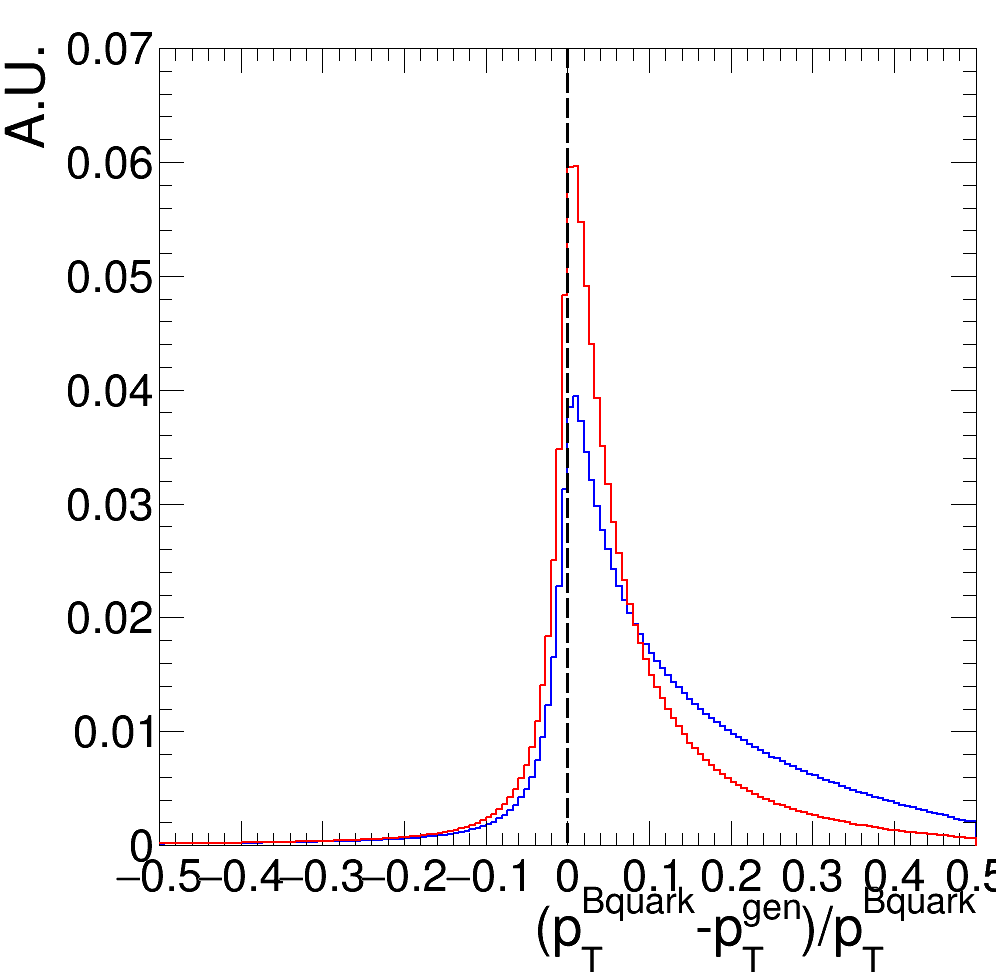
\includegraphics[width=0.35\textwidth]{b-reg/bQ_genPt_difference}\hfil
  \caption{Relative \PT difference of the b-quark and the
    corresponding gen-jet, obtained from $\HH\to\bbbb$ samples. Red
    histogram is for gen-jets containing neutrinos, blue is for jets
    without neutrinos.}
  \label{fig:b-reg-quark}
\end{figure*}


\begin{figure*}[thb]
  \centering
  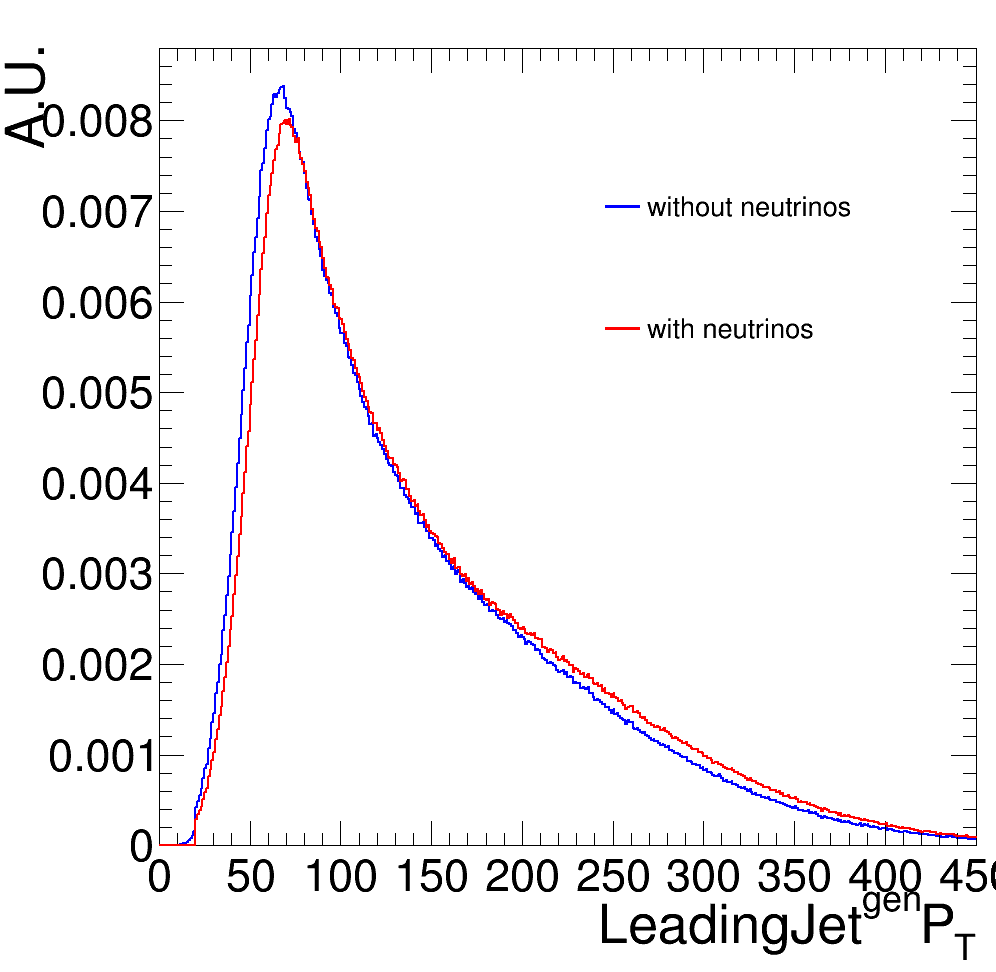
\includegraphics[width=0.45\textwidth]{b-reg/G_jet1_GenJetPt}\hfil
  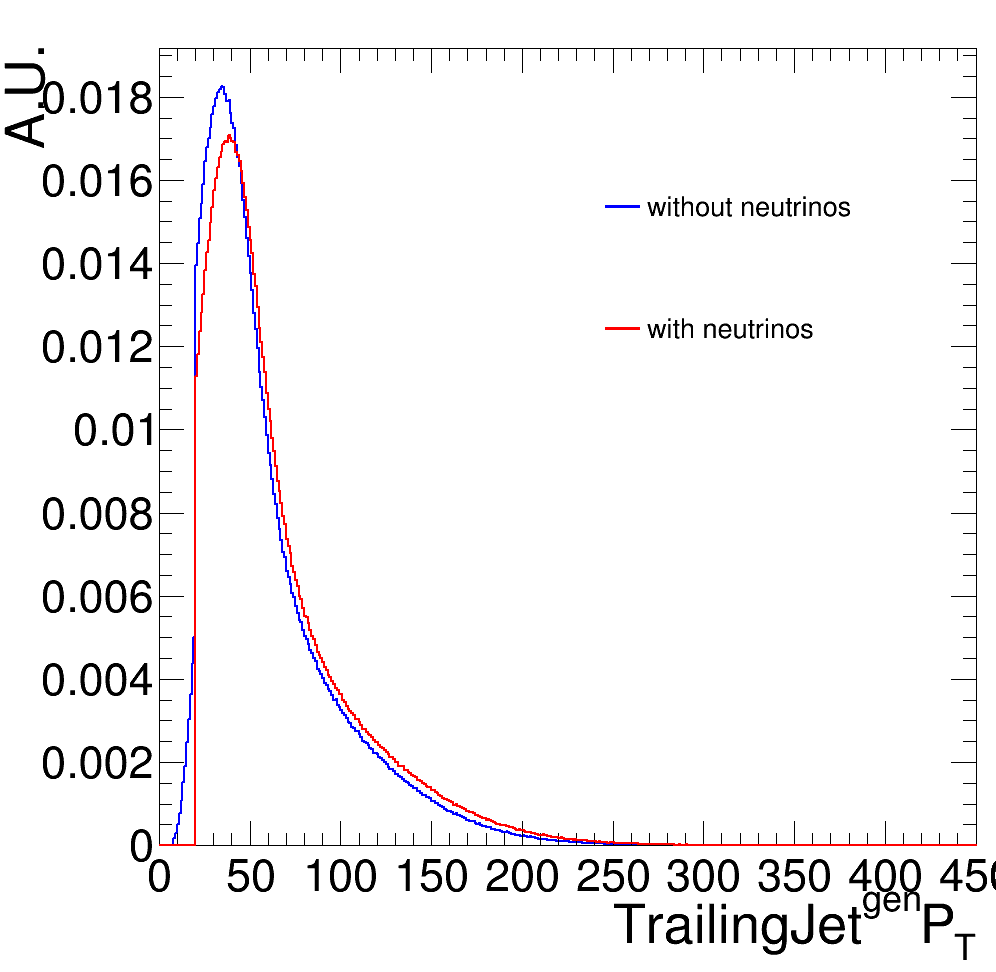
\includegraphics[width=0.45\textwidth]{b-reg/G_jet2_GenJetPt}\hfil\\
  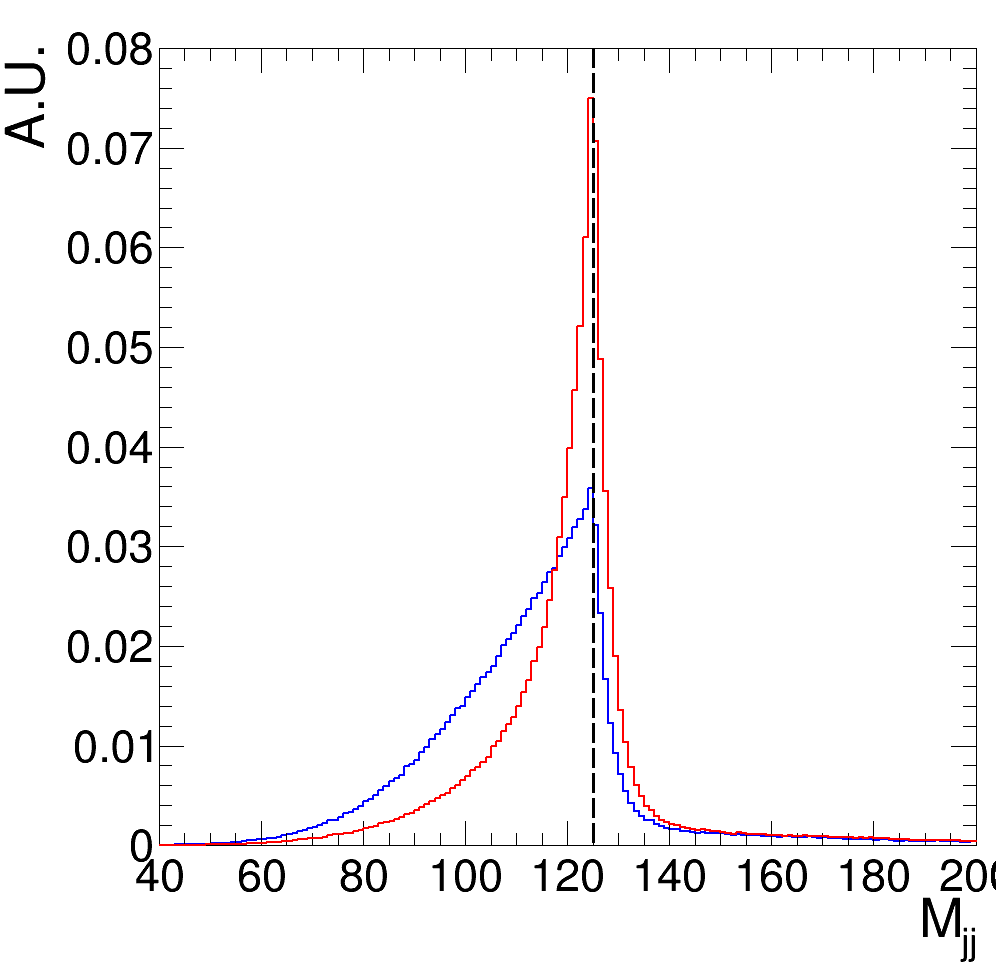
\includegraphics[width=0.45\textwidth]{b-reg/G_jjMass_Genjet}\hfil
  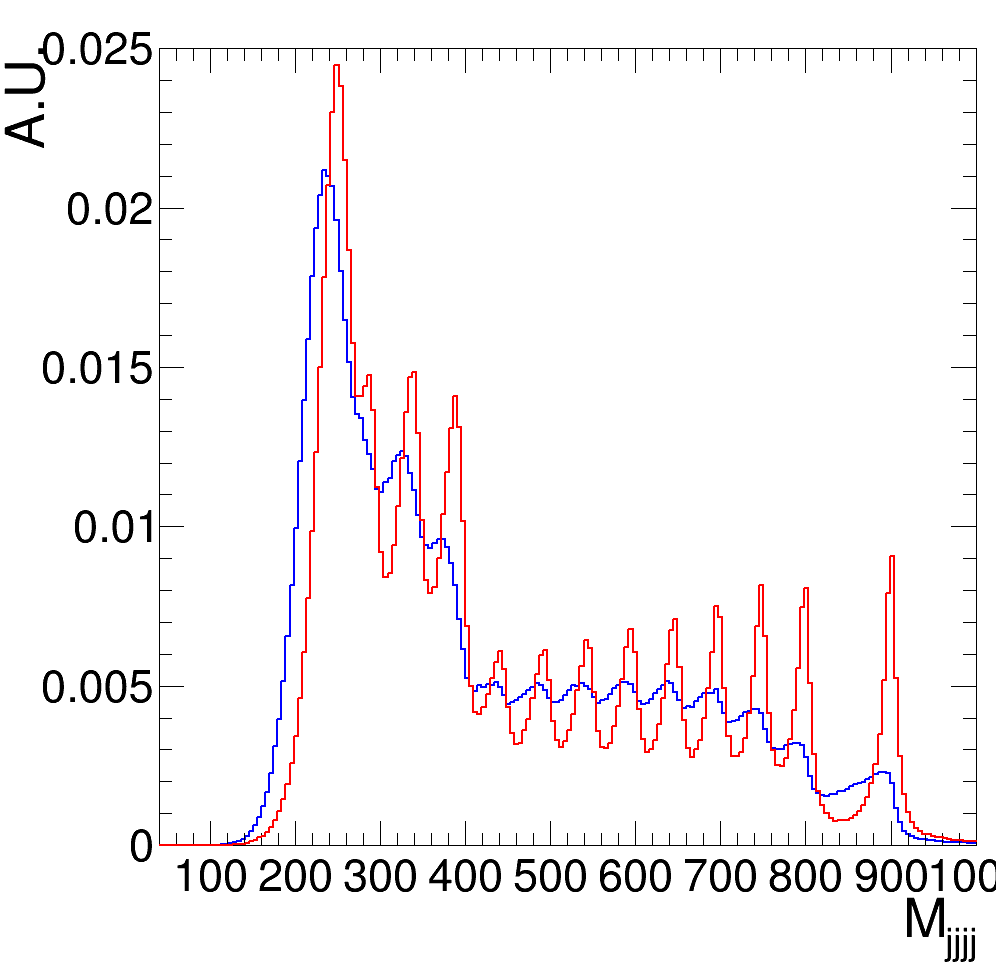
\includegraphics[width=0.45\textwidth]{b-reg/jjjjMass_jetGenJet}\hfil
  \caption{Leading and trailing jets \PT distributions (top), $m_{jj}$
    and $m_{jjjj}$ distributions, using jets in all samples with
    various $m_G$. Histogram obtained from $\HH\to\bbbb$ MC samples. Red
    histograms for gen-jets containing neutrinos, blue for jets
    without neutrinos.}
  \label{fig:b-reg-jet-neutrino}
\end{figure*}

\subsection{Training and performance}

For the training we select jets that satisfy the following criteria:
\begin{itemize}
\item $\PT > 20\GeV$, $|\eta| < 2.4$
\item Matched to the generated level jet within a cone $\DR<0.4$ (this matching is done as part of MiniAOD reconstruction)
\item Matched to a b-quark within a cone $\DR<0.4$
\end{itemize}


We perform three different trainings:
\begin{itemize}
\item Using only the 16 variables as in $\Hbb$ training, denoted as
  \textbf{16var} on the figures below.
\item Using the 16 variables plus \MET and $\Delta\Phi(Jet,
  \MET)$. This training is denoted as \textbf{16plus2} on the figures.
\item Using the 16 plus 2 variables as above but in addition, for each
  pair of jets from the Higgs boson, the training is performed
  separately for the leading and trailing jets. That is, two XML
  weight files are derived, one for the leading and one for the
  trailing jet in the event.  This training is denoted as
  \textbf{16plus2 js} on the figures.
\item Using all 19 variables listed in Table~\ref{tab:reg-vars}, and
  separating the training for leading and trailing jets as above. This
  training is denoted as \textbf{16plus3 js} on the figures.
\end{itemize}
We compare those trainings with the one done by $\Hbb$ analysis, which
is denoted as \textbf{Hbb} on the figures.


After the training is done, its performance is checked in signal
samples, $X\to\HH\to\ggbb$, at all mass points of $m_X$.  The
$\PT^{reco}$ of the reconstructed jet can be compared to the target
$\PT^{gen}$ of the generated jet. An example of such distributions is
shown in Fig.~\ref{fig:b-reg-pt-res} for the leading and trailing
jets. From distributions such as in Fig.~\ref{fig:b-reg-pt-res} we
obtain the mean value for the \textbf{scale} and sigma ($\sigma$) for
the \textbf{resolution}. For the sigma we use the so-called
``effective sigma'', which is the minimum width of the histogram that
contains 68\% of events. The scale and resolution of the leading and
trailing jets versus their \PT are shown in
Fig.~\ref{fig:b-reg-jet-res}. From this figure we can conclude that
adding MET variables into the taring improves significantly the
resolution.  As expected the \textbf{16plus3 js} training gives best
per-jet resolution across the whole \PT range. The training training,
with \textbf{16} variables gives similar result to the \textbf{Hbb}
training.

\begin{figure*}[bth]
  \centering
  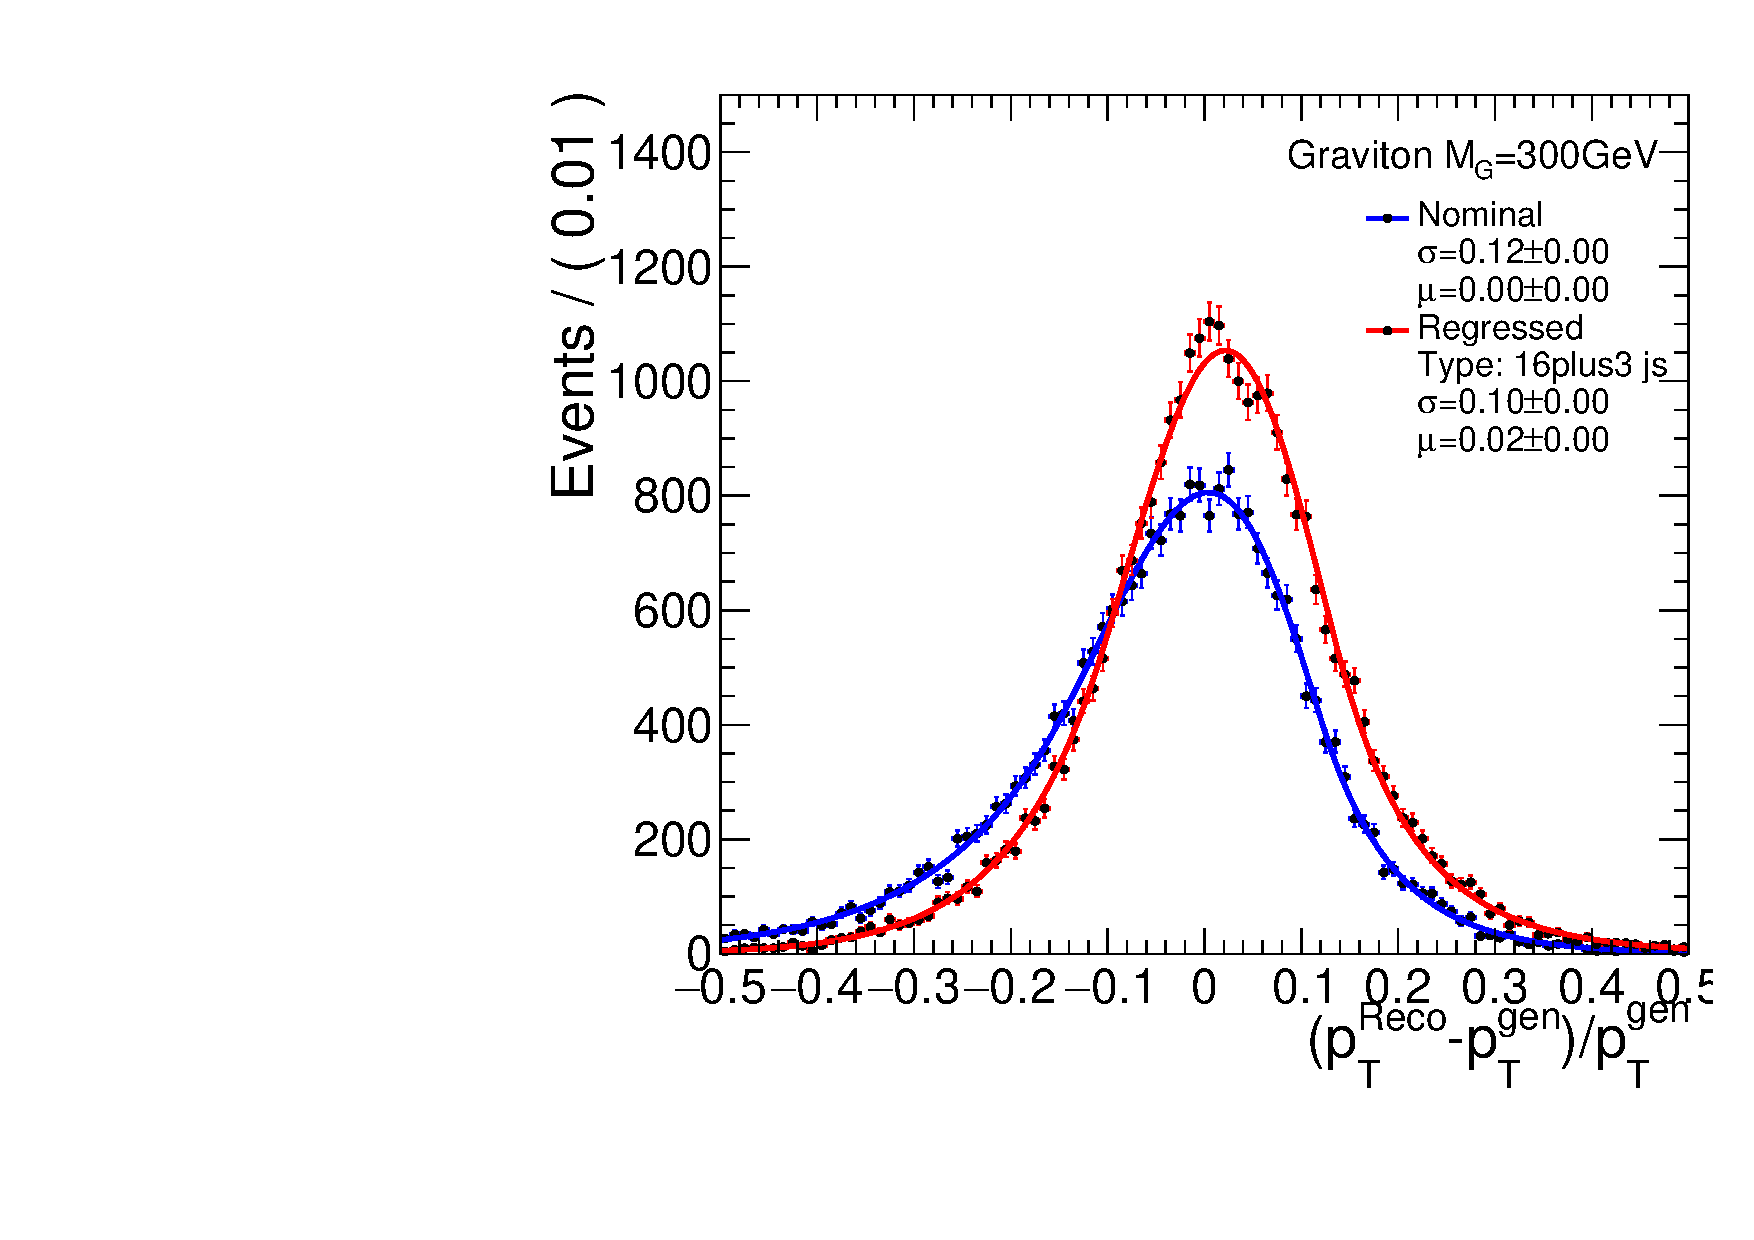
\includegraphics[width=0.45\textwidth]{b-reg/G_jet1_PtResolution}\hfil
  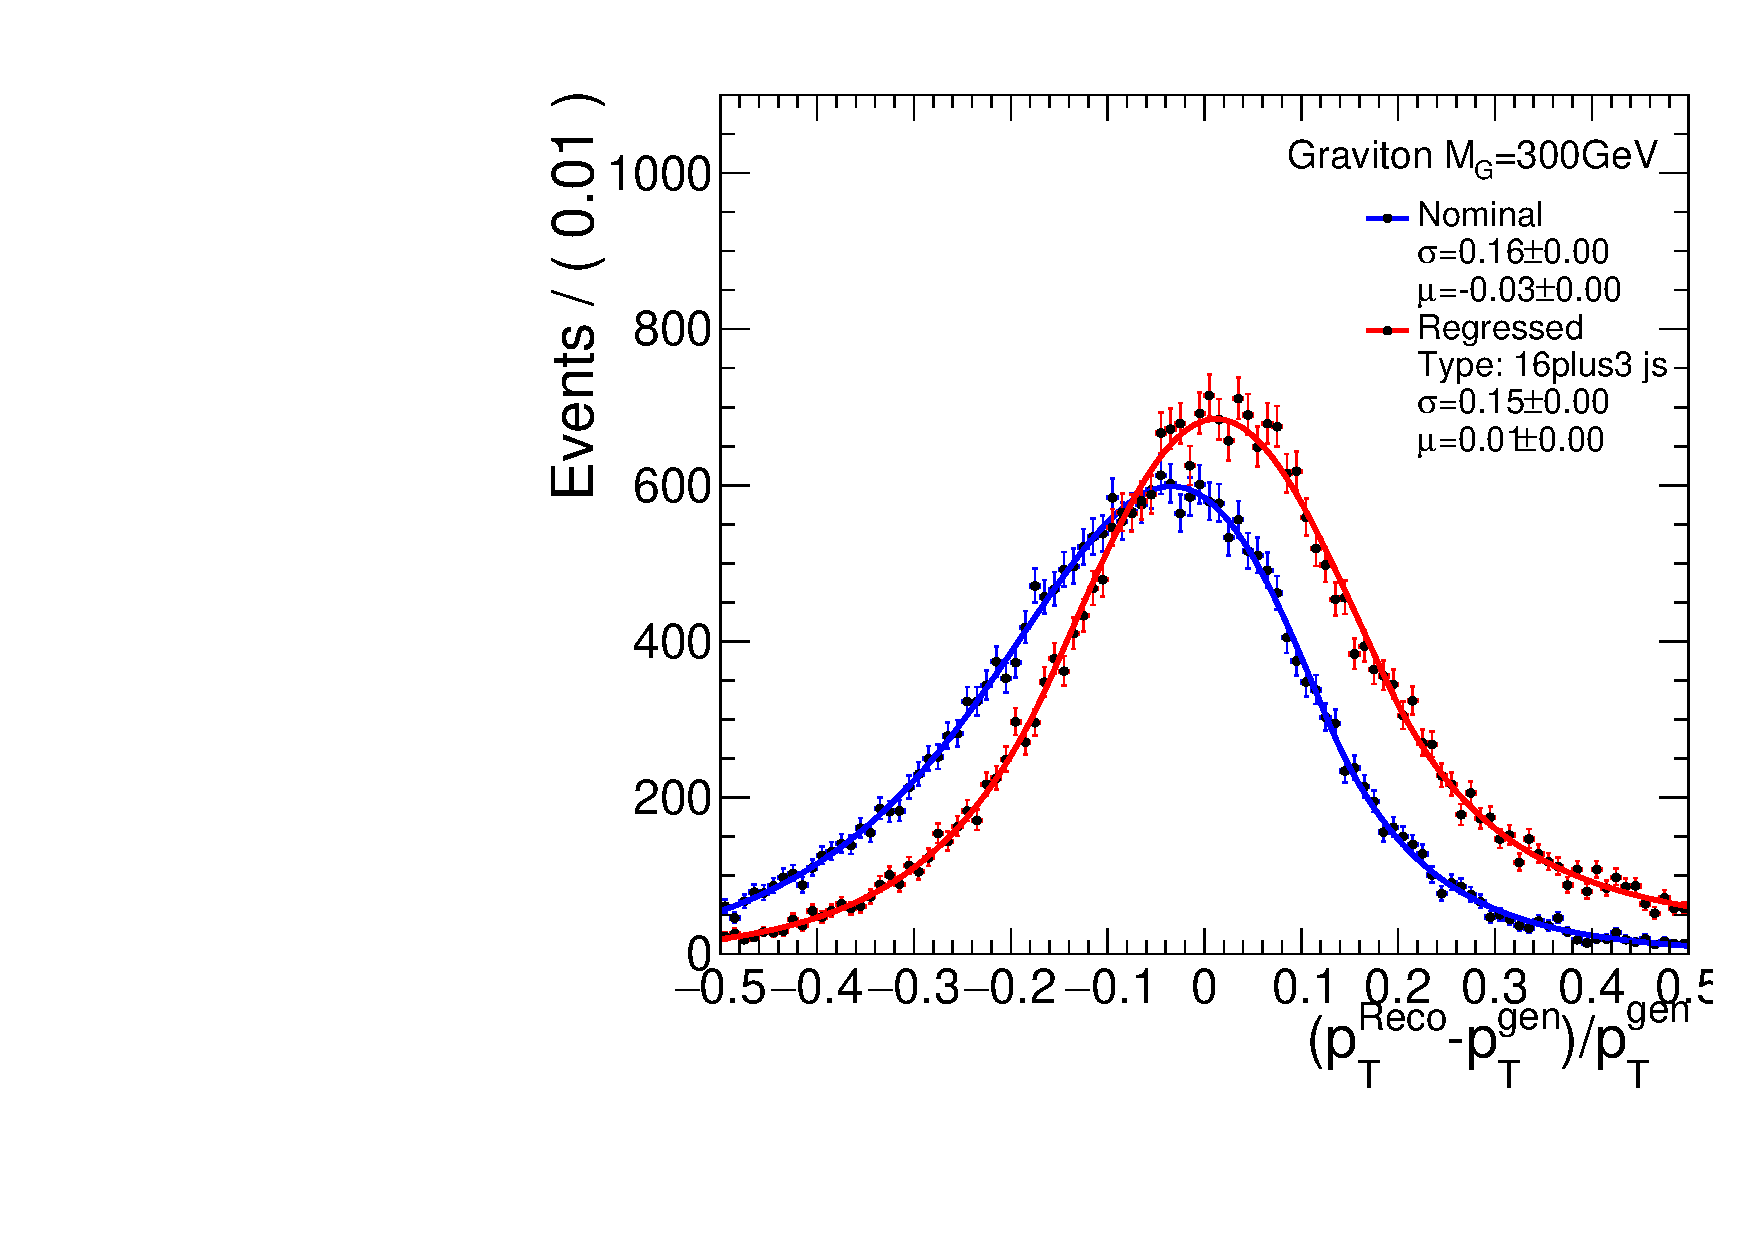
\includegraphics[width=0.45\textwidth]{b-reg/G_jet2_PtResolution}\hfil
  \caption{Relative \PT difference of the reconstructed and generated
    level jets after regression (red histograms) and without
    the regression (blue histograms).}
  \label{fig:b-reg-pt-res}
\end{figure*}

\begin{figure*}[bth]
  \centering
  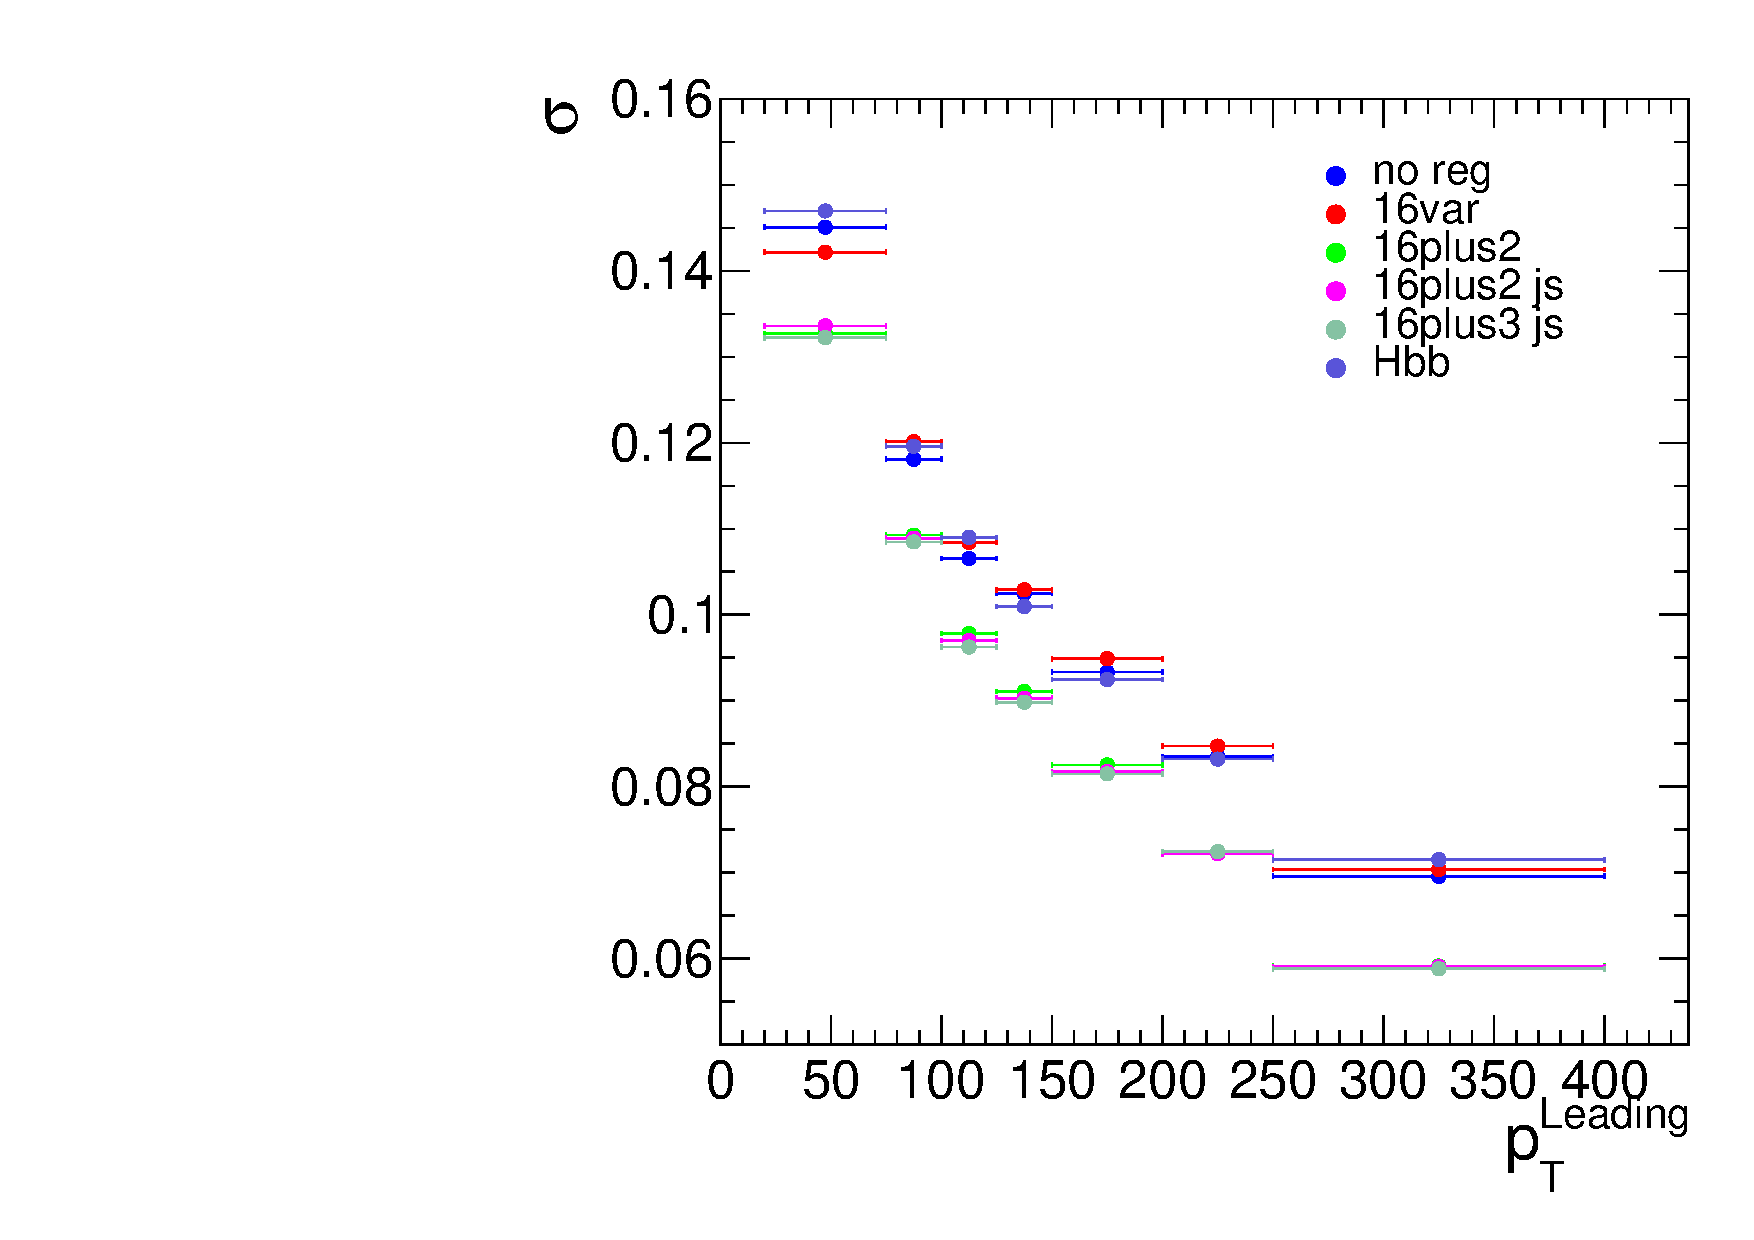
\includegraphics[width=0.45\textwidth]{b-reg/sigma_pT_jet1}\hfil
  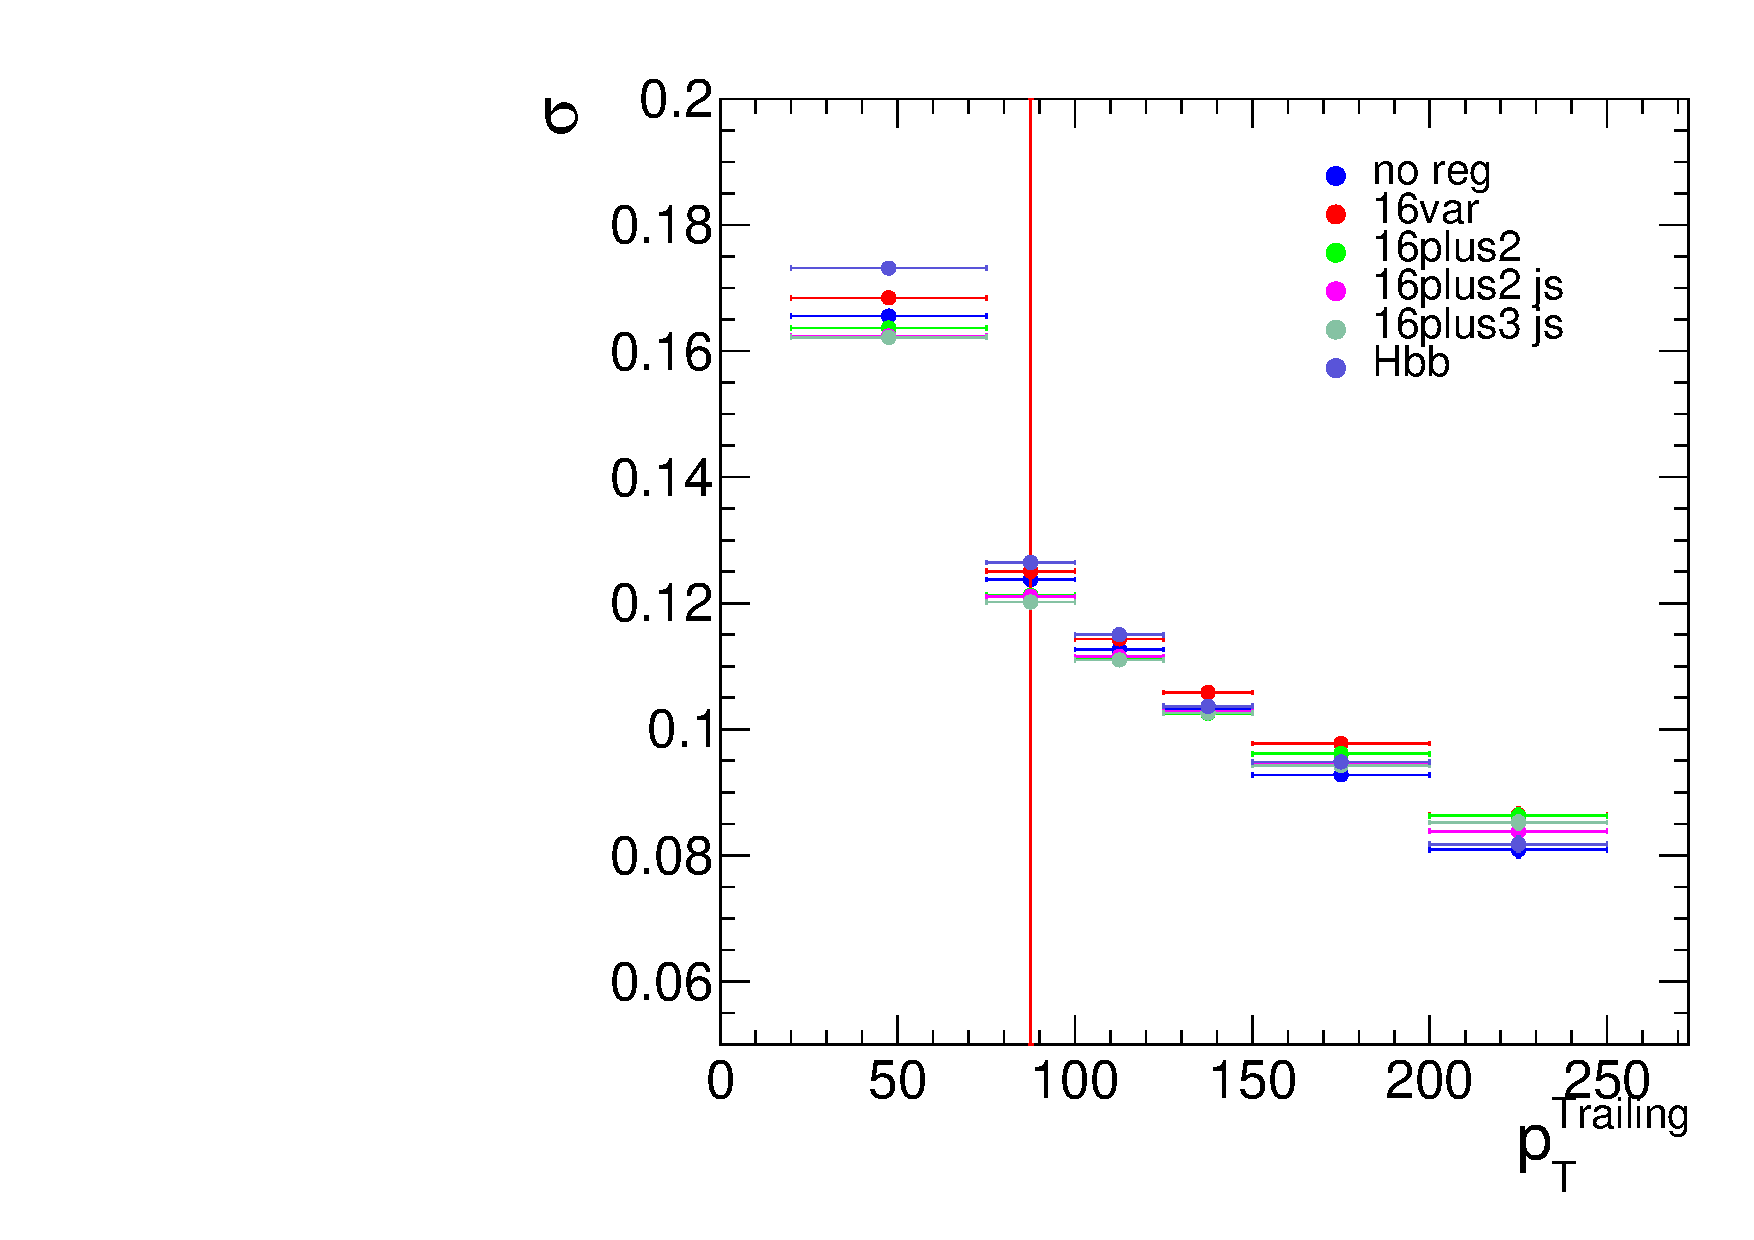
\includegraphics[width=0.45\textwidth]{b-reg/sigma_pT_jet2}\hfil\\
  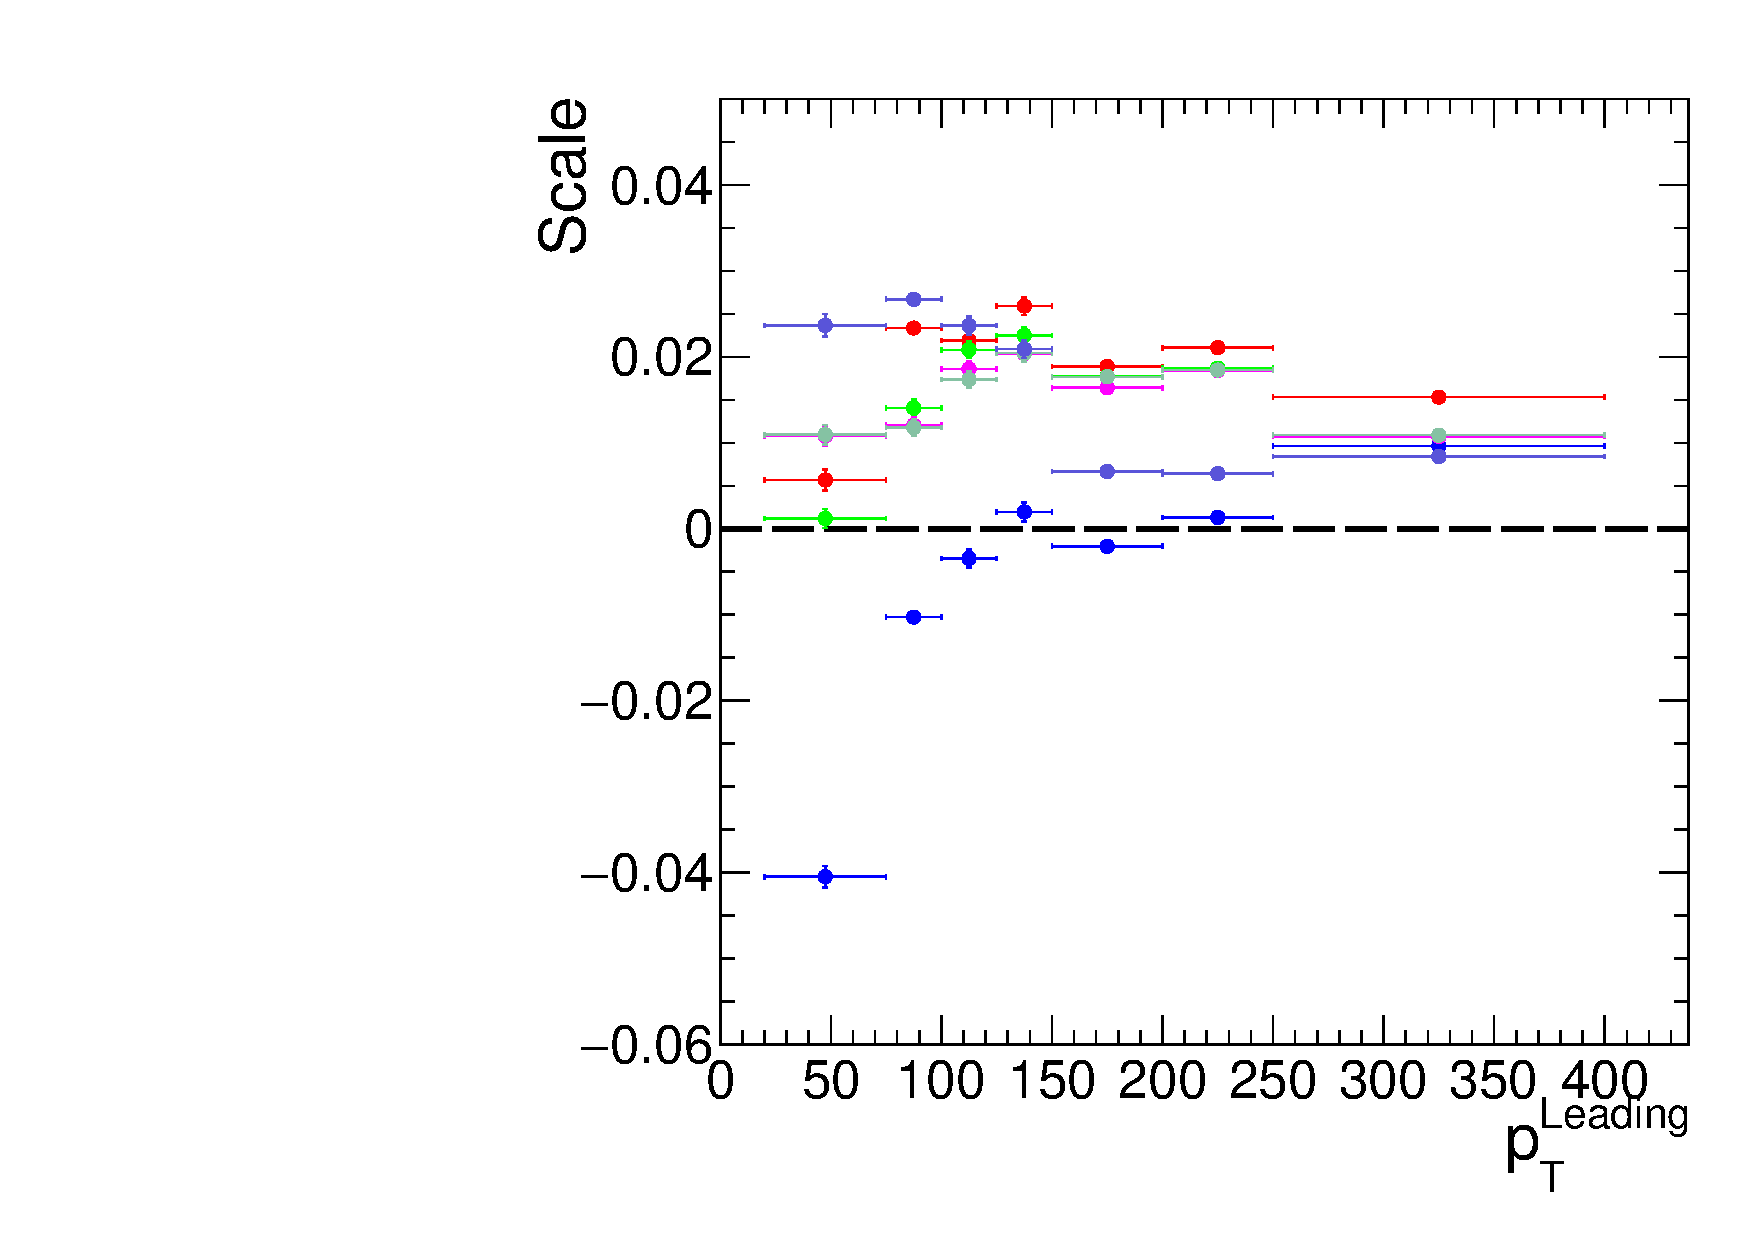
\includegraphics[width=0.45\textwidth]{b-reg/scale_pT_jet1}\hfil
  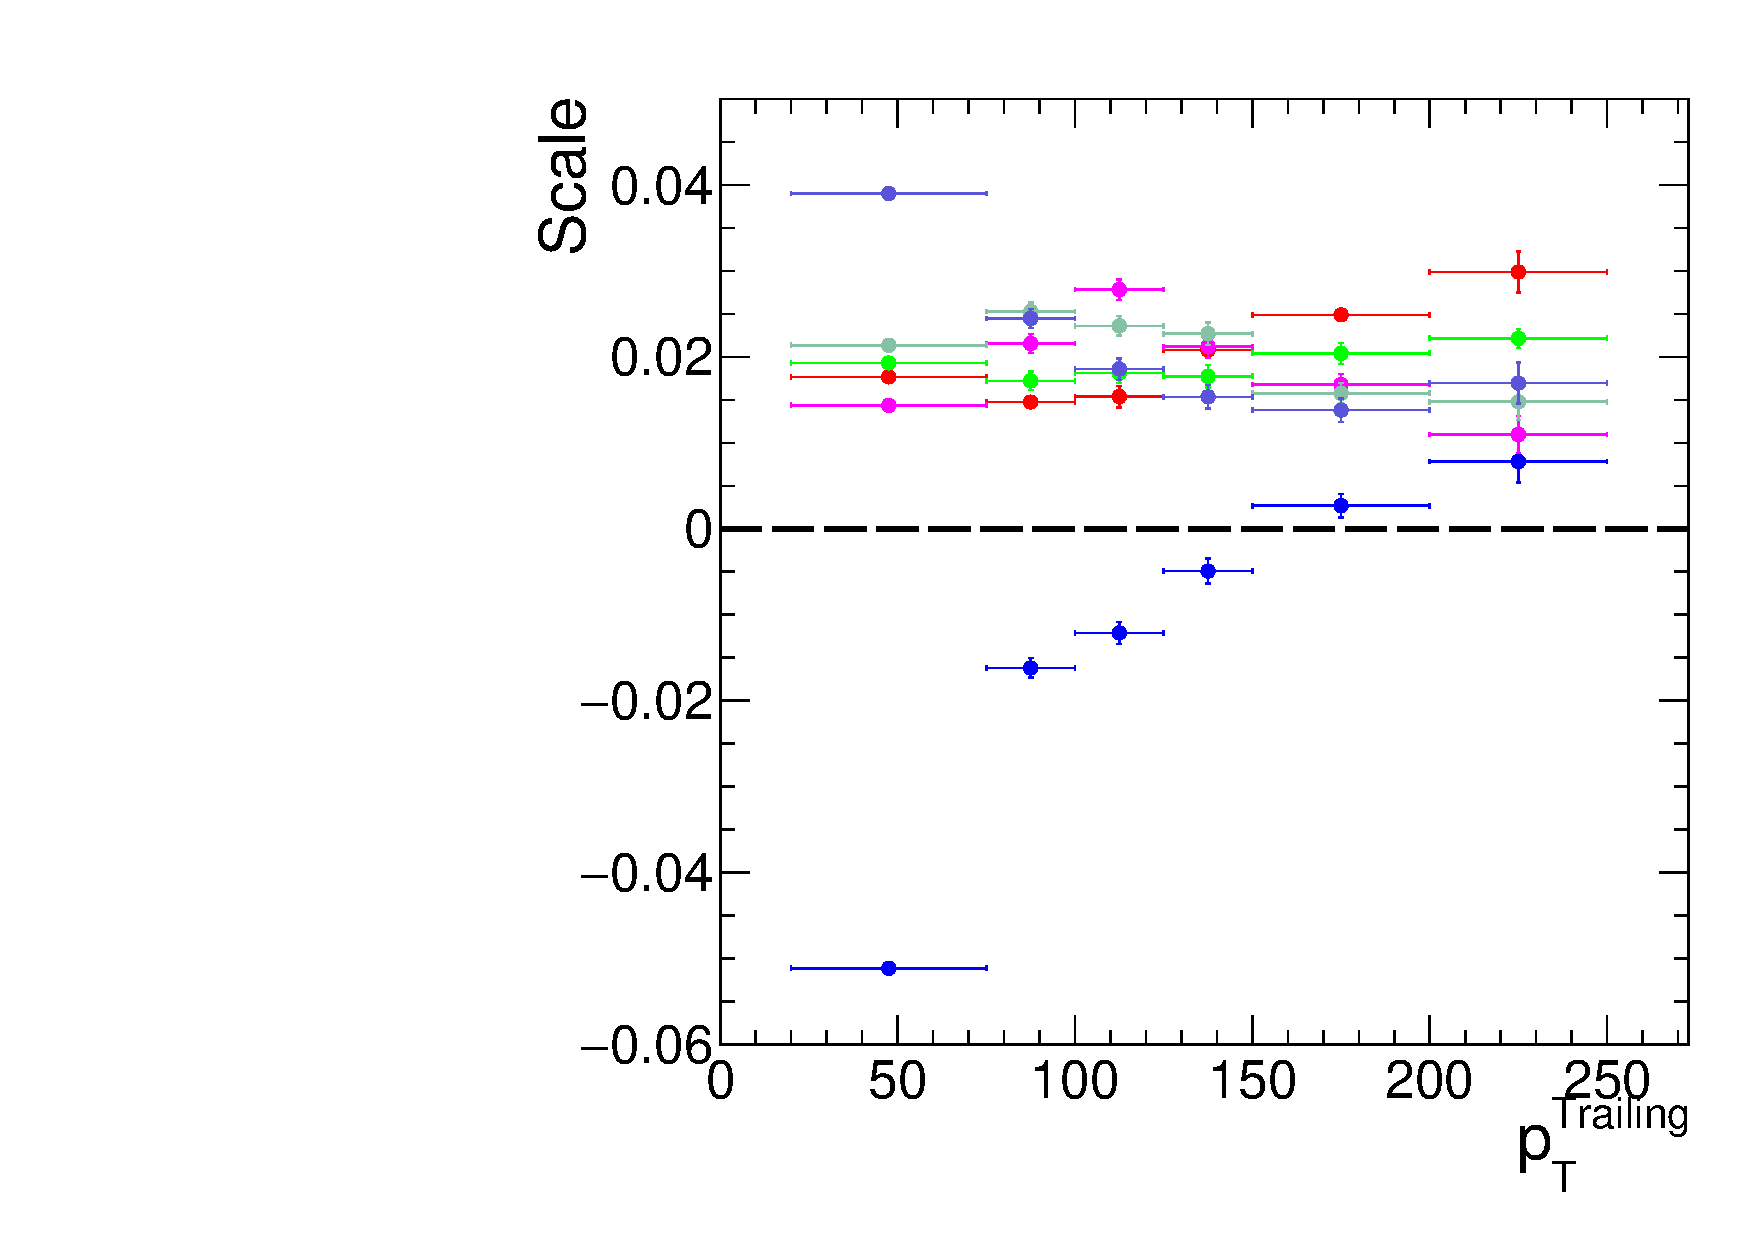
\includegraphics[width=0.45\textwidth]{b-reg/scale_pT_jet2}\hfil\\
  \caption{The resolution of the jet \PT (top) and the scale (bottom),
    for leading (left) and trailing (right) jets from the signal
    sample $G\to\HH\to\ggbb$.}
  \label{fig:b-reg-jet-res}
\end{figure*}

\clearpage
\subsection{Mass resolution}
The purpose of the regression is to improve the Higgs boson mass
resolution from the $\Hbb$ decay in $X\to\HH\to\ggbb$ signal. Before
we show the effect of the regression on the Higgs boson candidate
mass, we must note that the $m_{jj}$ distributions are highly
asymmetric. For that reason we choose to fit those distributions with
Bukin functions, examples of which are shown in
Figs.~\ref{fig:b-reg-mH-fit-reco}.  In the
Fig.~\ref{fig:b-reg-mH-fit-reco} the distribution of the reconstructed
mass is shown after \textbf{16plus3 js} regression training, for $m_G
= 300\GeV$ and SM samples.  The fits in those cases look good.
However, when we try to perform this fit on the mass distribution
obtained with the gen-jets, as shown in
Fig.~\ref{fig:b-reg-mH-fit-gen}, the Bukin function does not give us a
good fit. We decided to use the fit of Gaussian to the core of the
distribution for the gen-level mass, as also shown in that figure.

\begin{figure*}[b]
  \centering
  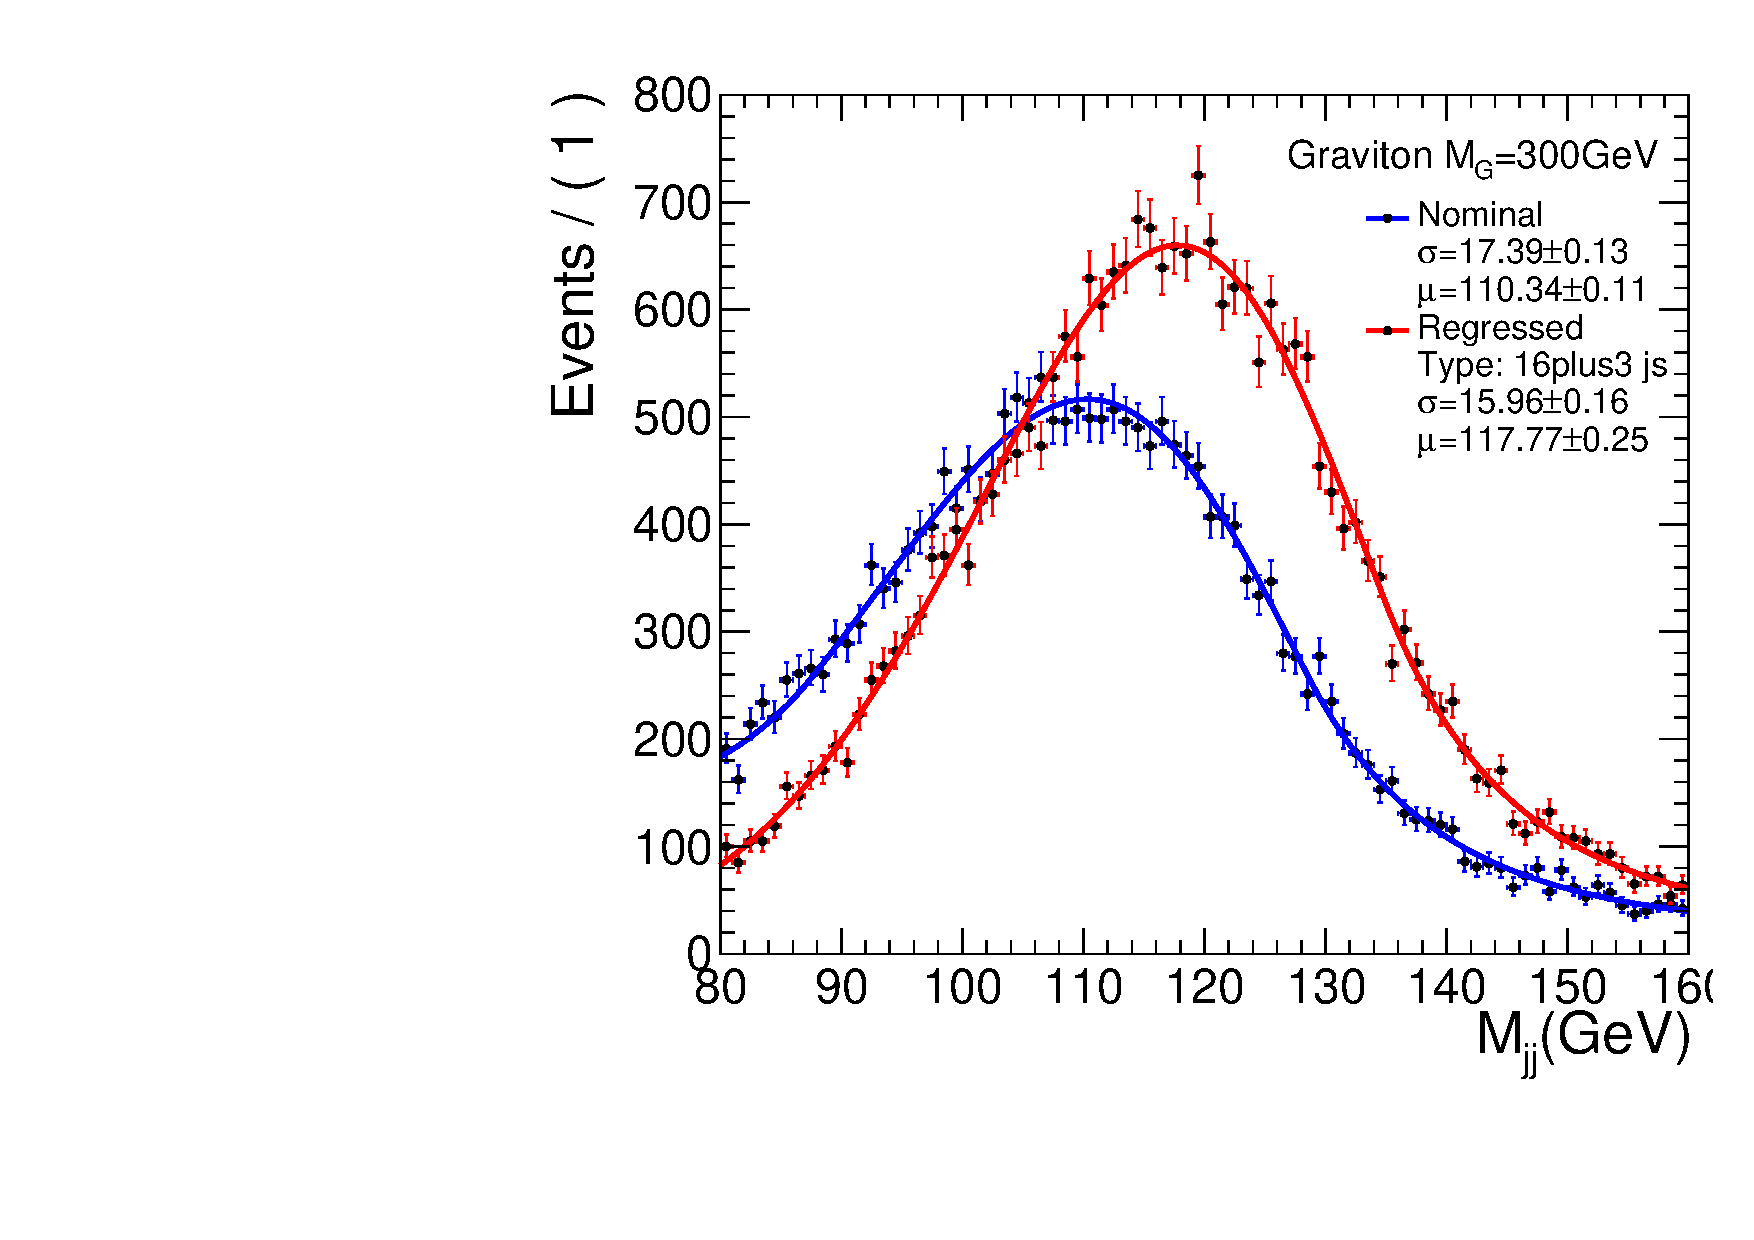
\includegraphics[width=0.45\textwidth]{b-reg/Bukin_mjj_G300}\hfil
  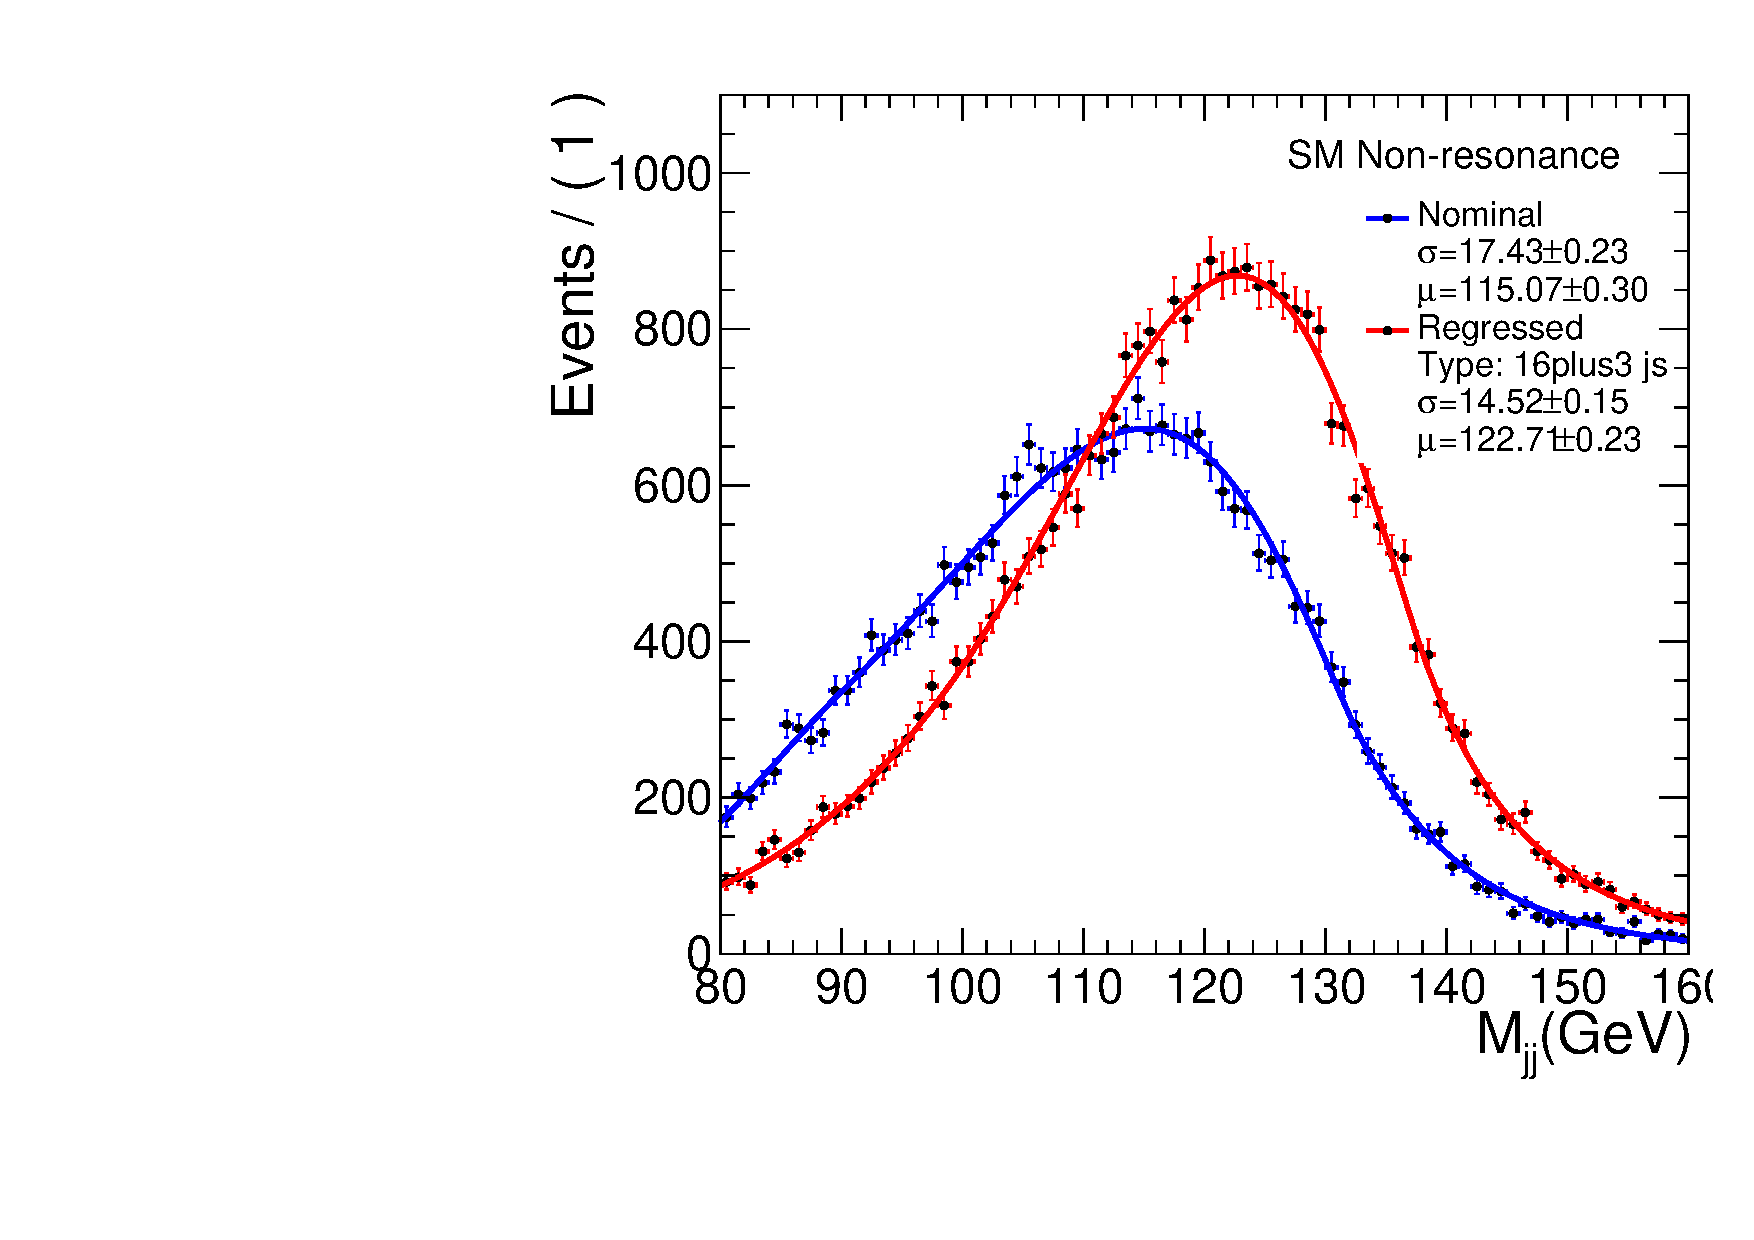
\includegraphics[width=0.45\textwidth]{b-reg/Bukin_mjj_SM}\hfil
  \caption{$M_{jj}$ distributions from the reco-jets before and after
    the \textbf{16plus3 js} regression for $m_G=300\GeV$ signal sample
    (left) and SM sample (right).}
  \label{fig:b-reg-mH-fit-reco}
\end{figure*}

\begin{figure*}[thb]
  \centering
  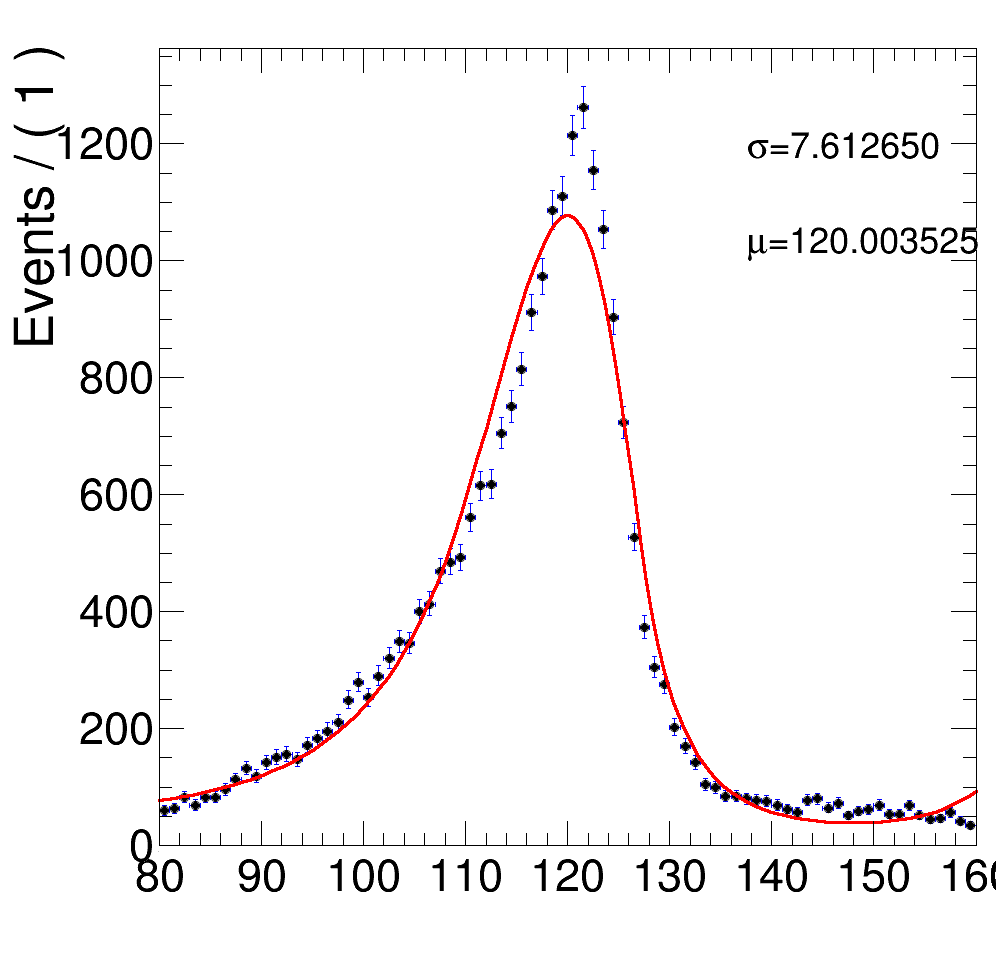
\includegraphics[width=0.45\textwidth]{b-reg/Bukin_G76_mass_MassR_jetgenJet_eff_m300}\hfil
  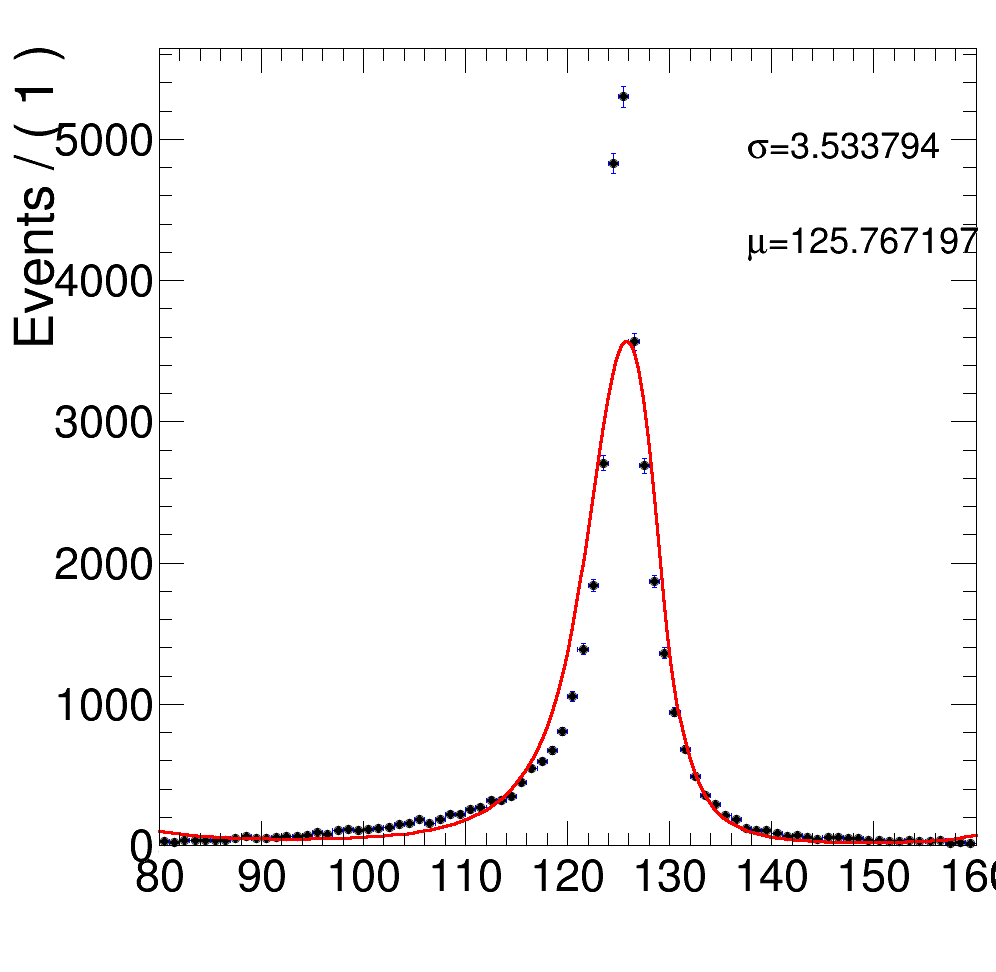
\includegraphics[width=0.45\textwidth]{b-reg/Bukin_G76_mass_MassR_jetgenJet_eff_m900}\hfil\\
  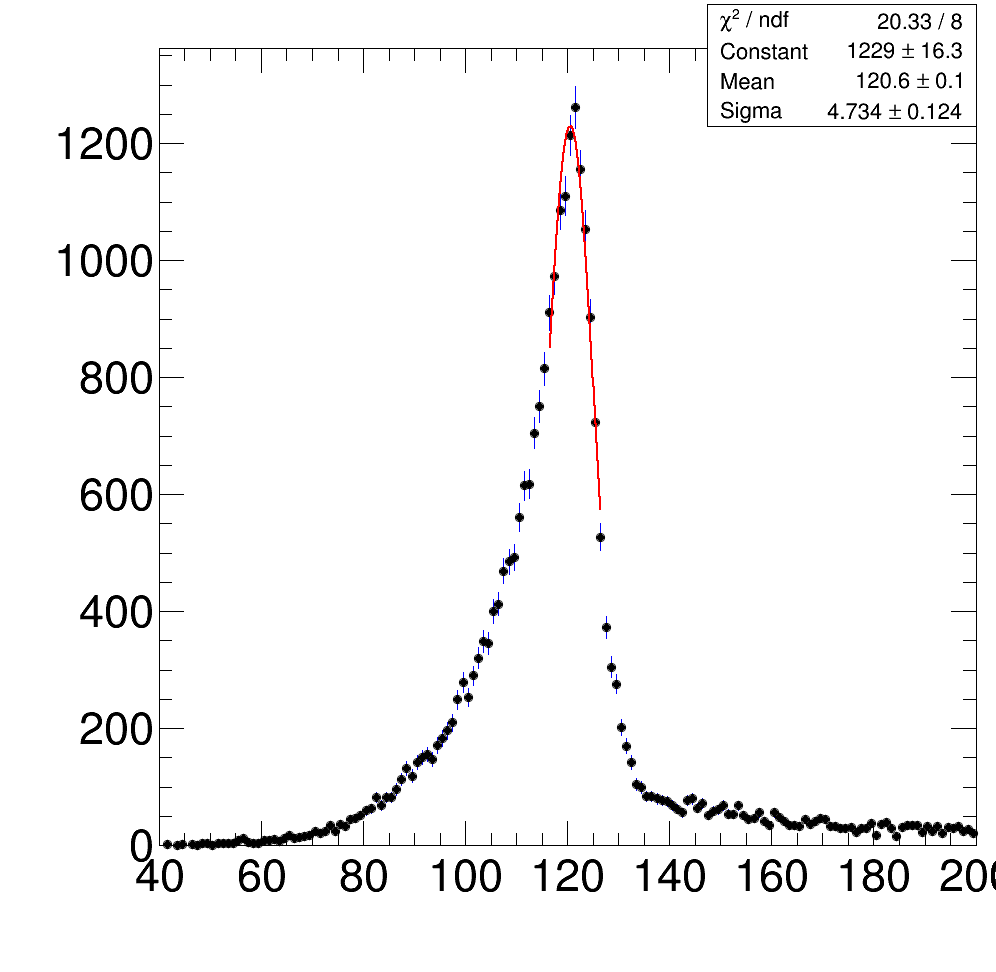
\includegraphics[width=0.45\textwidth]{b-reg/Gaussian_G76_mass_MassR_jetgenJet_eff_m300}\hfil
  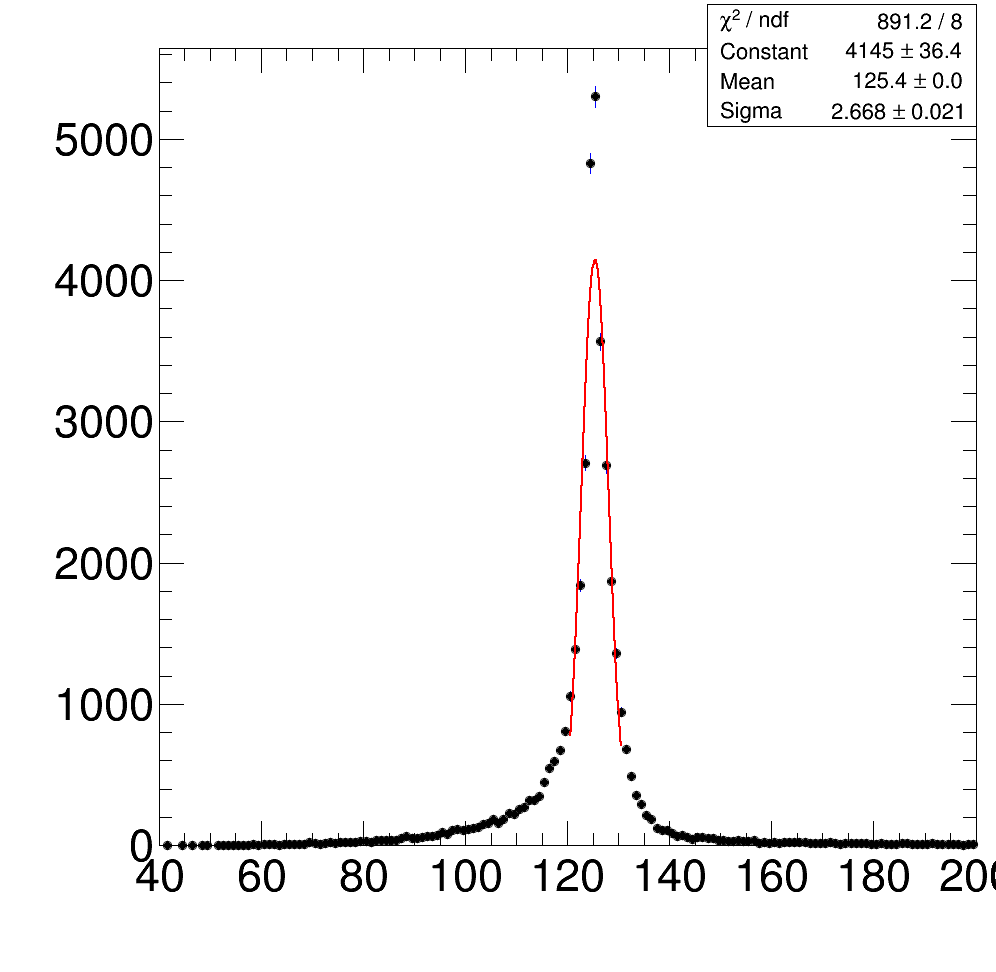
\includegraphics[width=0.45\textwidth]{b-reg/Gaussian_G76_mass_MassR_jetgenJet_eff_m900}\hfil
  \caption{Bukin function (top) and Gaussian (bottom) fits of the
    $m_{jj}$ distributions, obtained from gen-jets. Left plots are for
    $m_G=300\GeV$ sample, right is $m_G=900\GeV$}
  \label{fig:b-reg-mH-fit-gen}
\end{figure*}



Finally, after the fitting to the corresponding function is done, we
obtain the mean and the width parameters of the fit.  The width (in
\GeV) and mean are shown on Fig.~\ref{fig:b-reg-mH-res} versus the
mass of the Graviton particle.  From this figure we arrive at the same
conclusion as for single-jet plots of Fig.~\ref{fig:b-reg-jet-res}:
the \textbf{16plus4 js} training gives the best mass resolution. The
training with \textbf{16} variables give similar results to the
\textbf{Hbb} training.  In all trainings the scale does not match
the nominal value of the Higgs boson mass. This is expected because
the jets (both at reco and gen levels) do not contain the whole energy
of the Higgs boson decay.


\begin{figure*}[thb]
  \centering
  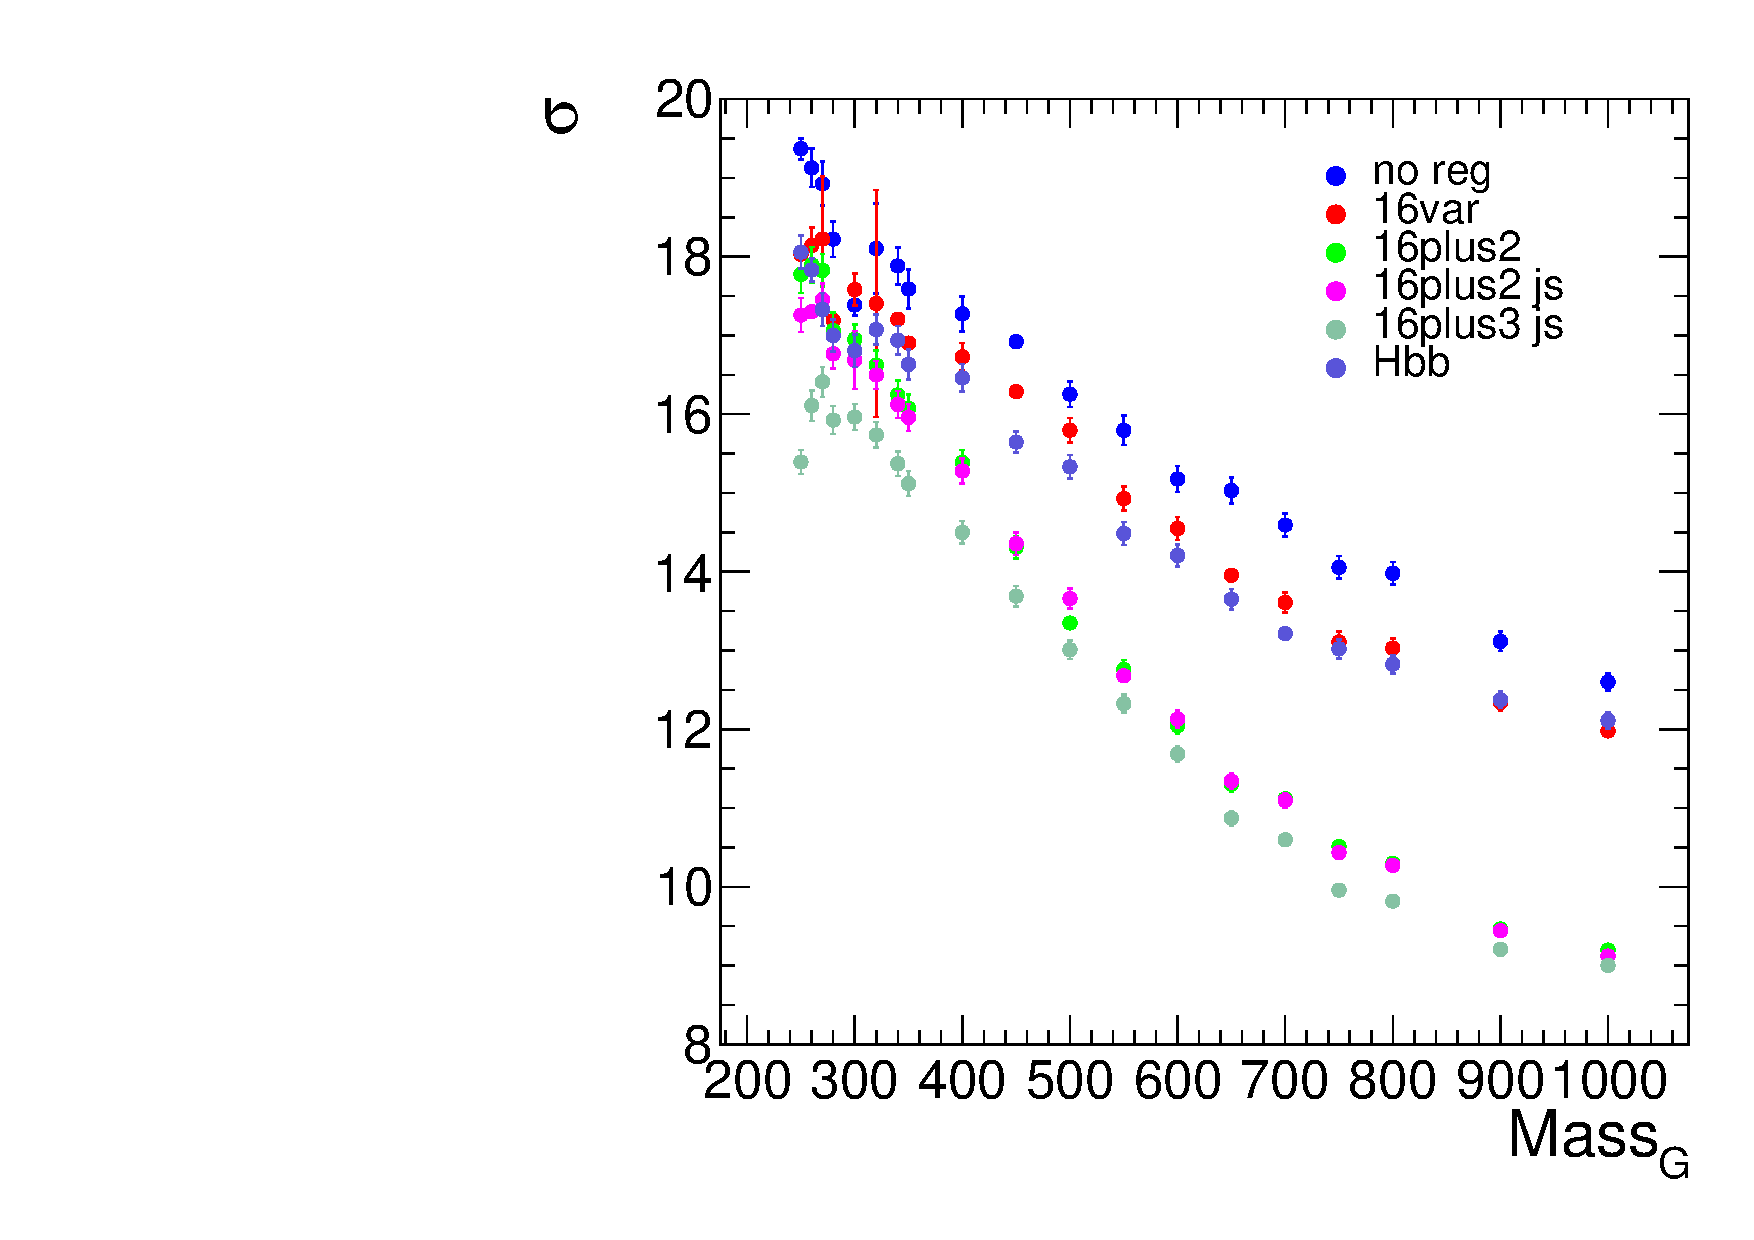
\includegraphics[width=0.45\textwidth]{b-reg/sigma_mass_mjj}\hfil
  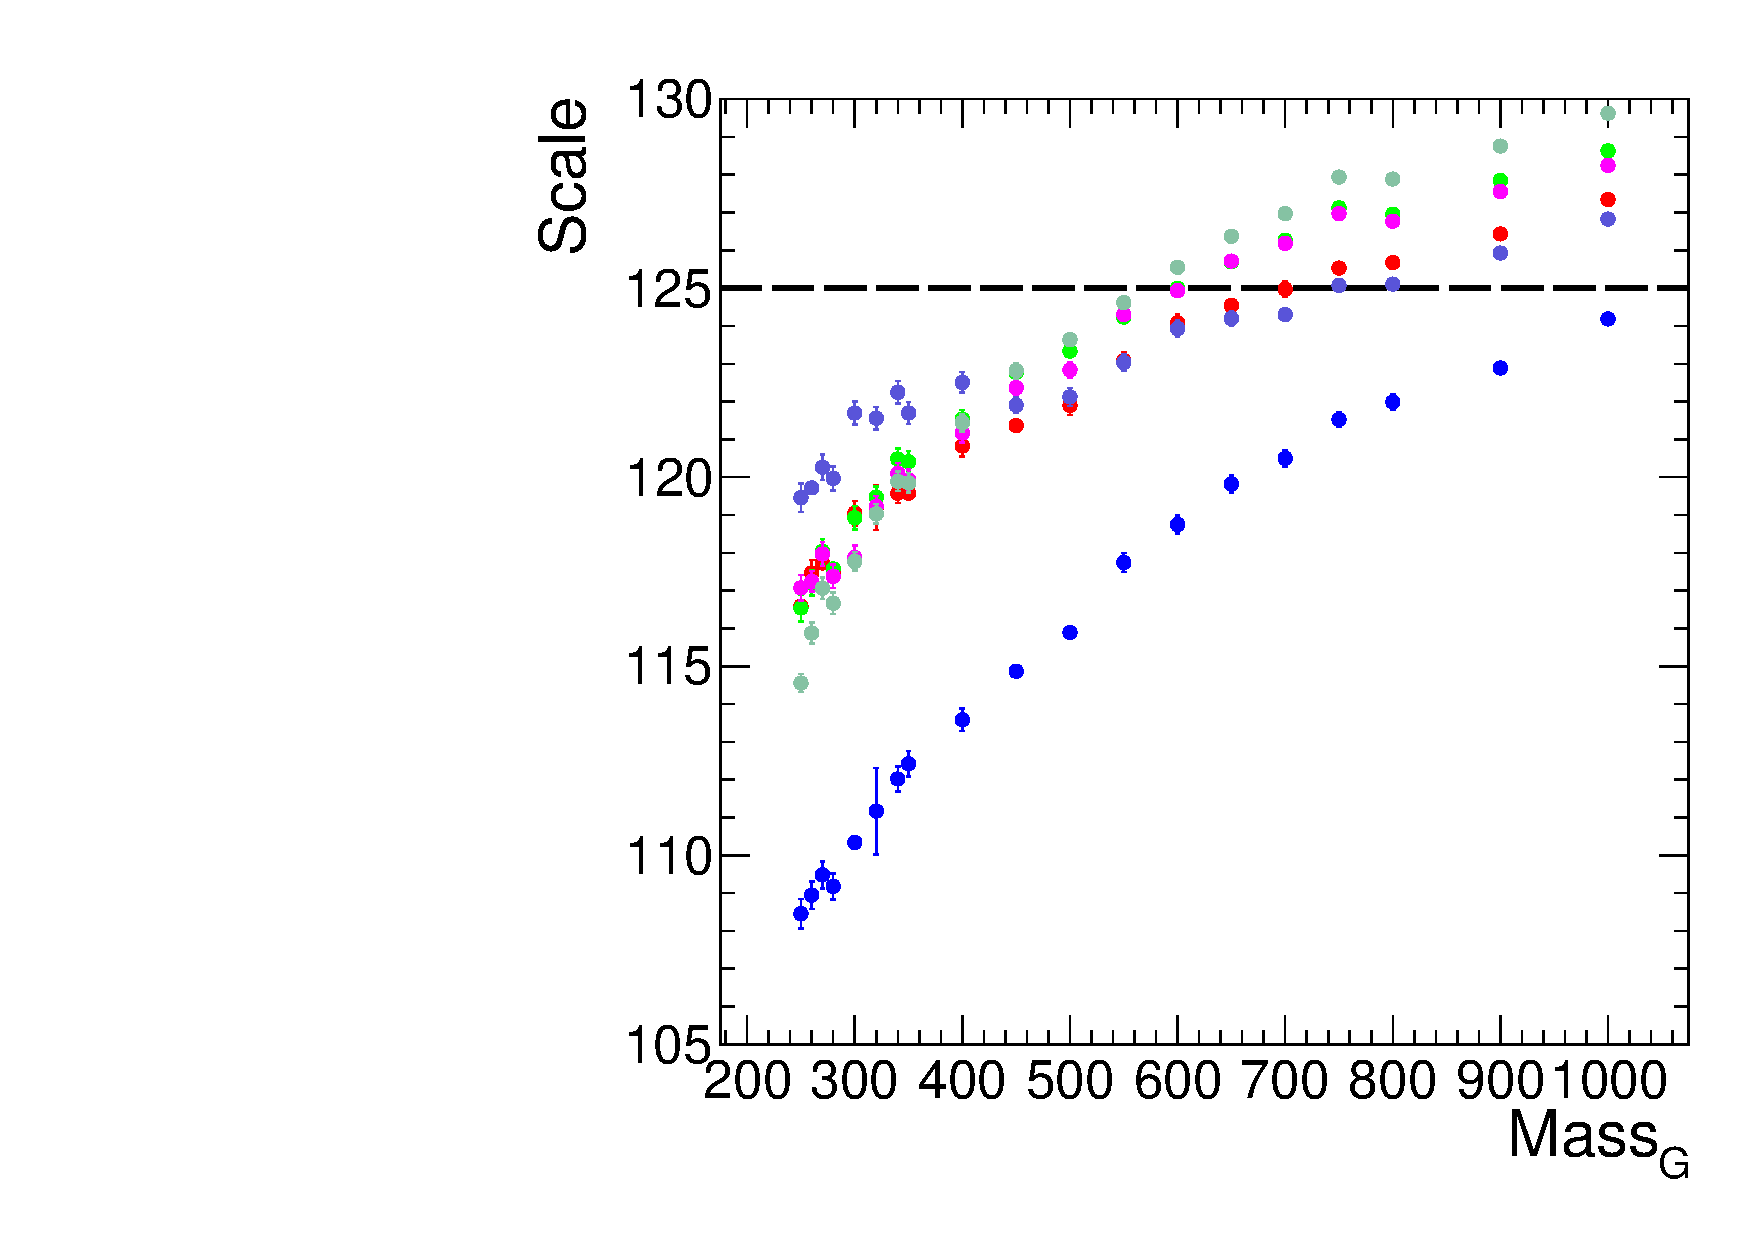
\includegraphics[width=0.45\textwidth]{b-reg/scale_mass_mjj}\hfil
  \caption{Performance plot comparing different regression trainings.}
  \label{fig:b-reg-mH-res}
\end{figure*}


\clearpage
\subsection{Validation in data}

In order to validate the developed regression in data we select events
with $\Z\to\ell\ell$ decay which also contain two b-tagged jets. It is
assumed that a di-jet must be recoiled against $\Z$ boson, and
therefore the $\PT(jj)$ must balance the $\PT(\ell\ell)$.  This check
was done both in muon and electron channels of \Z boson decay,
analyzing DoubleMuon and DoubleElectron datasets correspondingly,
using 2016-BCD data. In the muon channel the events were selected with
an OR of \verb|HLT_Mu17_TrkIsoVVL_Mu8_TrkIsoVVL_DZ| and
\verb|HLT_Mu17_TrkIsoVVL_TkMu8_TrkIsoVVL_DZ| triggers and the
reconstructed muons must pass Tight muon ID and Loose PF
isolation. While in the electron channel the
\verb|HLT_Ele23_Ele12_CaloIdL_TrackIdL_IsoVL_DZ| trigger was used and
the electrons required to pass MVA ID WP90 selection.  Further event
selection requirements in both channels are: $\PT(\ell_1) > 25\GeV$,
$\PT(\ell_2) > 15\GeV$, $\PT(\ell\ell) > 50\GeV$,
$75<m_{\ell\ell}<105\GeV$, $\Delta R^{min}_{\ell, jet} > 0.4$. The two
jets in the event must pass Loose PF ID selection, tagged as b-jets
with CSVv2 Loose WP, and have $\PT>20\GeV$, $|\eta|<2.4$.


\begin{figure*}[thb]
  \centering
  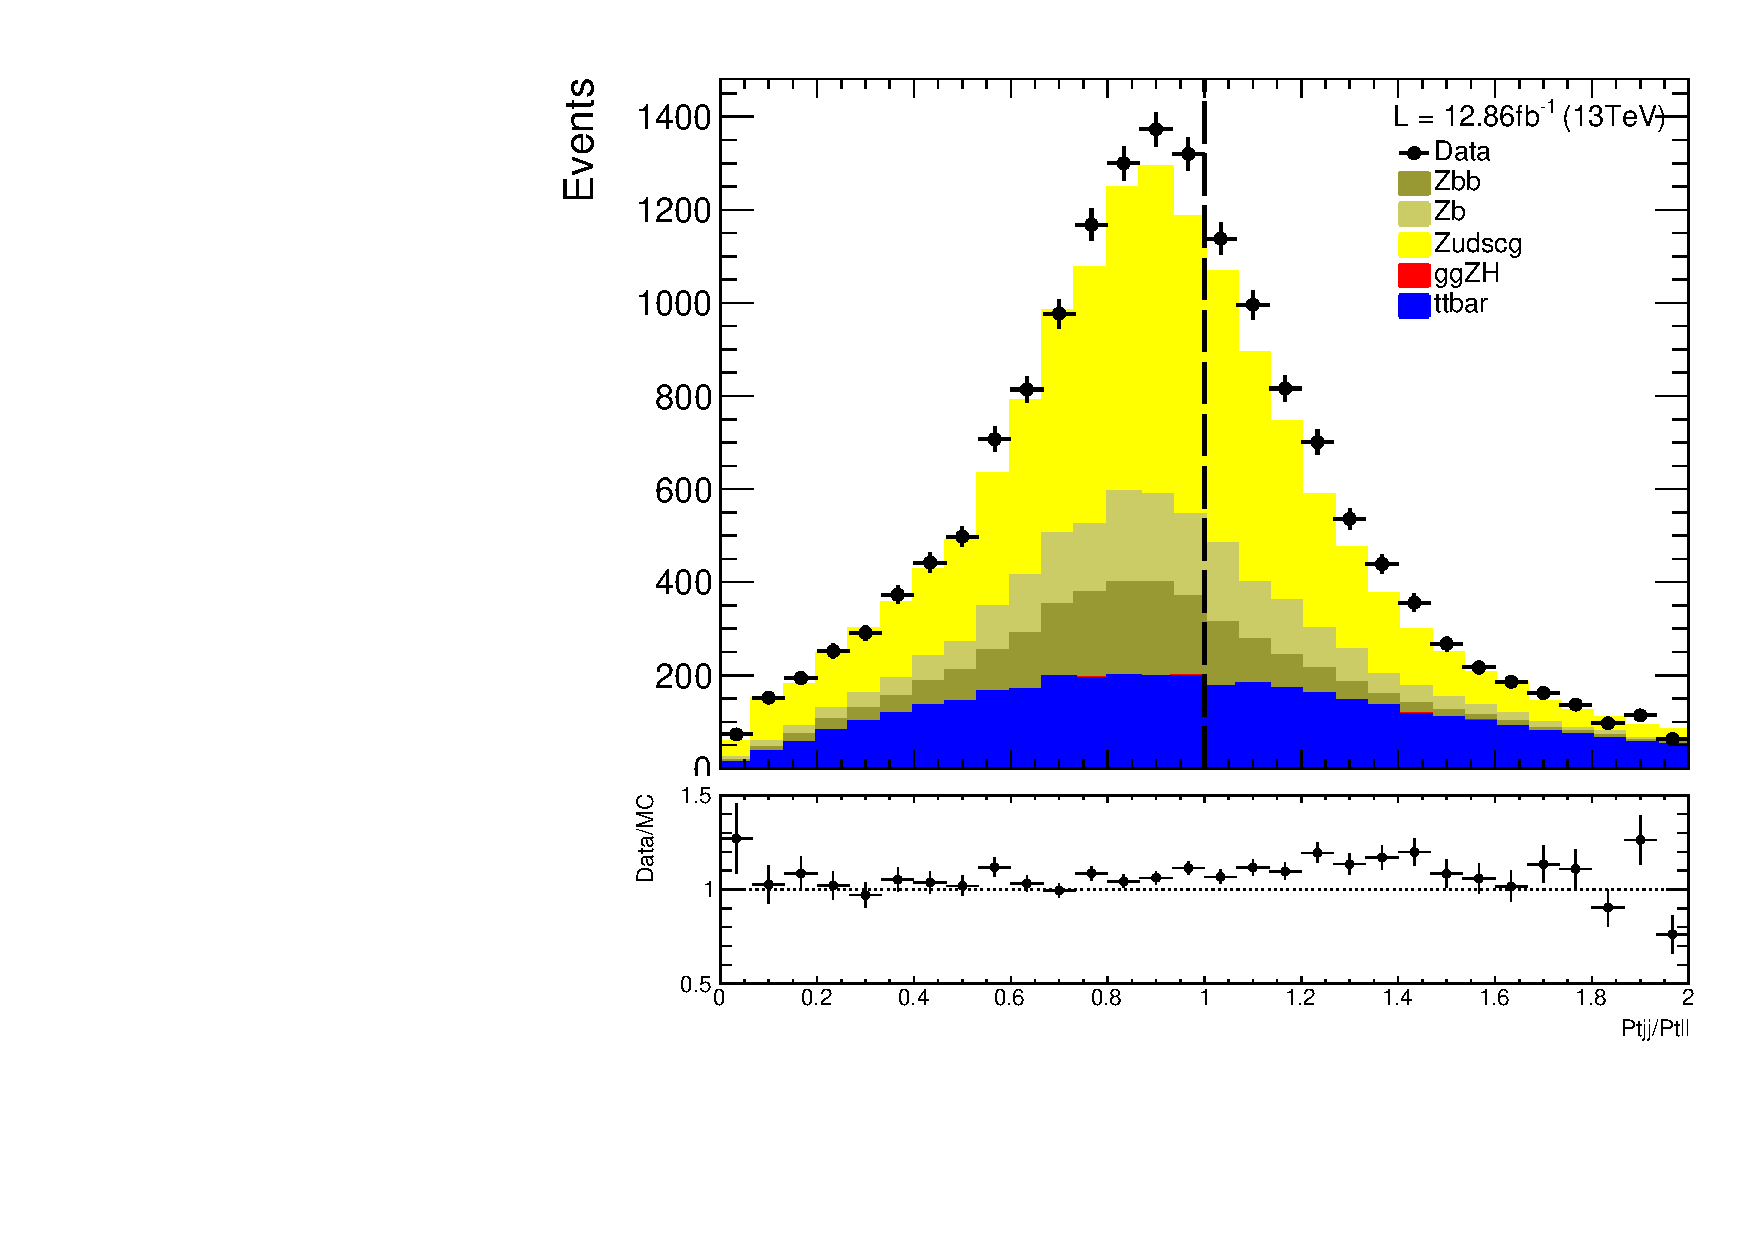
\includegraphics[width=0.32\textwidth]{b-reg/Vali_Data_MC_no_reg_PtBalance_mu_Loose}\hfil
  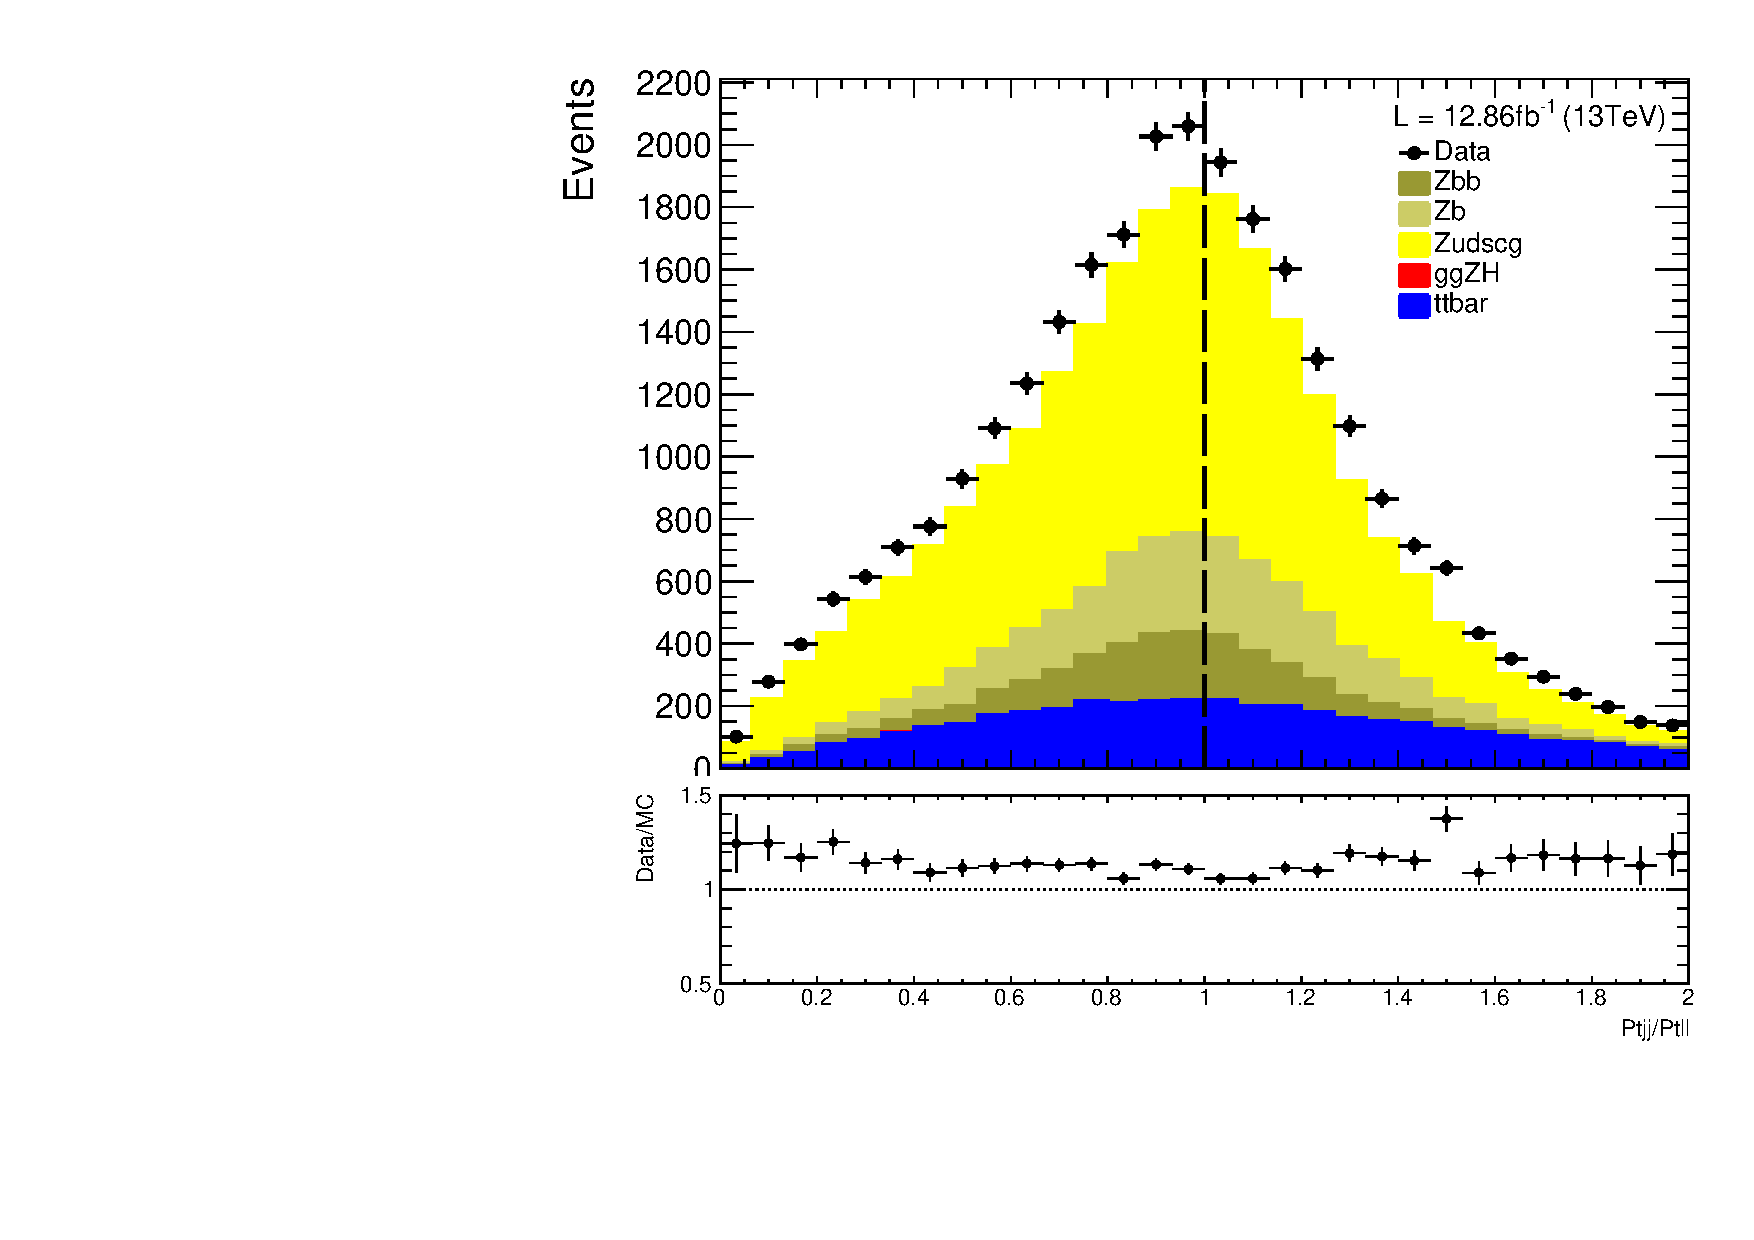
\includegraphics[width=0.32\textwidth]{b-reg/Vali_Data_MC_jet_16plus3_js_PtBalance_mu_Loose}\hfil
  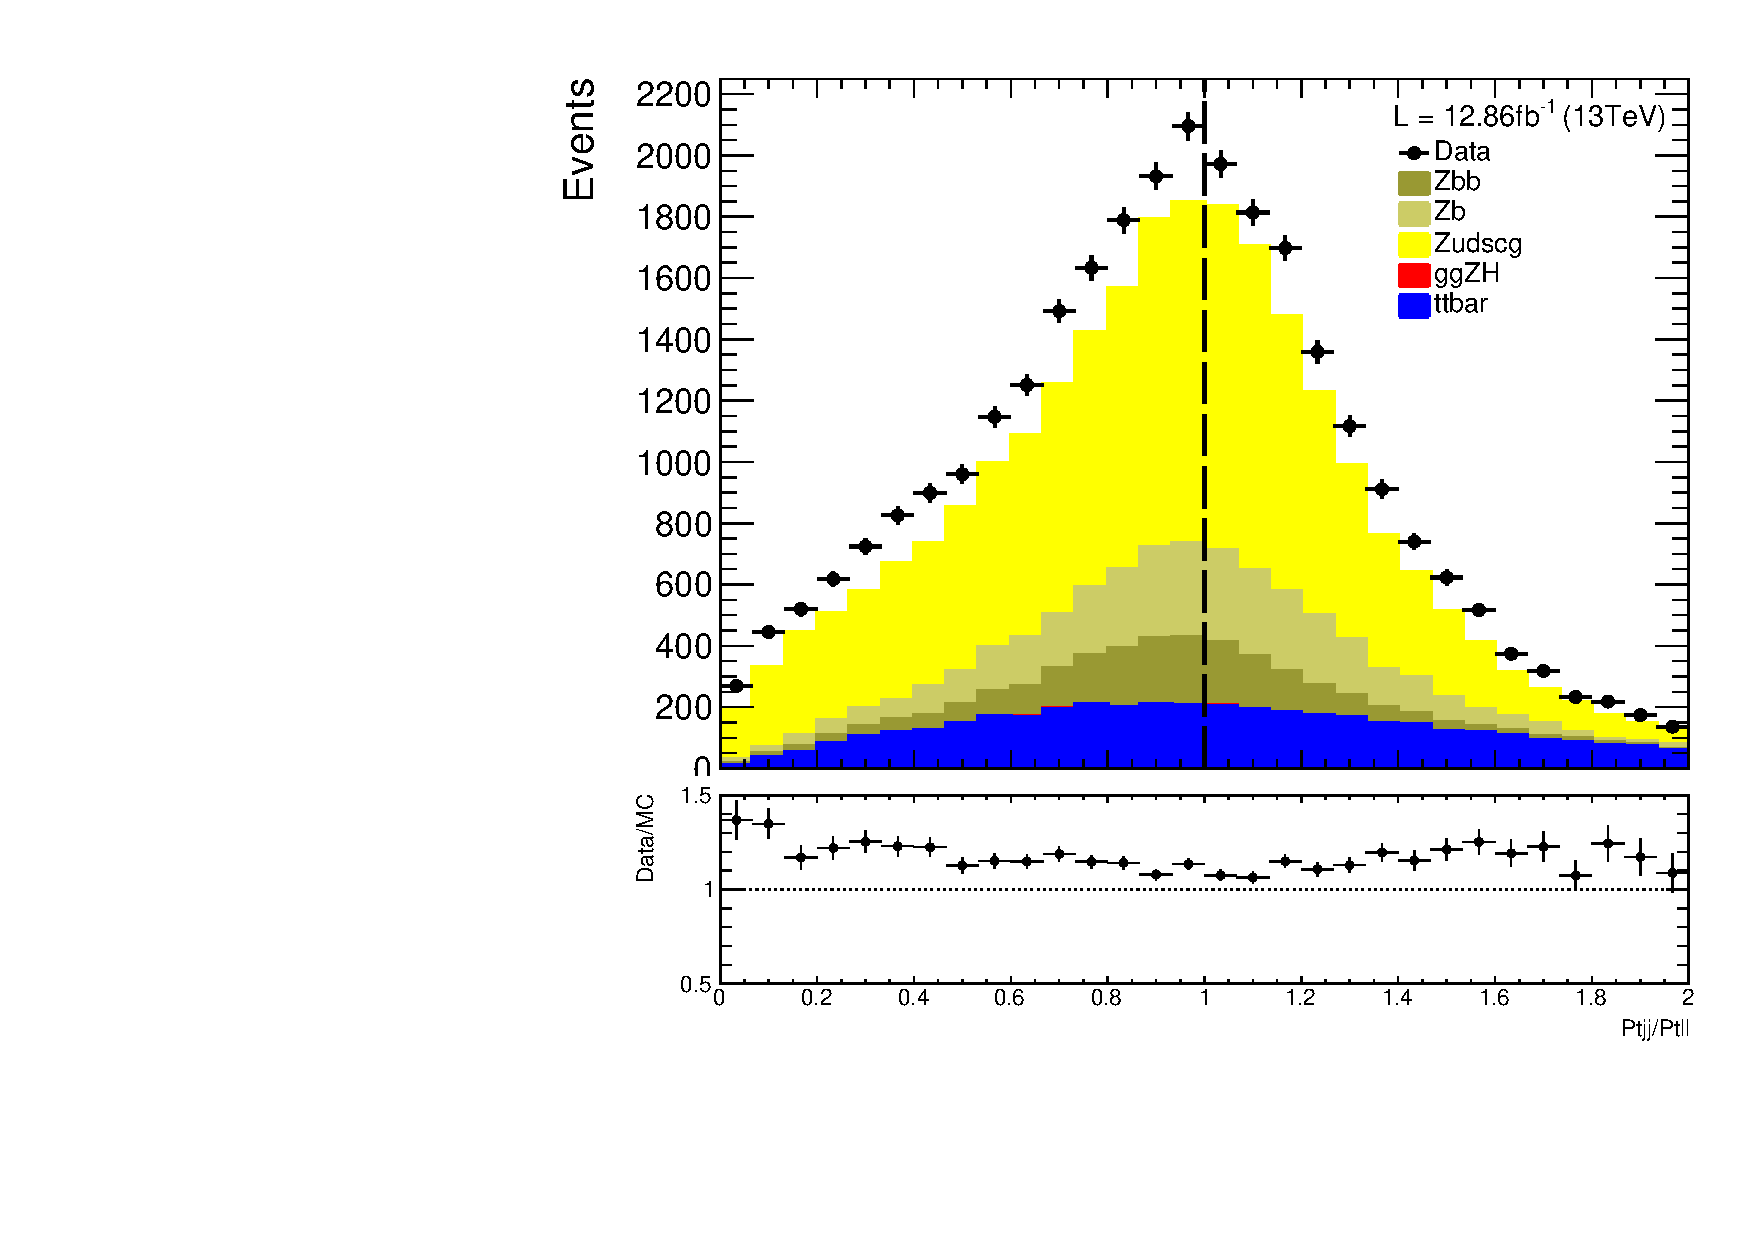
\includegraphics[width=0.32\textwidth]{b-reg/Vali_Data_MC_jet_Hbb_PtBalance_mu_Loose}\hfil\\
  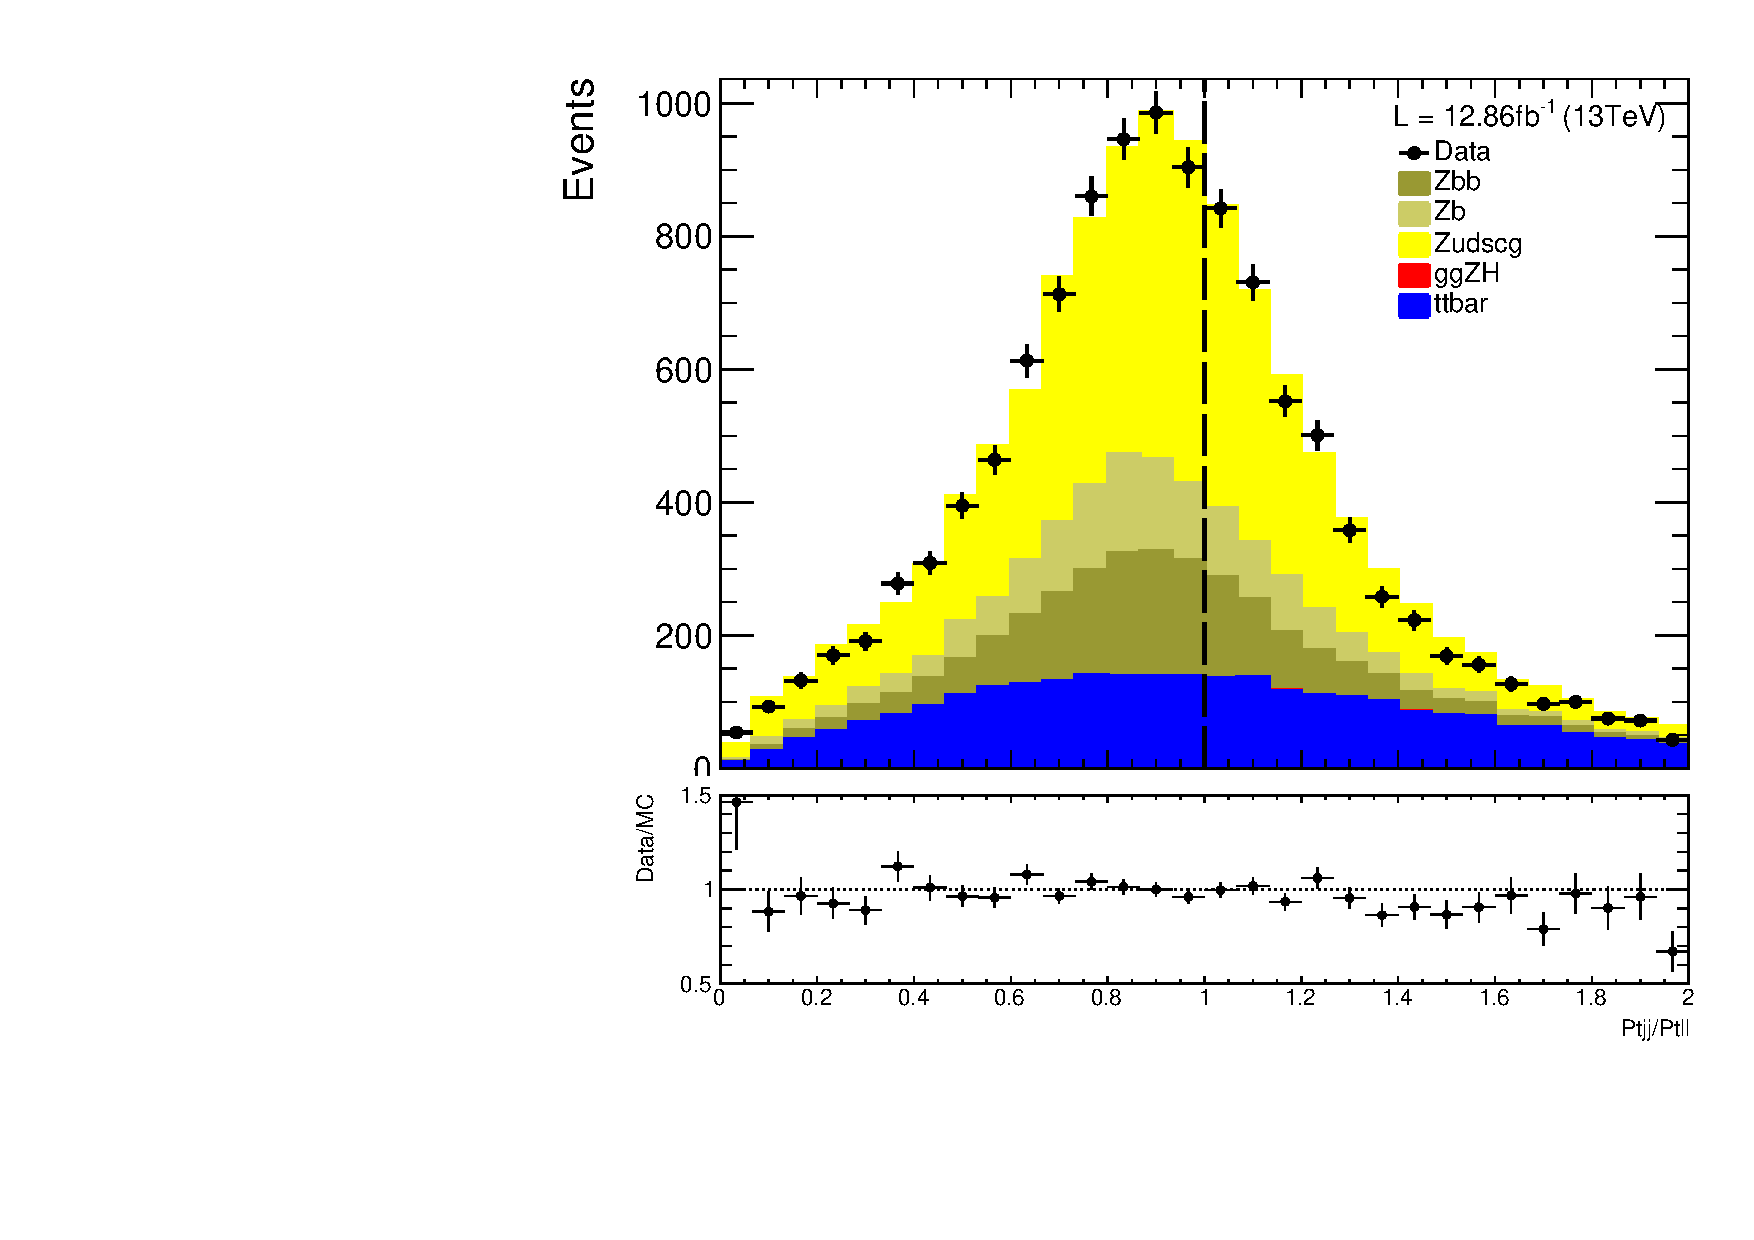
\includegraphics[width=0.32\textwidth]{b-reg/Vali_Data_MC_no_reg_PtBalance_ele_Loose}\hfil
  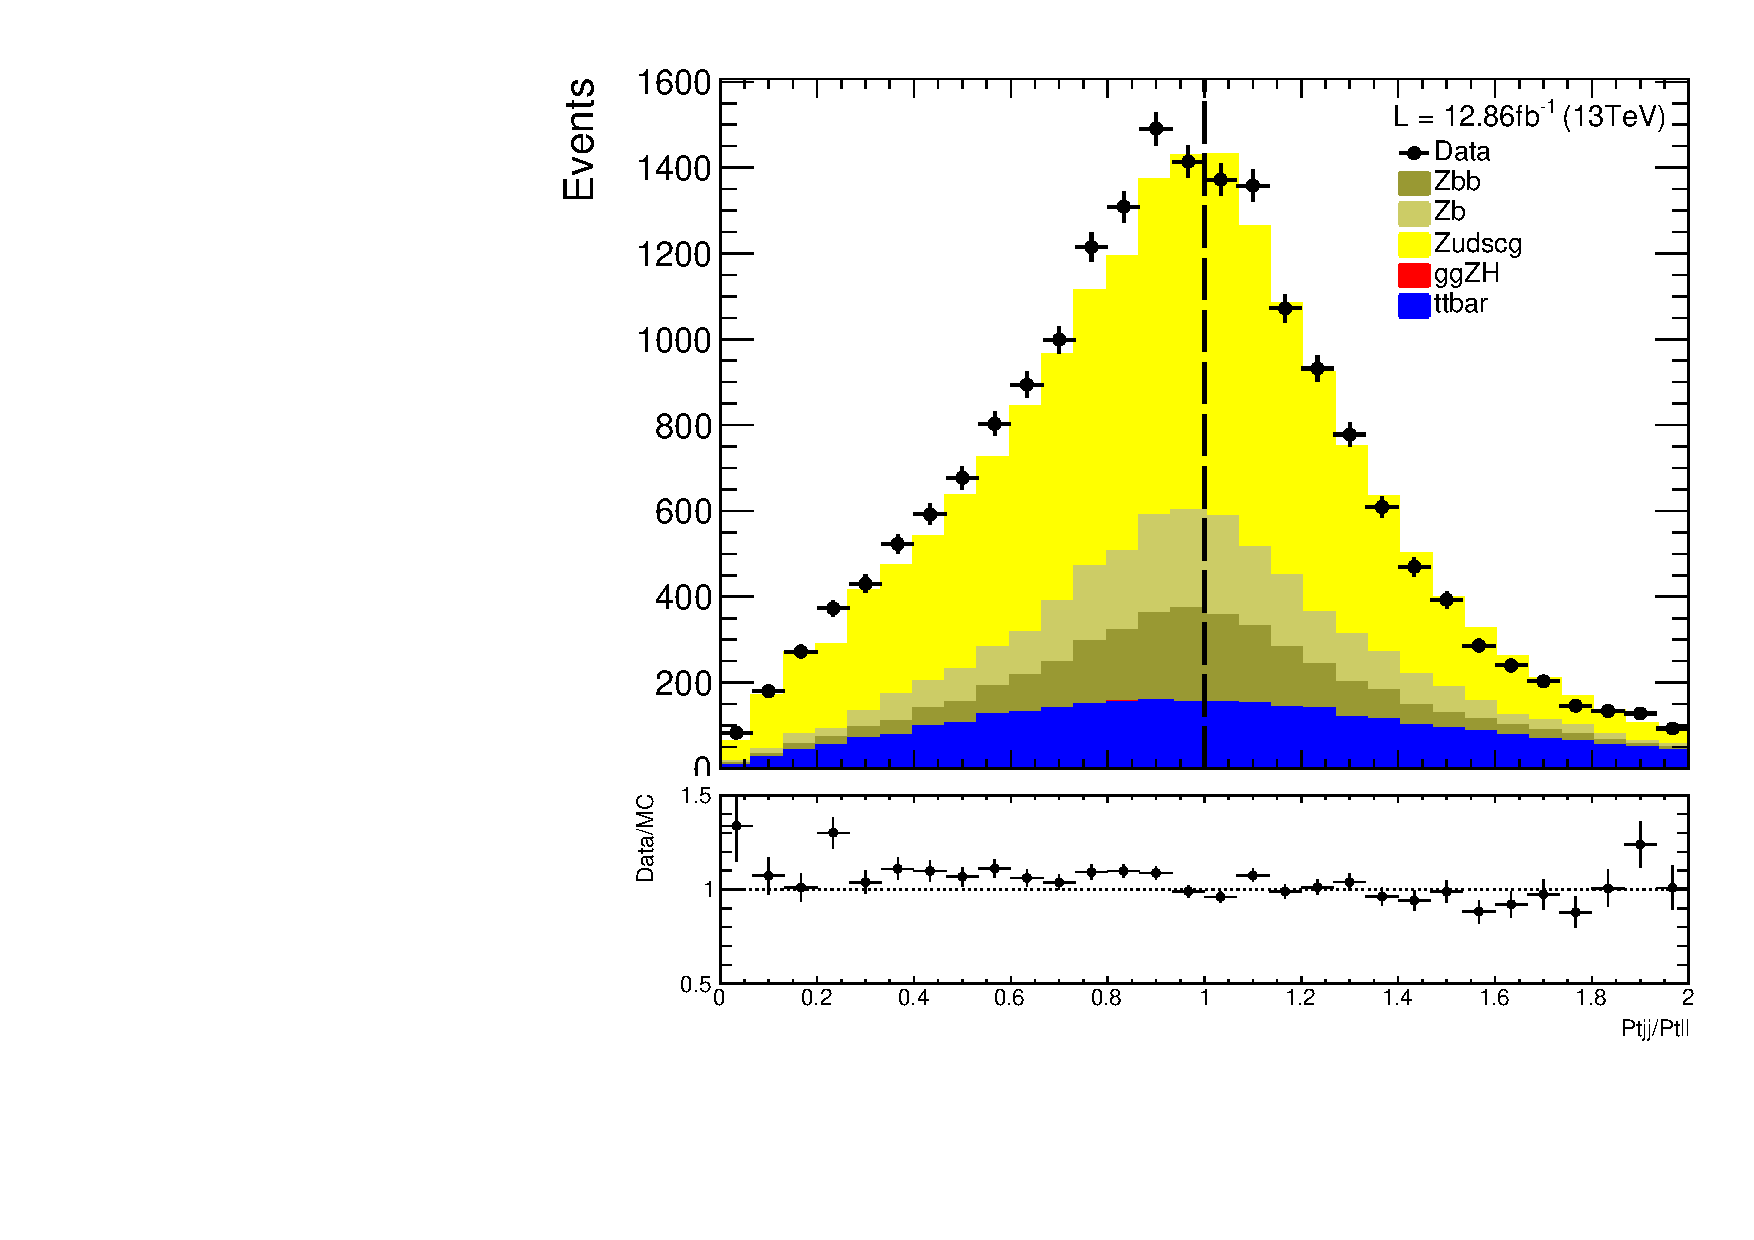
\includegraphics[width=0.32\textwidth]{b-reg/Vali_Data_MC_jet_16plus3_js_PtBalance_ele_Loose}\hfil
  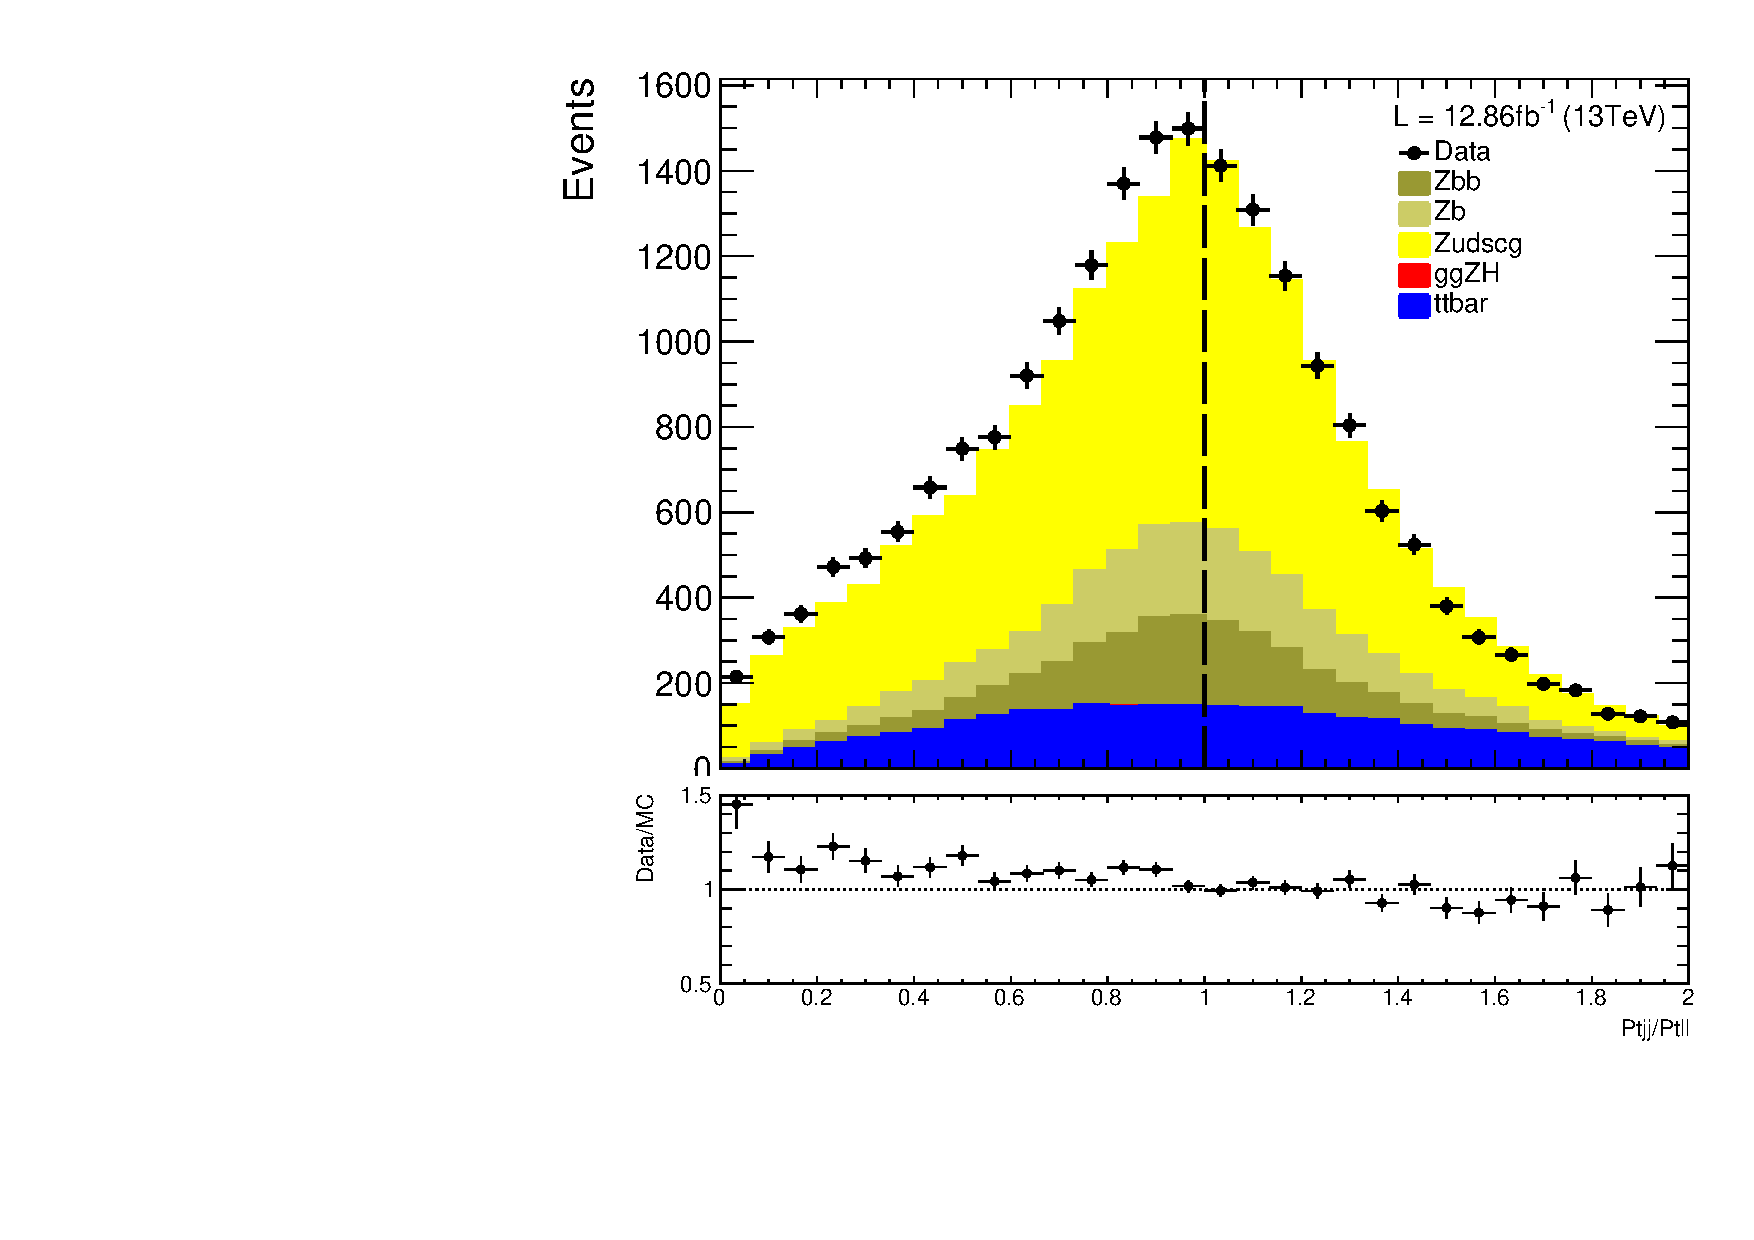
\includegraphics[width=0.32\textwidth]{b-reg/Vali_Data_MC_jet_Hbb_PtBalance_ele_Loose}\hfil\\
  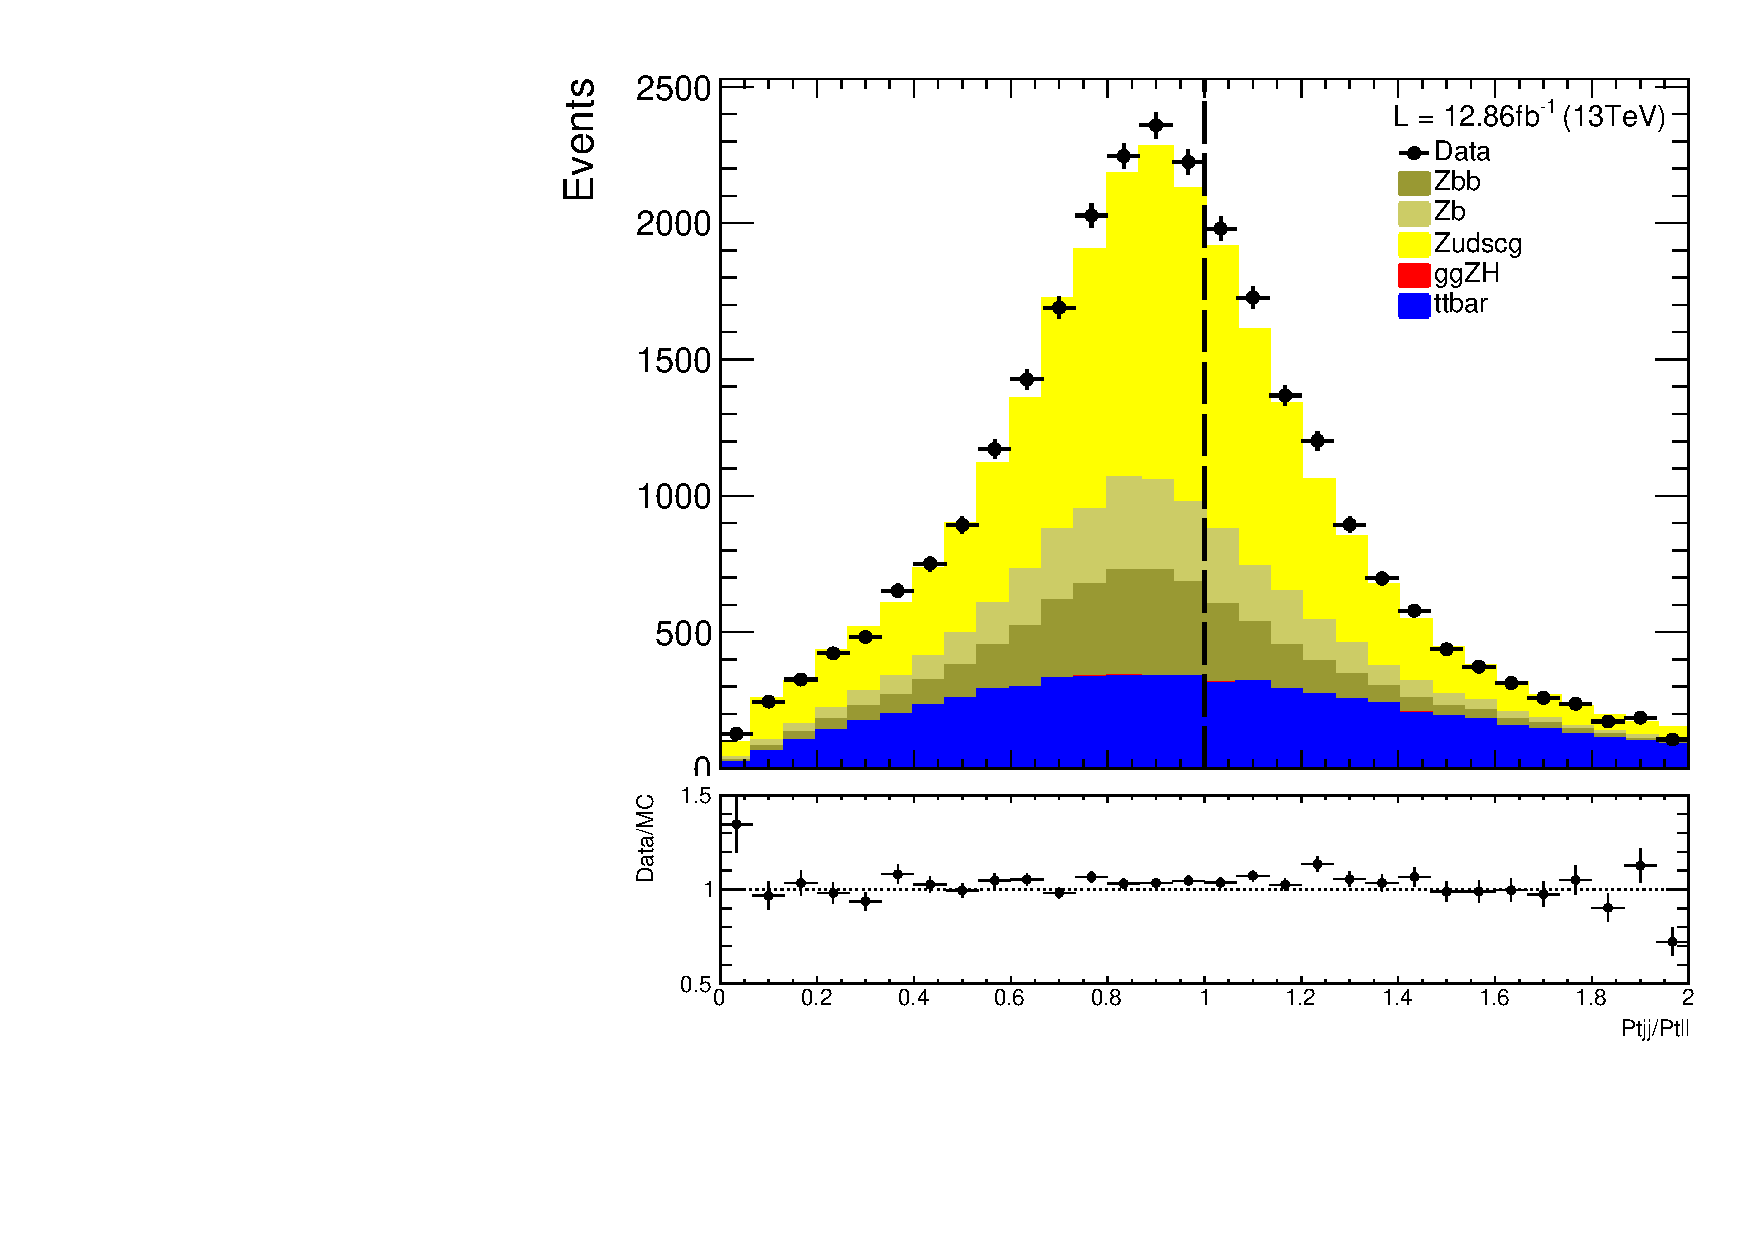
\includegraphics[width=0.32\textwidth]{b-reg/Vali_Data_MC_no_reg_PtBalance_all_Loose}\hfil
  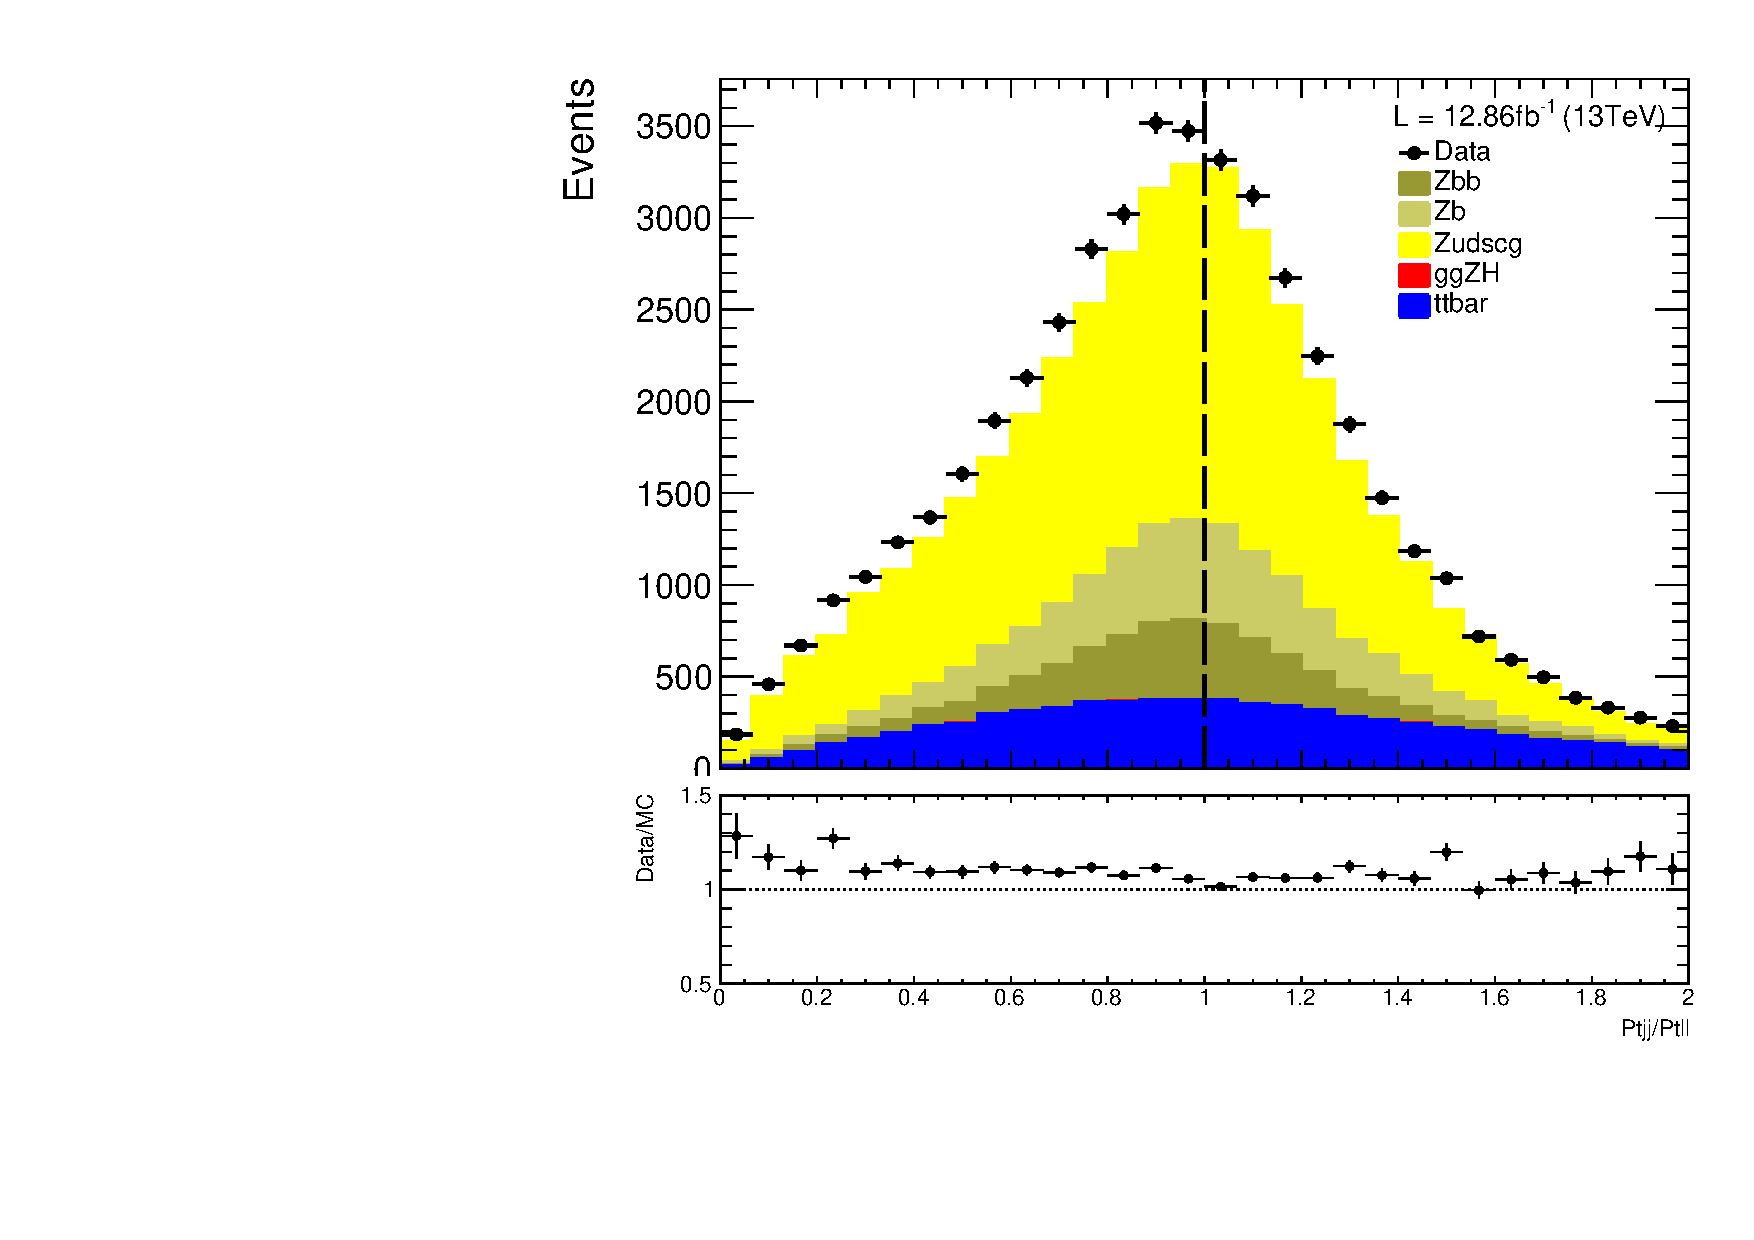
\includegraphics[width=0.32\textwidth]{b-reg/Vali_Data_MC_jet_16plus3_js_PtBalance_all_Loose}\hfil
  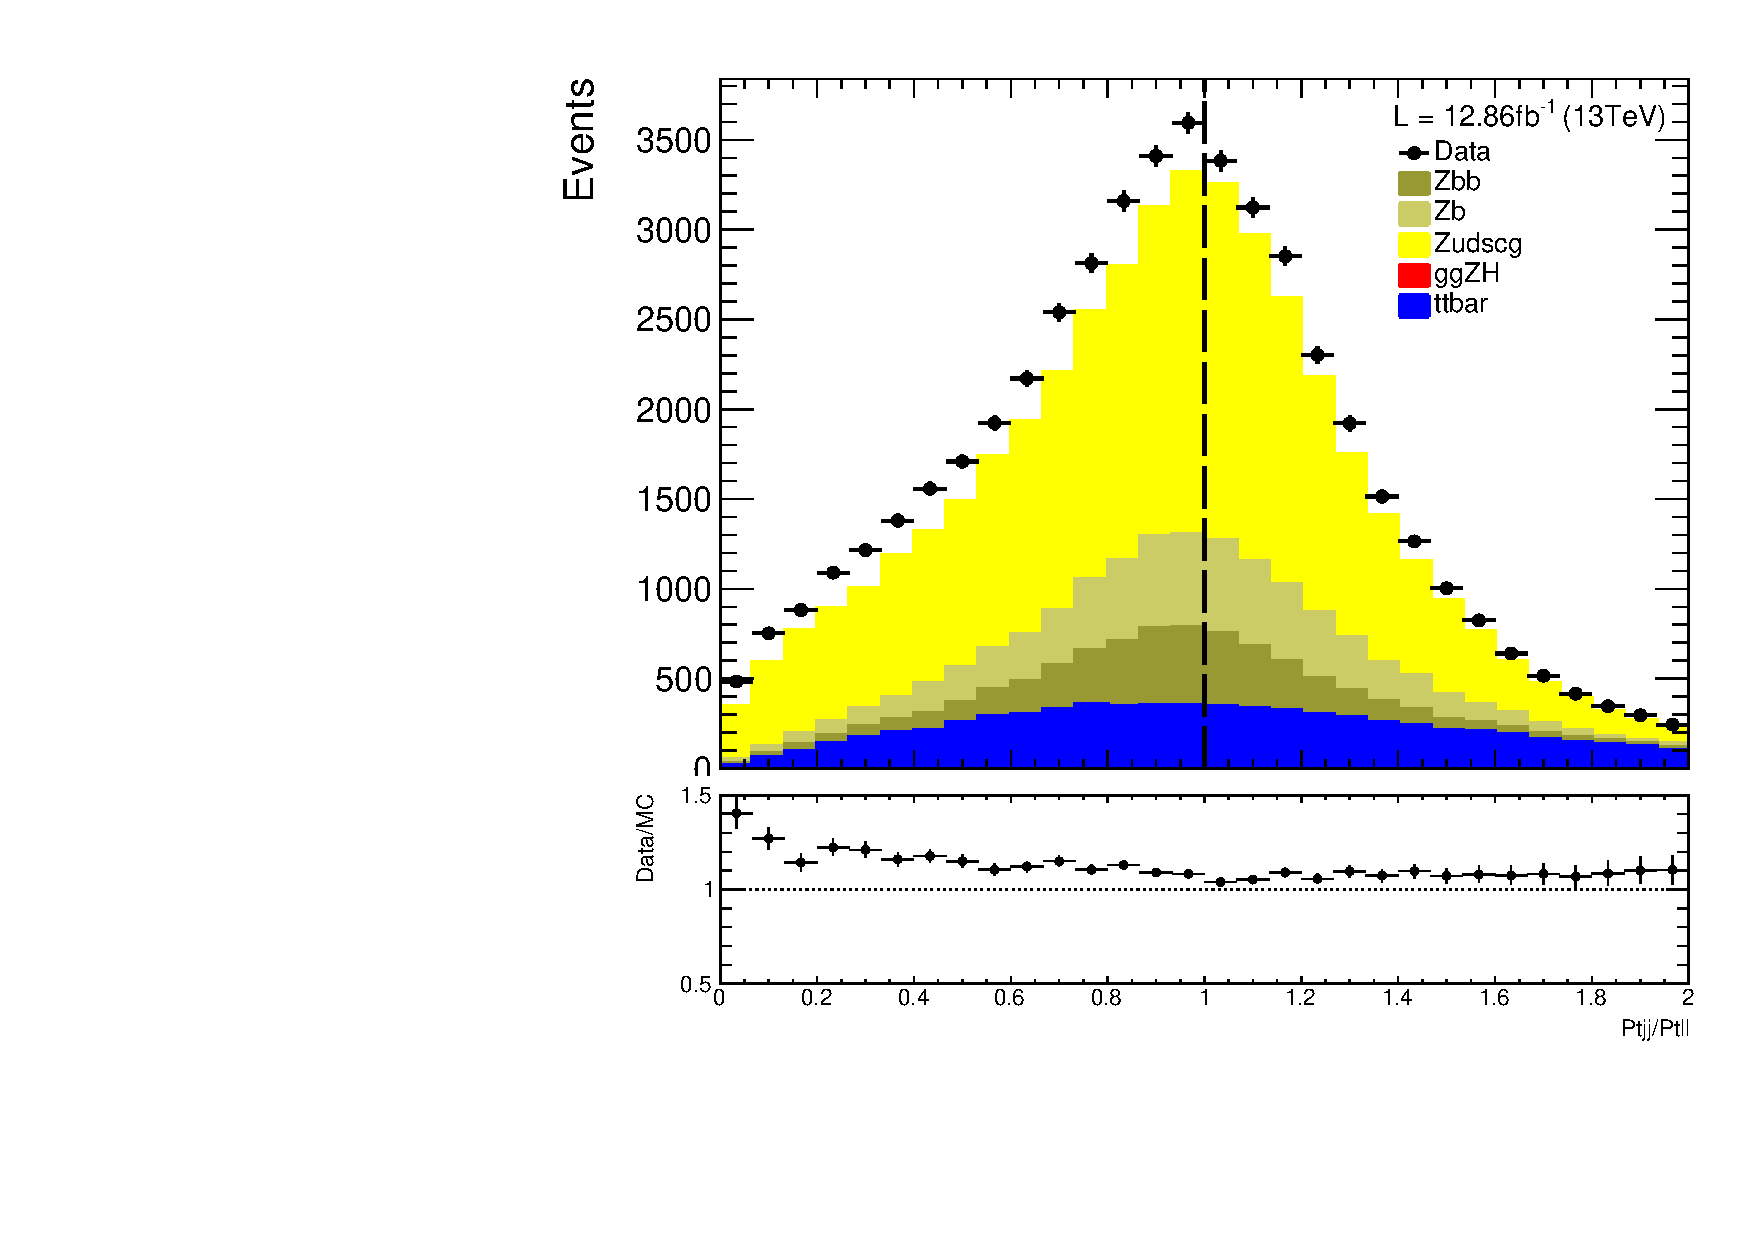
\includegraphics[width=0.32\textwidth]{b-reg/Vali_Data_MC_jet_Hbb_PtBalance_all_Loose}\hfil\\
  \caption{Pt balance (ratio) of the di-jet and di-lepton. On the left
    are plots with no regression, in the center - using
    \textbf{16plus3 js} training and on the right - using \textbf{Hbb}
    regression.  Top plots for muon channel, middle for electron
    channel and bottom is the combination (sum) of the two.  }
  \label{fig:vali-pt}
\end{figure*}


Figure \ref{fig:vali-pt} shows the mentioned $\PT$-balance
distributions, $\PT^{jj}/\PT^{\ell\ell}$.  The data is compared to the
MC predictions. It can be seen that before any regression is applied
(left plots) the peak of the ratio distribution is below one. With the
regression applied the peak moves to 1 for both our \textbf{16plus3
  js} training (center) and the one from \textbf{Hbb} (right). The
trend is the same in data and MC.  This indicates that the regression
does indeed brings the $\PT$ of the $b$-jets closer to their true
values.

Similarly, figure~\ref{fig:vali-Mjj} shows the mass distributions,
$m_{jj}$, before and after regression. These figures indicate that
$m_{jj}$ is not distorted in any bad way, no artificial peaks are
created. This ensures us that the background distributions in our
analysis signal region will not be distorted either.

\begin{figure*}[thb]
  \centering
  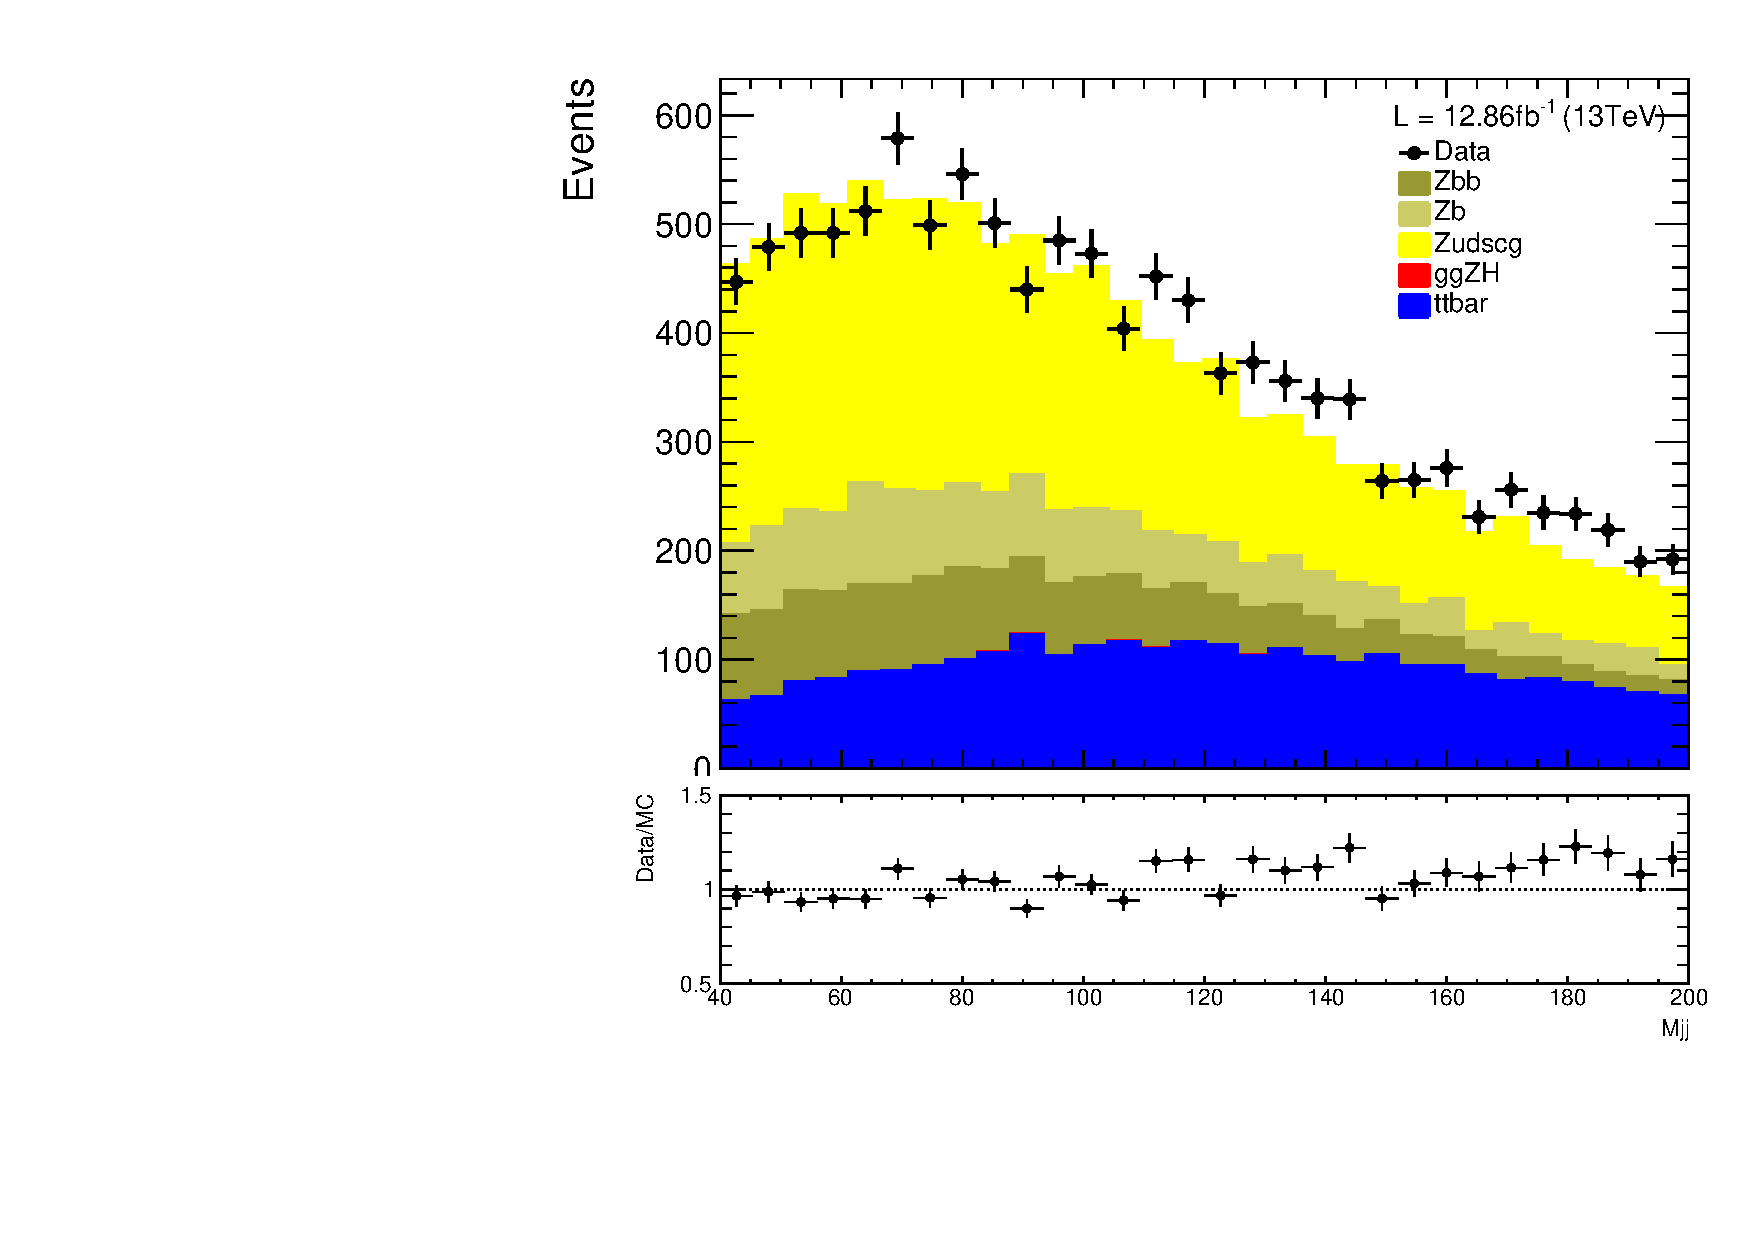
\includegraphics[width=0.32\textwidth]{b-reg/Vali_Data_MC_no_reg_Mjj_mu_Loose}\hfil
  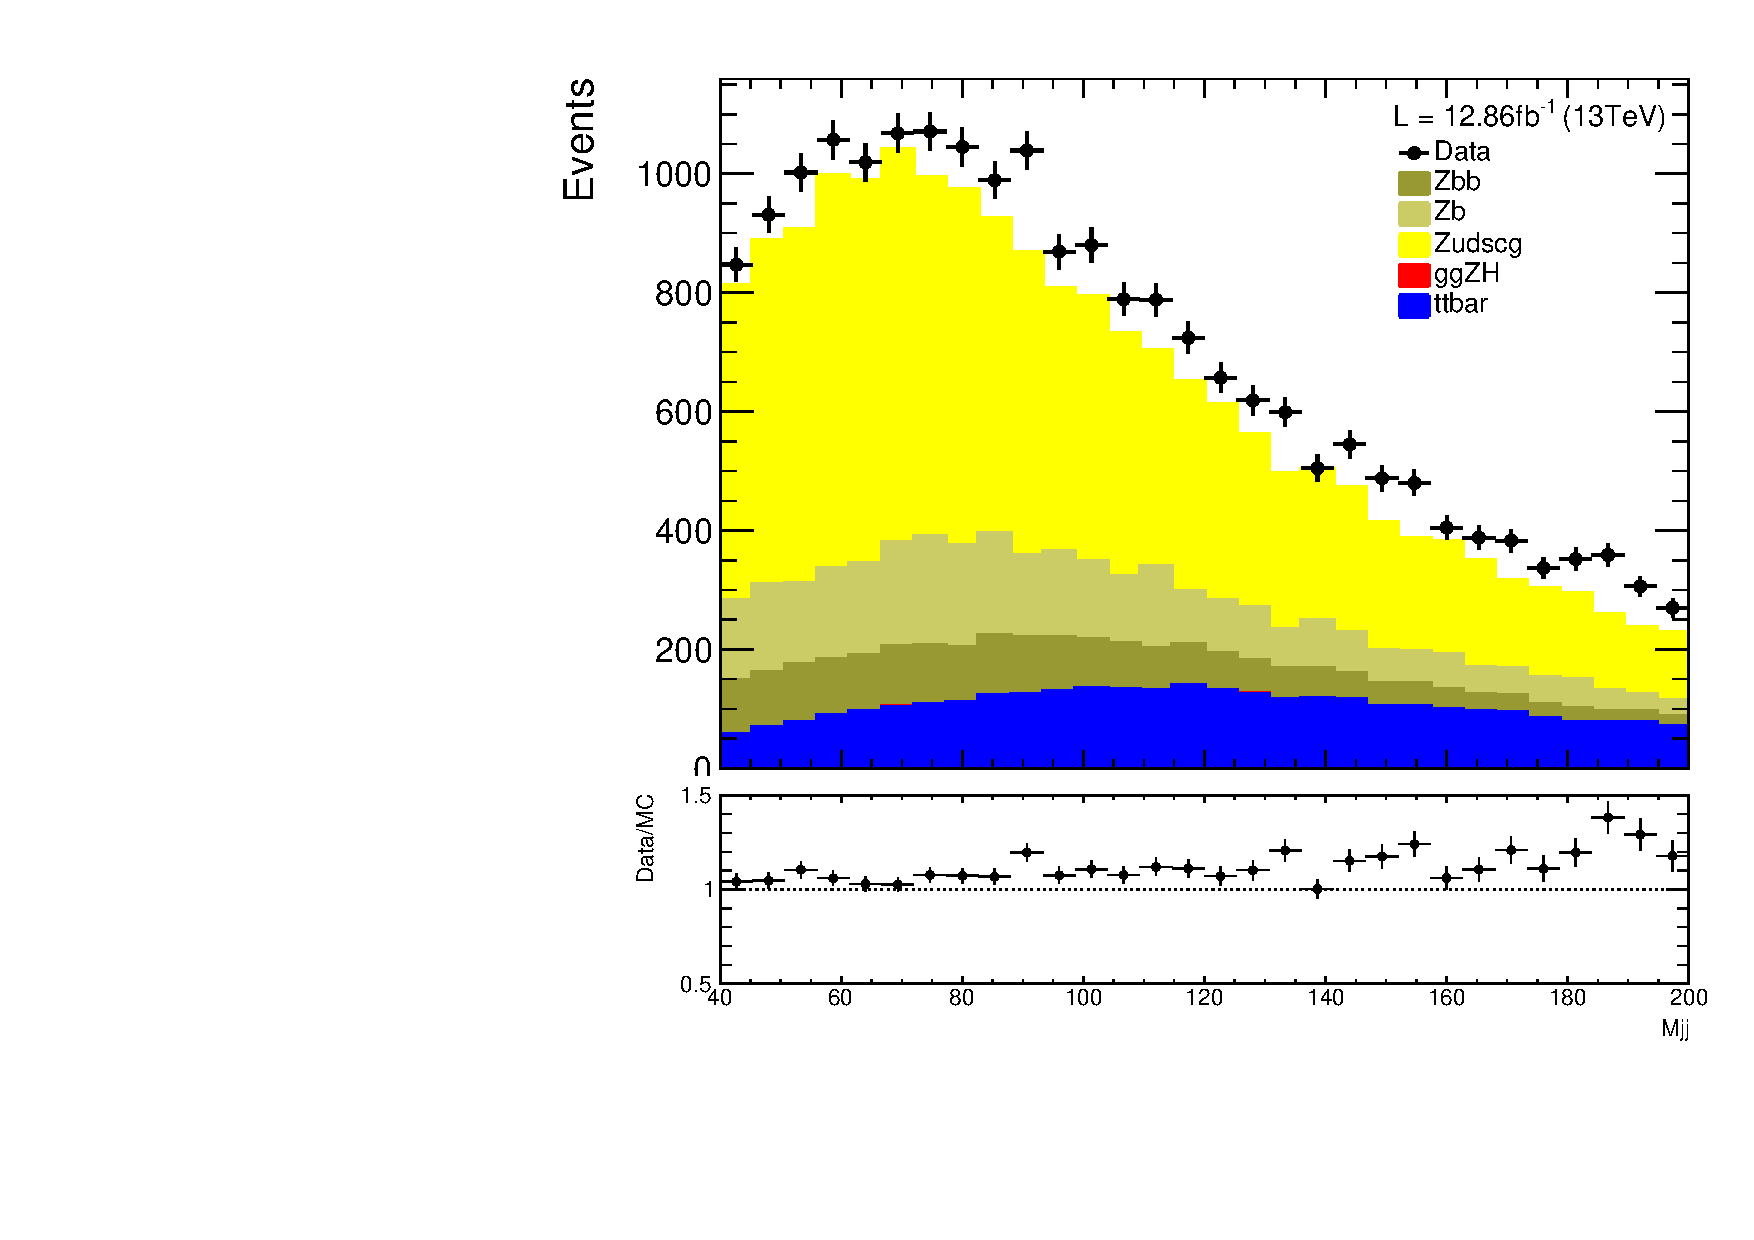
\includegraphics[width=0.32\textwidth]{b-reg/Vali_Data_MC_jet_16plus3_js_Mjj_mu_Loose}\hfil
  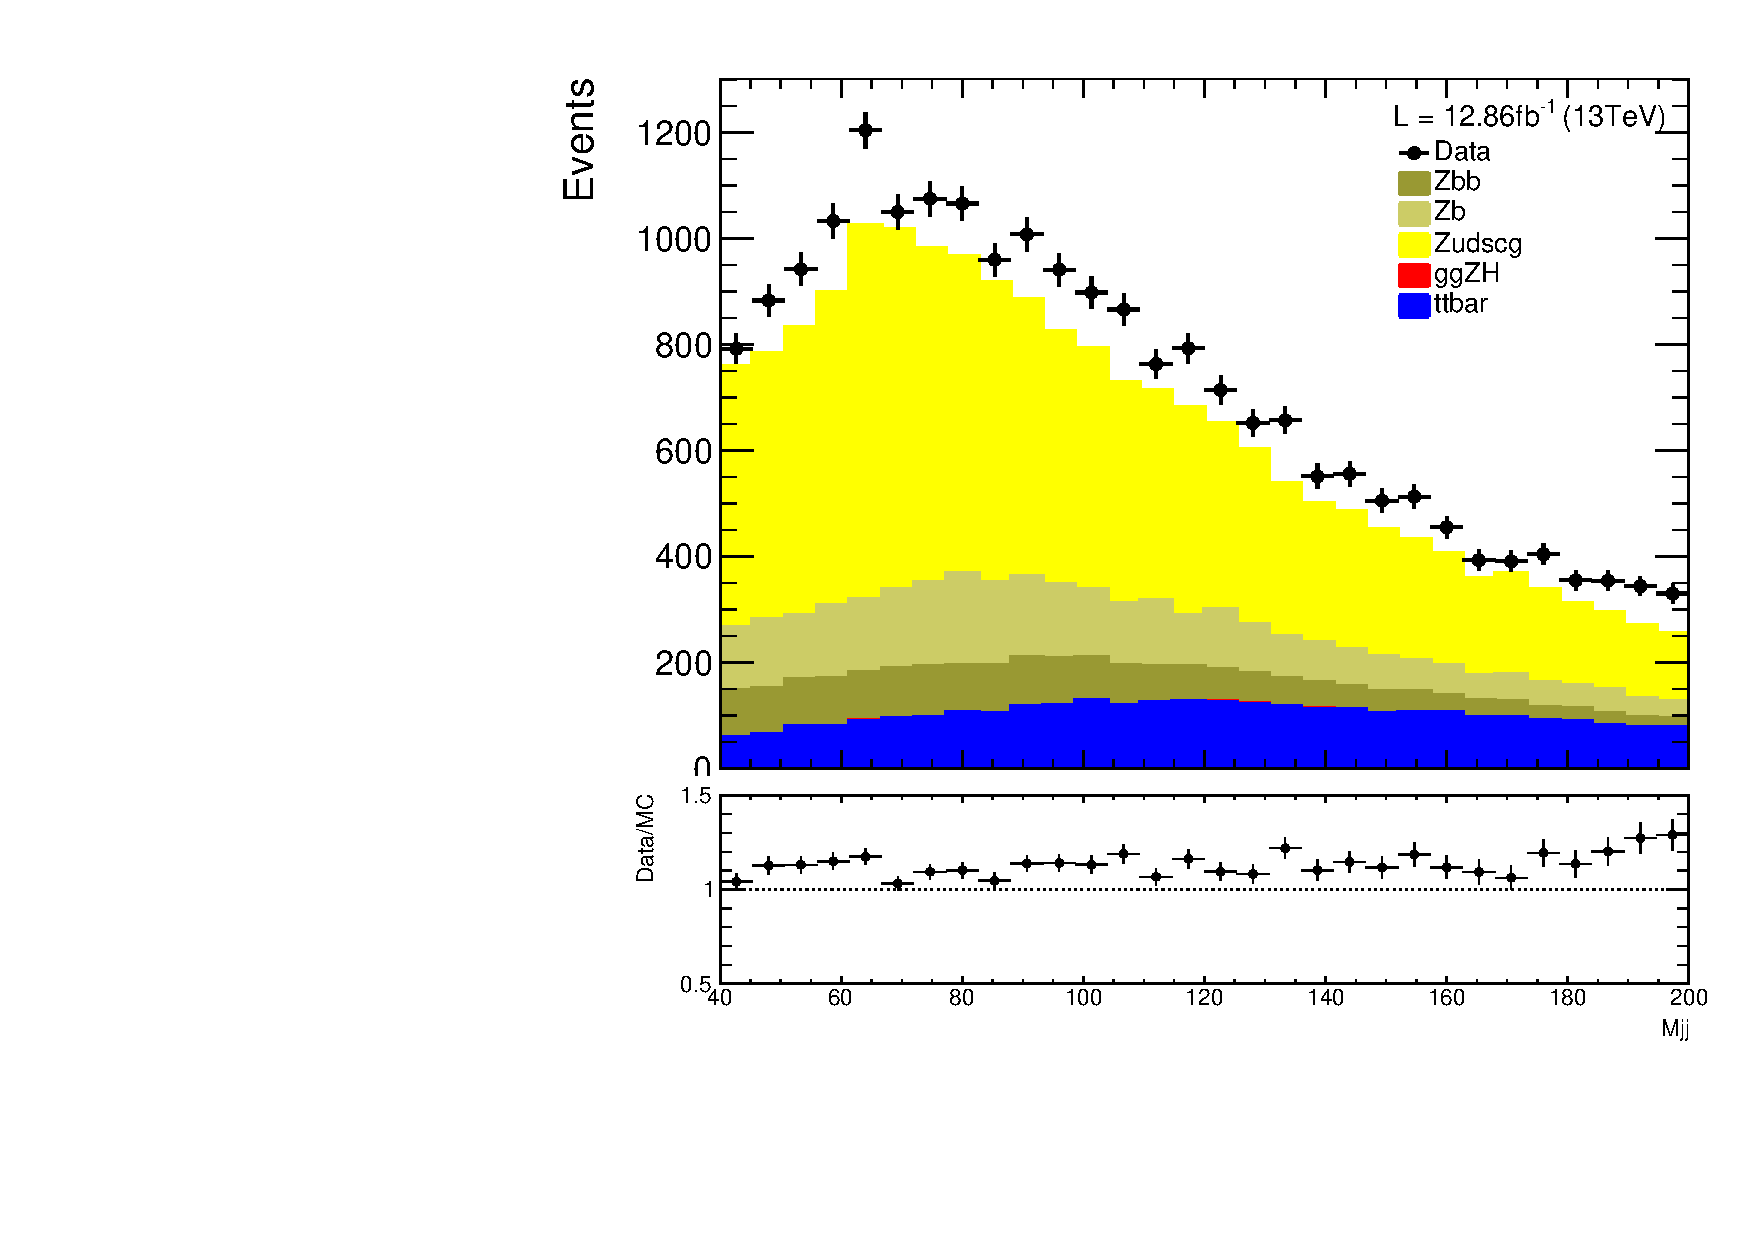
\includegraphics[width=0.32\textwidth]{b-reg/Vali_Data_MC_jet_Hbb_Mjj_mu_Loose}\hfil\\
  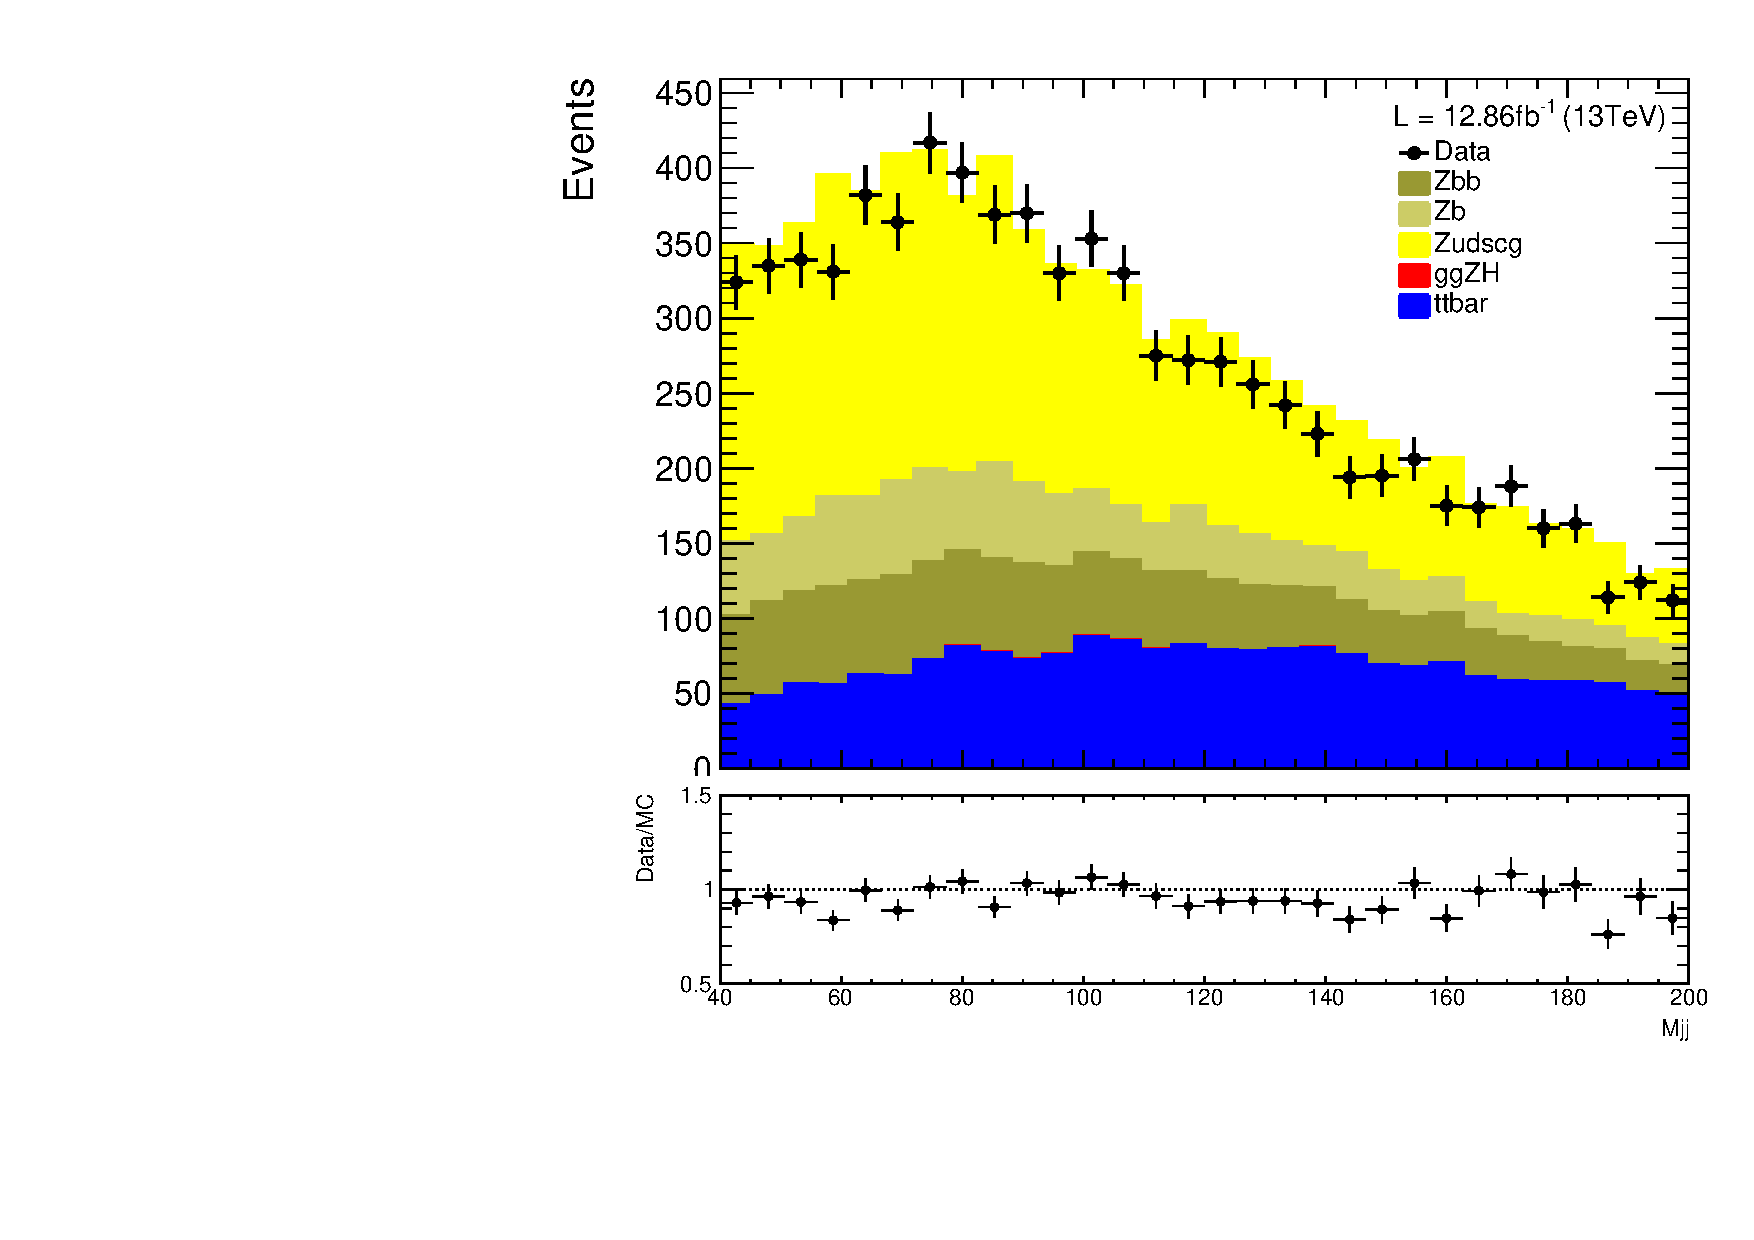
\includegraphics[width=0.32\textwidth]{b-reg/Vali_Data_MC_no_reg_Mjj_ele_Loose}\hfil
  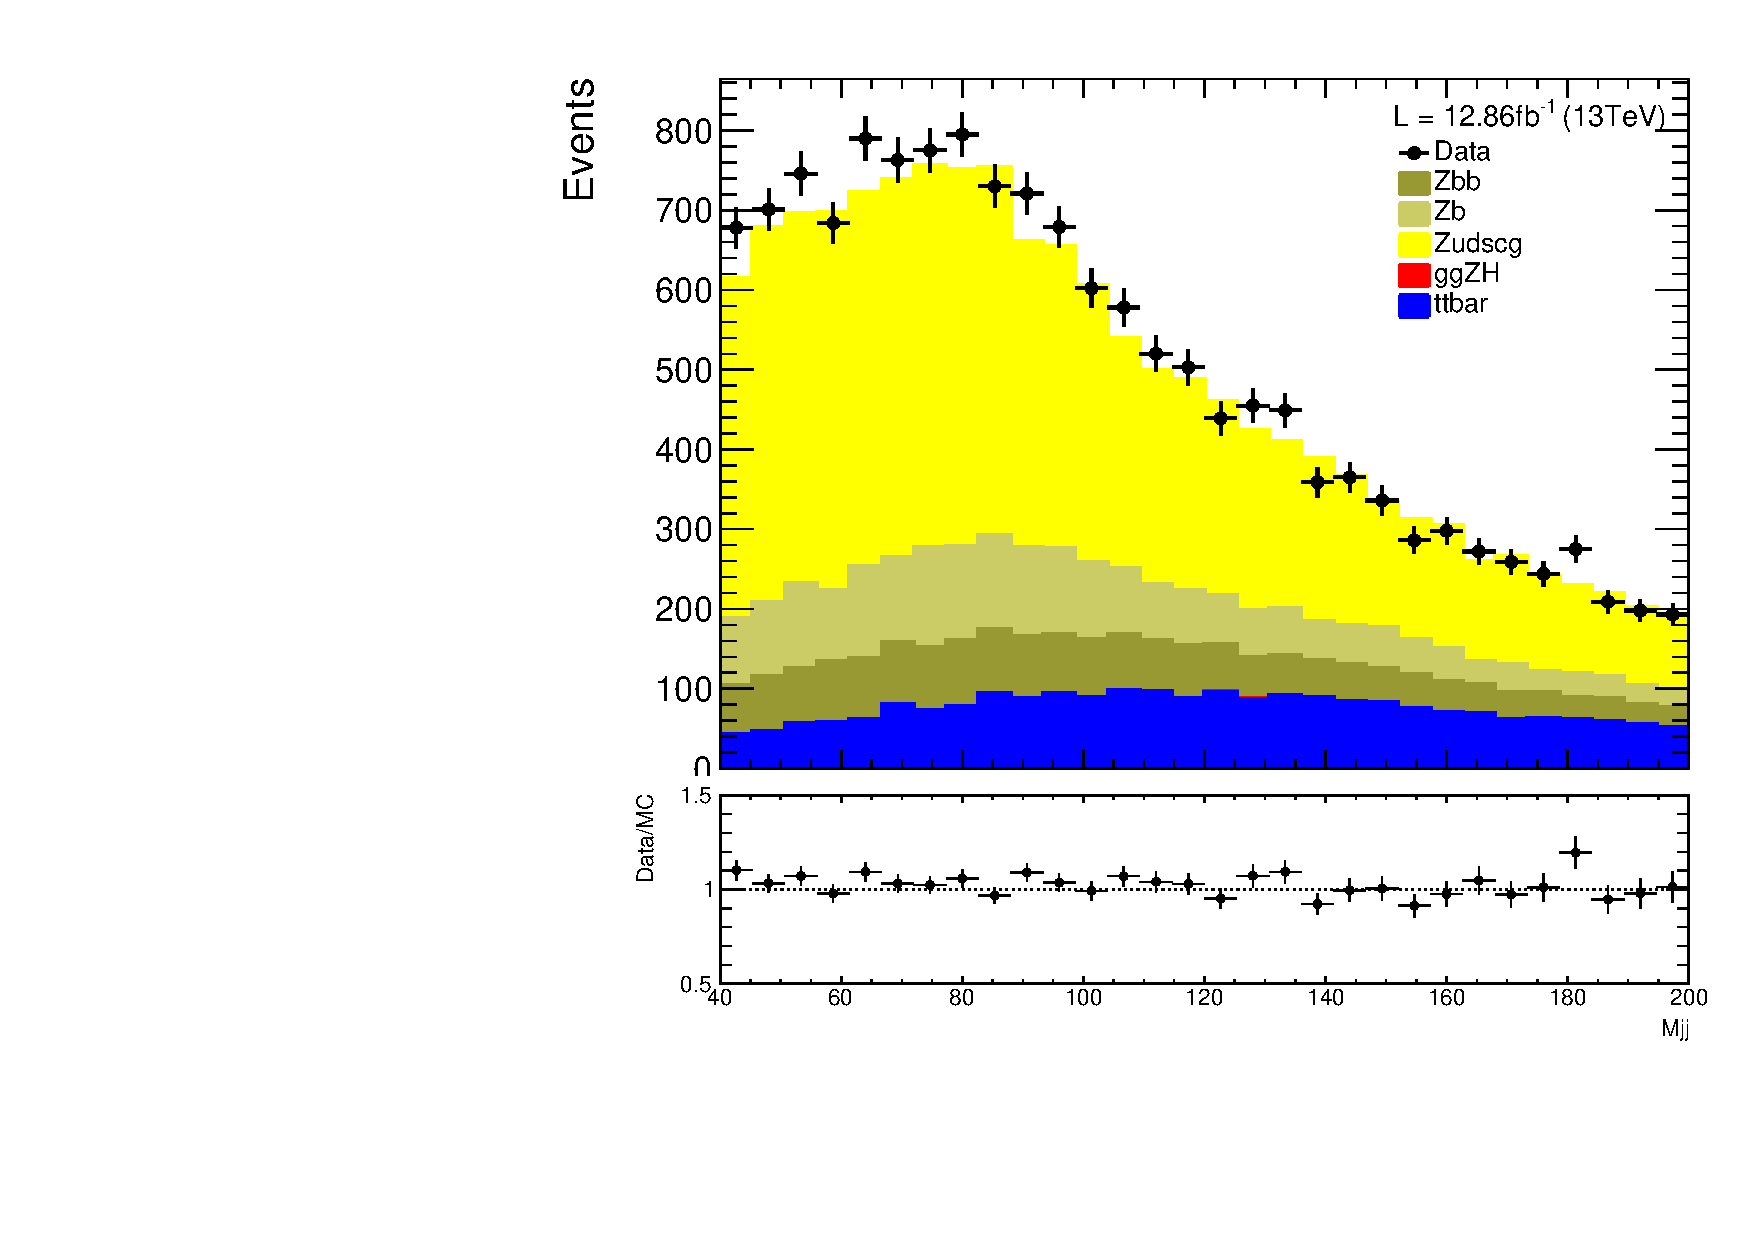
\includegraphics[width=0.32\textwidth]{b-reg/Vali_Data_MC_jet_16plus3_js_Mjj_ele_Loose}\hfil
  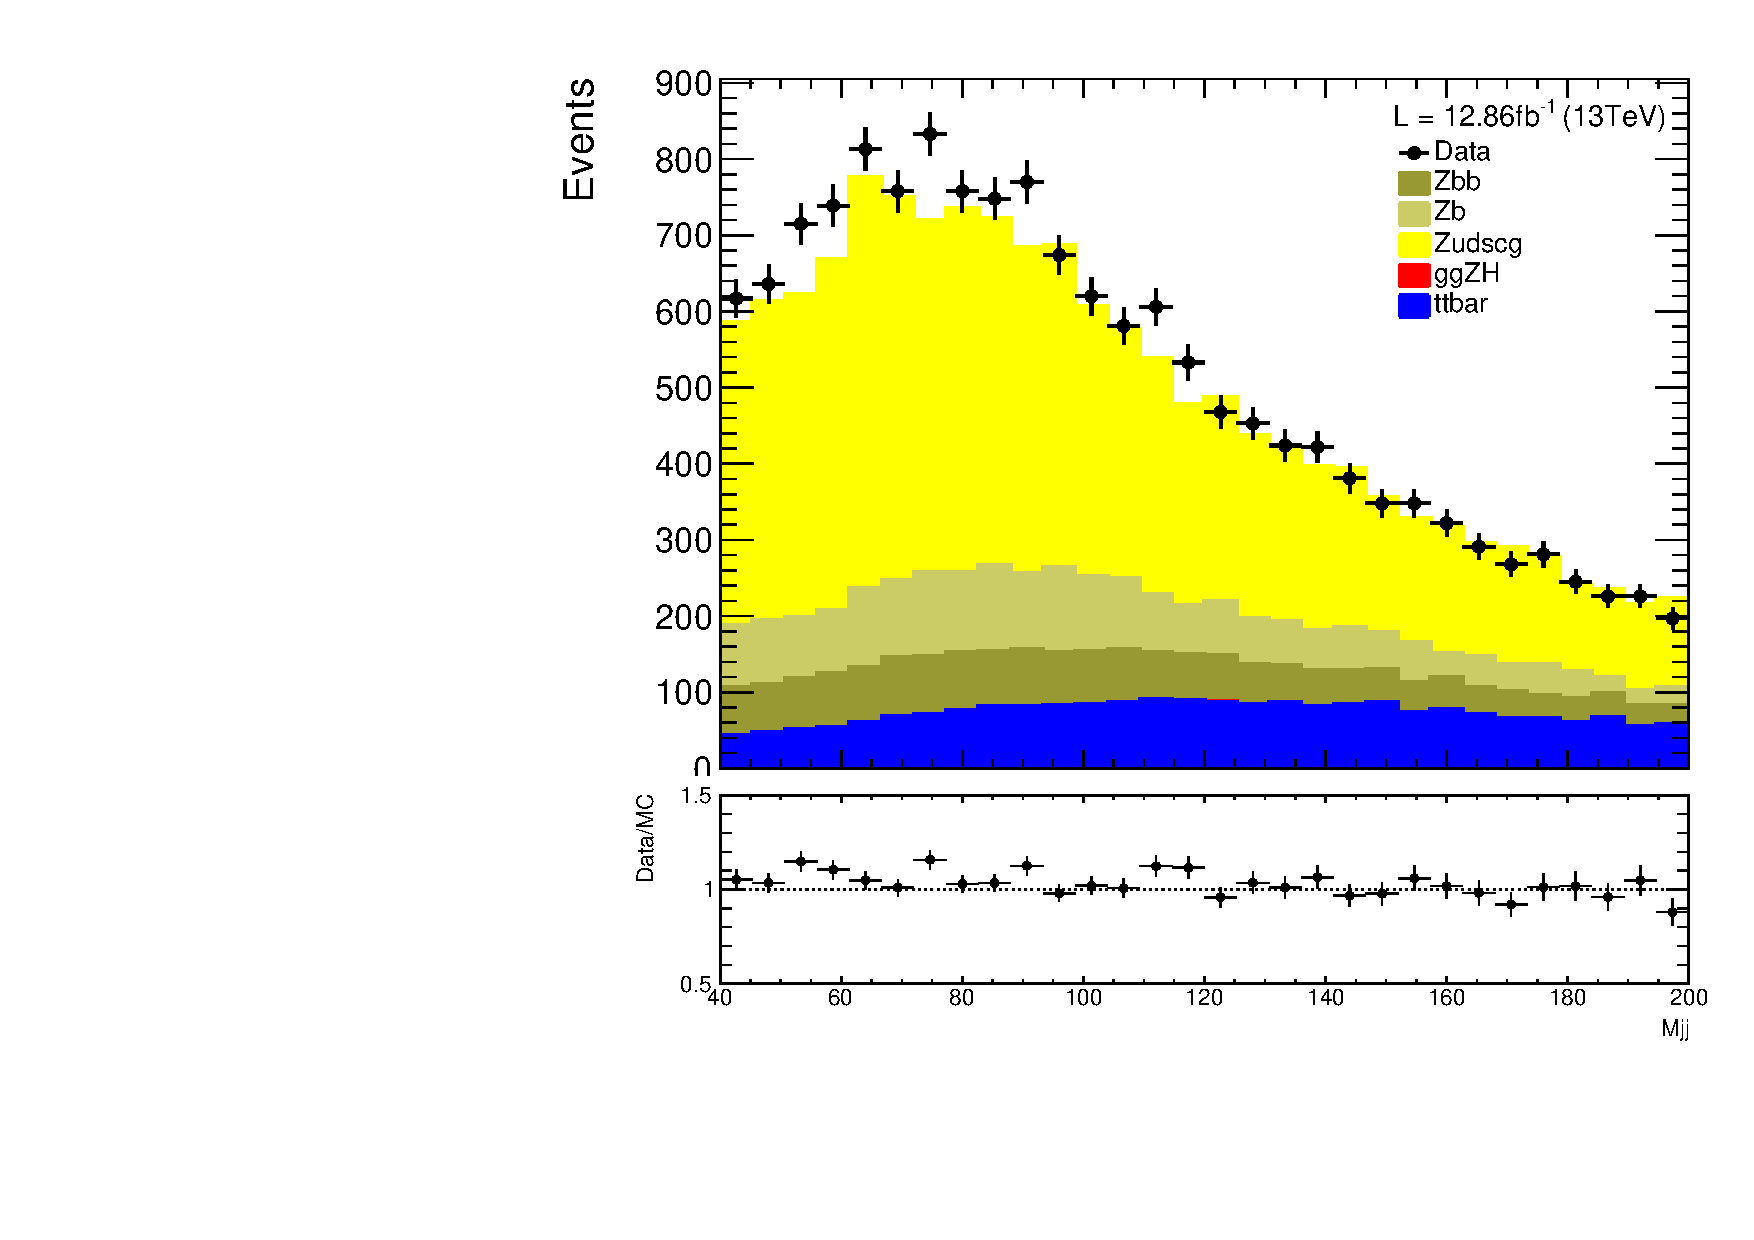
\includegraphics[width=0.32\textwidth]{b-reg/Vali_Data_MC_jet_Hbb_Mjj_ele_Loose}\hfil\\
  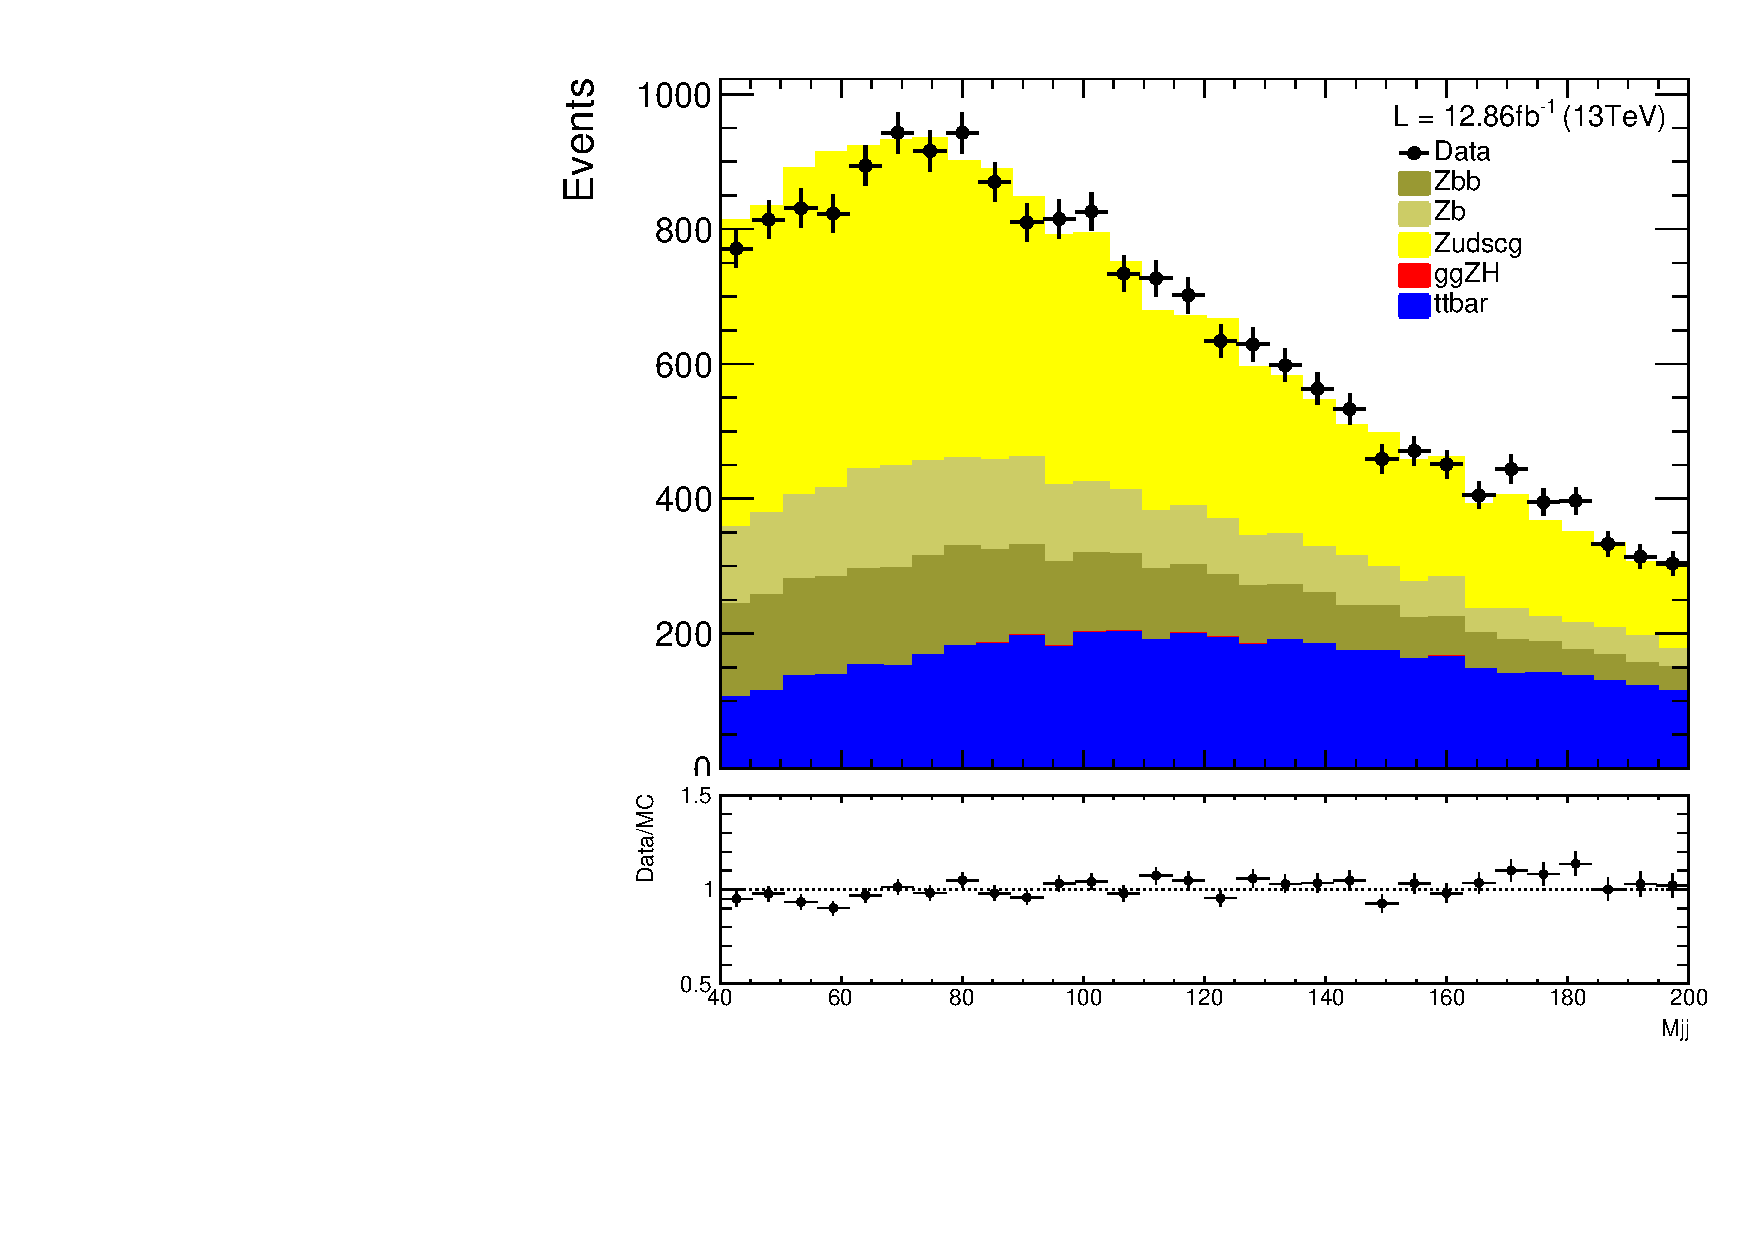
\includegraphics[width=0.32\textwidth]{b-reg/Vali_Data_MC_no_reg_Mjj_all_Loose}\hfil
  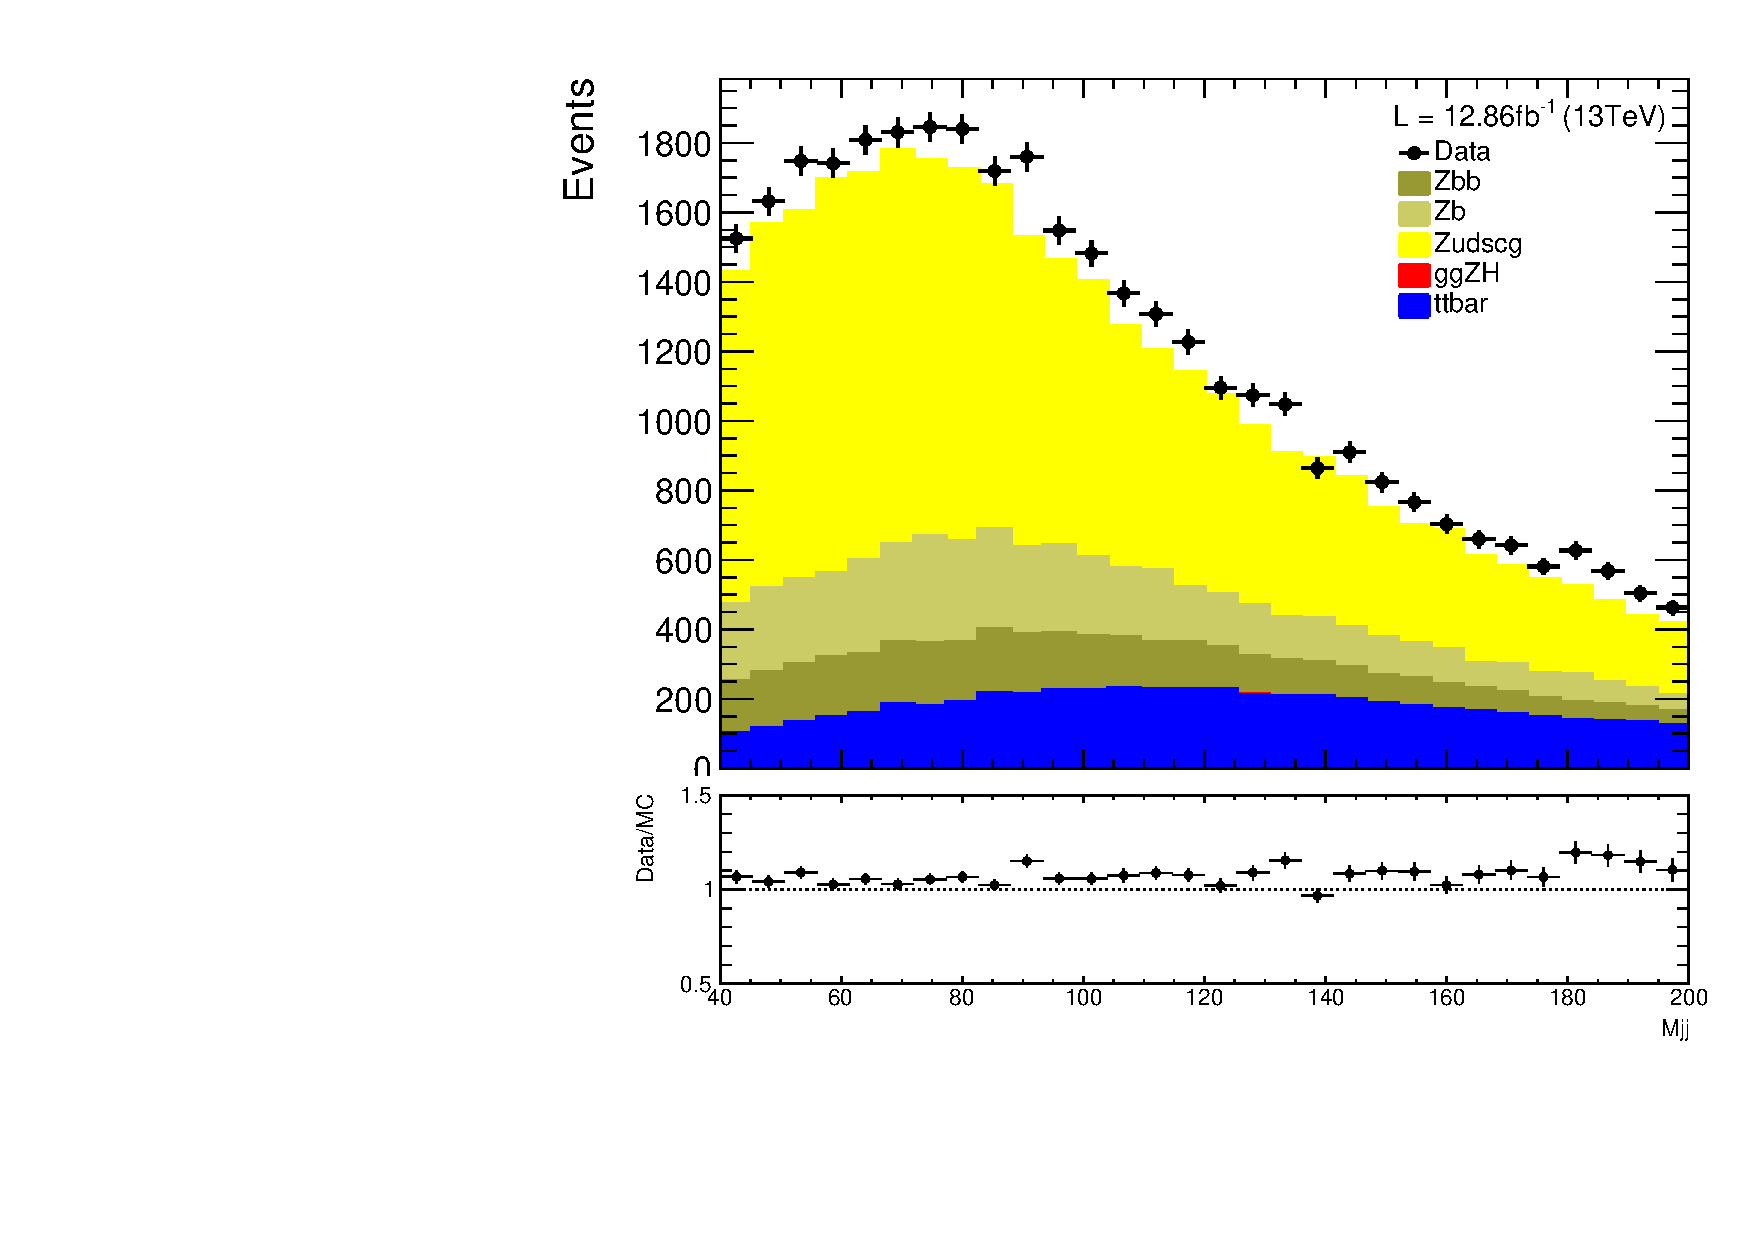
\includegraphics[width=0.32\textwidth]{b-reg/Vali_Data_MC_jet_16plus3_js_Mjj_all_Loose}\hfil
  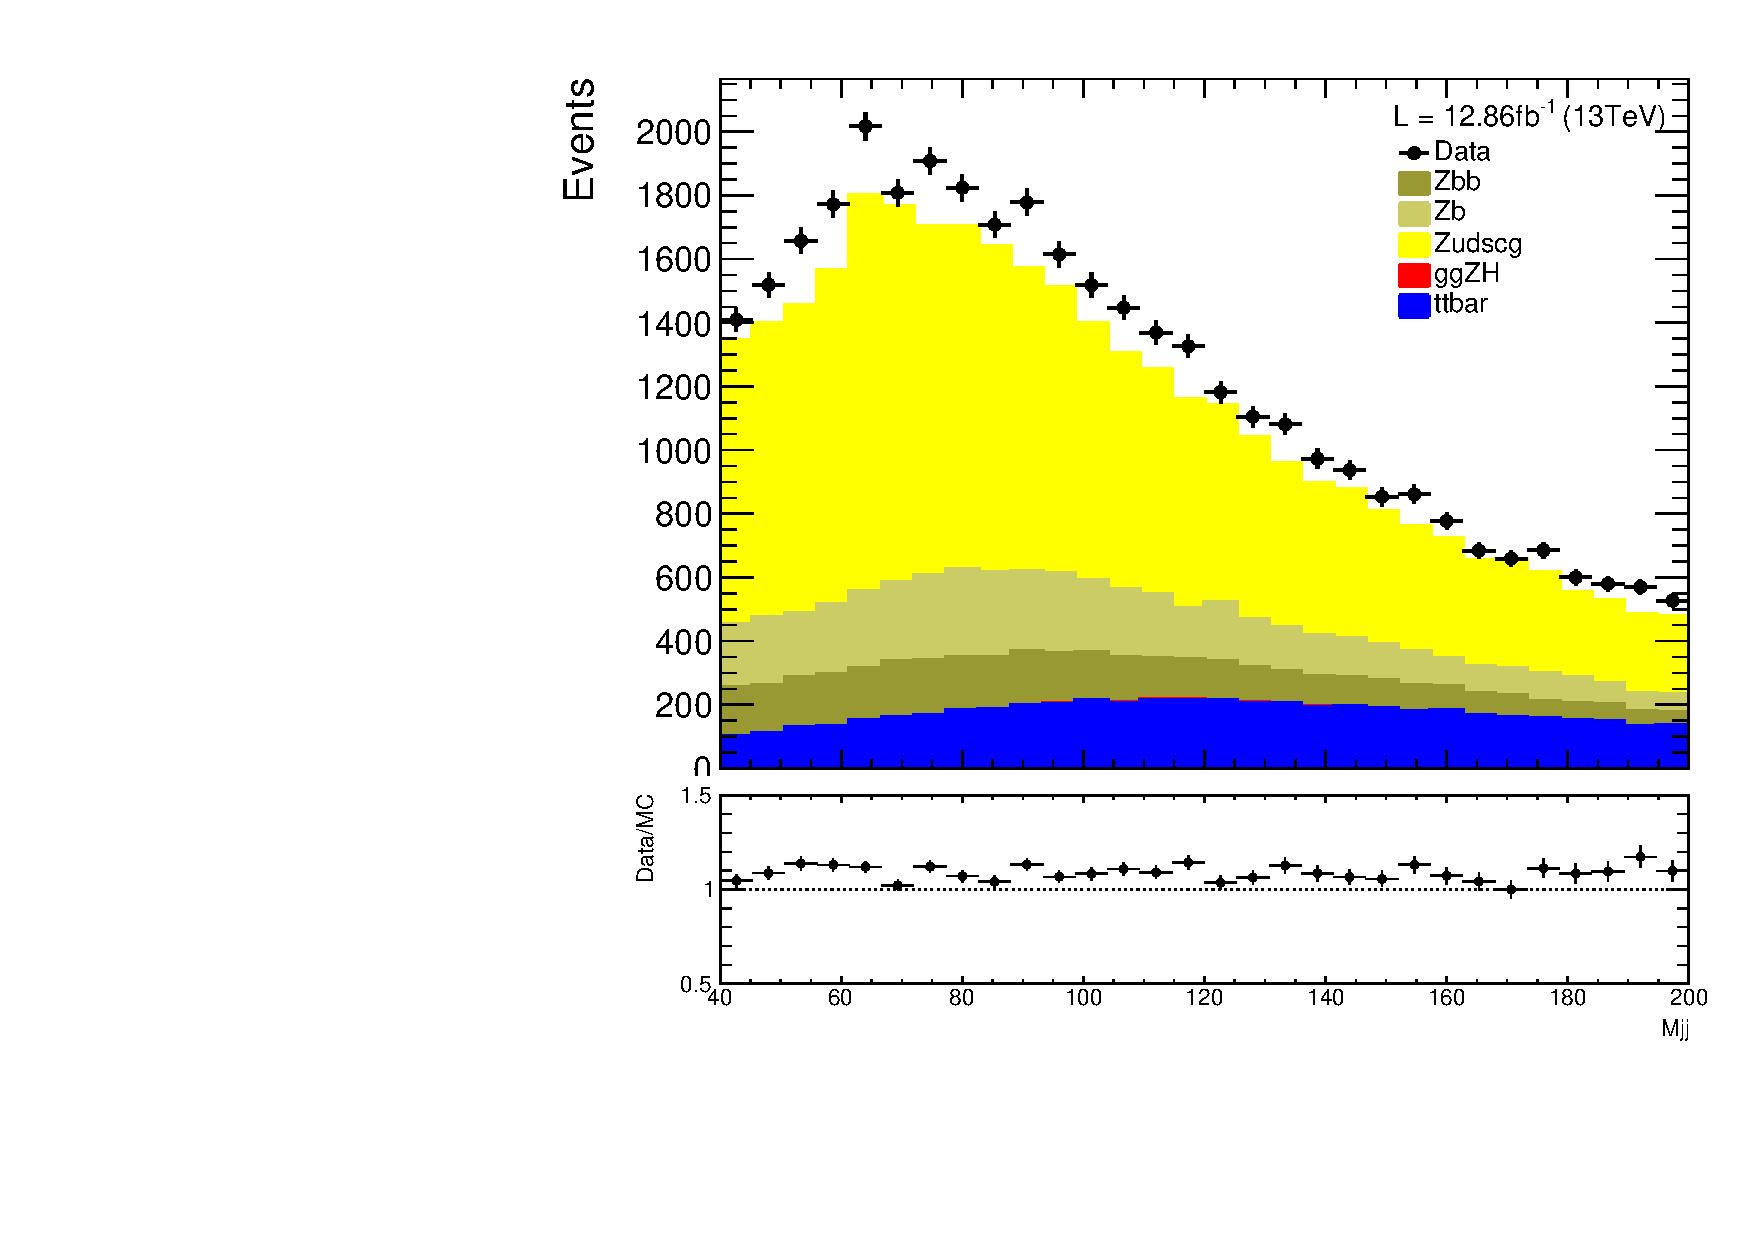
\includegraphics[width=0.32\textwidth]{b-reg/Vali_Data_MC_jet_Hbb_Mjj_all_Loose}\hfil\\
  \caption{Distributions of the $m_{jj}$. On the left
    are plots with no regression, in the center - using
    \textbf{16plus3 js} training and on the right - using \textbf{Hbb}
    regression.  Top plots for muon channel, middle for electron
    channel and bottom is the combination (sum) of the two.  }
  \label{fig:vali-Mjj}
\end{figure*}



%\clearpage
\subsection{Effect on the final results}
We are interested to know how much does the use of the jet energy
regression improves the final results -- the expected limit of the
analysis. Better $m_{jj}$ resolution allows for a tighter cut on that
variable which increases the significance of the signal. Or, in case of
2D($\Mgg, Mjj$) shape analysis it should also improve the limit.

We applied the above described regression (\textbf{16plus3 js}) and
Fig.~\ref{fig:b-reg-limits} shows the expected limit with and without
the use of regression.  The conclusion is: it works! and it brings
100500\% improvement in the limit!

\begin{figure*}[thb]
  \centering
  
\includegraphics[width=0.45\textwidth]{empty}\hfil
  
\includegraphics[width=0.45\textwidth]{empty}\hfil
  \caption{Expected limit without using b-jet energy regression (left)
    and with the regression (right).}
  \label{fig:b-reg-limits}
\end{figure*}


